%%%% DOCUMENT CLASS ************************************************************
%\documentclass[print,thumbmain]{src/thesis}  % uncomment for writing
\documentclass[final]{src/thesis} % uncomment for rendering/final version

%%%% PREAMBLE ******************************************************************
%!TEX root = ../thesis.tex
\usepackage{xcolor}

%% TU/e RED
\definecolor{thumbcolor}{RGB}{198,198,198}
\definecolor{deepcolor}{RGB}{0,0,0}
\definecolor{titlecolor}{RGB}{215,47,35}

%% DEEP PURPLE
% \definecolor{thumbcolor}{RGB}{200,200,200}
% \definecolor{deepcolor}{RGB}{70,25,200}
% \definecolor{titlecolor}{RGB}{120,80,235}

%% MATLAB BLUE
% \definecolor{thumbcolor}{RGB}{200,200,200}
% \definecolor{deepcolor}{RGB}{0,0,0}
% \definecolor{titlecolor}{RGB}{0,114,159}

%% PRUSA ORANGE
% \definecolor{thumbcolor}{RGB}{250,180,140}
% \definecolor{deepcolor}{RGB}{0,0,0}
% \definecolor{titlecolor}{RGB}{238,112,35}

%% SOFT ORANGE
% \definecolor{thumbcolor}{RGB}{250,180,140}
% \definecolor{deepcolor}{RGB}{0,0,0}
% \definecolor{titlecolor}{RGB}{250,180,140}

% \definecolor{C1}{RGB}{0,88,168}
% \definecolor{C2}{RGB}{202,30,4}
% \definecolor{C3}{RGB}{52,167,63}
% \definecolor{C4}{RGB}{238,112,35}

\definecolor{Matlab1}{RGB}{0,114,189}
\definecolor{Matlab2}{RGB}{217,83,25}
\definecolor{Matlab3}{RGB}{237,177,32}
\definecolor{Matlab4}{RGB}{126,47,142}
\definecolor{Matlab5}{RGB}{119,172,48}
\definecolor{Matlab6}{RGB}{77,190,238}
\definecolor{Matlab7}{RGB}{162,20,47}

\definecolor{C2}{RGB}{202,30,4}
\definecolor{C3}{RGB}{52,167,63}
\definecolor{C4}{RGB}{238,112,35}

\definecolor{magenta}{RGB}{255,20,120}
\definecolor{lightgreen}{RGB}{120,194,22}

\input{src/packages}
%!TEX root = ../thesis.tex

% Texts or
\renewcommand{\emph}[1]{'\textit{#1}'}
\newcommand{\sorotoki}{\textup{\texttt{SOROTOKI}} }
\newcommand{\matlab}{\textup{\texttt{MATLAB}} }
\newcommand{\data}[1]{(\raisebox{-2.7pt}{\textcolor{#1}{\,\Huge{\textbf{-}}}})}

% Equations/math
\newcommand{\be}{\begin{equation}}
\newcommand{\ee}{\end{equation}}
\newcommand{\benn}{\begin{equation*}}
\newcommand{\eenn}{\end{equation*}}
\newcommand{\bea}{\begin{eqnarray}}
\newcommand{\eea}{\end{eqnarray}}
\newcommand{\beann}{\begin{eqnarray*}}
\newcommand{\eeann}{\end{eqnarray*}}
\newcommand{\ba}{\begin{align}}
\newcommand{\ea}{\end{align}}
\newcommand{\bpm}{\begin{pmatrix}}
\newcommand{\epm}{\end{pmatrix}}
\newcommand{\bbm}{\begin{bmatrix}}
\newcommand{\ebm}{\end{bmatrix}}
\newcommand{\bc}{\begin{center}}
\newcommand{\ec}{\end{center}}
\newcommand{\pwr}[1]{\cdot10^{\textrm{#1}}}
\newcommand*{\myquotingsource}{}
\newenvironment{myquoting}[1]{%
  \renewcommand*{\myquotingsource}{#1}
  \begin{quoting}[font={itshape,raggedleft},leftmargin=0.5\linewidth,rightmargin=2em]%
}{%
  \par\medskip
  \myquotingsource
  \end{quoting}%
}

% Symbols and annotations
%\newcommand{\fB}{\boldsymbol{f}}
\newcommand{\maT}{\text{ma}}
\newcommand{\qR}{\mathrm{q}}
\newcommand{\RBB}{\mathbb{R}}
\newcommand{\rmsT}{\text{rms}}
\newcommand{\uB}{\boldsymbol{u}}
\newcommand{\xBF}{\mathbf{x}}
\newcommand{\interior}{\operatorname{int}}

% Tikz figures
\newcommand{\SF}{1}                 % Scaling factor
\newcommand{\TS}{\normalsize}       % Text size
\newcommand{\lw}{0.7pt}             % Line width
\newcommand{\TSTick}{\small}        % Text size axis labels
\newcommand{\axislabels}[2]{\foreach \x/\y/\s in {#1} {\node[#2,inner sep=1mm] at (\x,\y) {\TSTick $\s$};}}
\newcommand{\wheel}[3]{ \draw[line width=\lw] (#1,#2) circle (#3);
                        \fill[bottom color=MRblue!60!black!80,top color=MRblue!10] (#1,#2) circle (#3-0.5*\lw);
                        \fill[color=MRblue!30] (#1,#2) circle (#3-\lw);
                        \fill[top color=MRblue!60!black!80,bottom color=MRblue!10] (#1,#2) circle (0.7*#3);
                        \fill[color=MRblue!30] (#1,#2) circle (0.7*#3-\lw);
                        \fill[color=black] (#1,#2) circle (0.1*#3);}

\newcommand{\CoM}[3]{\filldraw[inner color=white,outer color=black!7!white,draw=black,line width=\lw] (#1,#2) circle (#3+0.5*\lw);
                     \begin{scope}[xshift=#1,yshift=#2]
                        \clip(-#3,0) -- (0,0) -- (0,#3) -- (#3,#3) -- (#3,0) -- (0,0) -- (0,-#3) -- (-#3,-#3) -- cycle;
                        \fill[inner color=black!50!white,outer color=black] (0,0) circle (#3);
                     \end{scope}}

\definecolor{MRdarkblue}{RGB}{16,9,88}      % Define a set of colors to be used throughout thesis
\definecolor{MRred}{RGB}{152,0,0}
\definecolor{MRgreen}{RGB}{0,146,69}
\definecolor{MRblue}{RGB}{53,153,204}
\definecolor{MRorange}{RGB}{220,85,30}
\definecolor{MRlightgreen}{RGB}{217,224,33}
\definecolor{MRyellow}{RGB}{255,214,0}
\definecolor{MRgrey}{gray}{0.95}
\usetikzlibrary{arrows}
\usetikzlibrary{patterns}
\usetikzlibrary{decorations.markings}
\usetikzlibrary{shadings}
\usetikzlibrary{shapes}

% Counters
\newcounter{ContNum}        % Counter for the contributions
\renewcommand{\theContNum}{\Roman{ContNum}}

% Other
\newcommand\blankfootnote[1]{%
  \let\thefootnote\relax\footnotetext{#1}%
  \let\thefootnote\svthefootnote%
}
\newcounter{numfootnote}
\newcommand\numfootnote[1]{%
    \stepcounter{numfootnote}%
    \newcommand{\thefootnote}{\thenumfootnote}%
    \footnote{#1}
}

\newcommand{\disclaimer}{\\[\baselineskip]  A detailed list of the differences between this chapter and the article on which it is based is provided in the %\hyperref[chap: Modifications]{\emph{Modifications}}
\emph{Modifications} chapter of this thesis.}
\newcommand{\itemheader}[1]{~\\ \noindent\textbf{#1.}\ \ }
\newcommand{\itemheaderNewpage}[1]{\newpage \noindent\textbf{#1.}\ \ }
\newcommand{\contribution}[2]{\refstepcounter{ContNum}#2 \vspace*{2.1mm}\begin{tcolorbox}[colback=black!2!white,colframe=black!20!white] \textbf{Contribution \Roman{ContNum}.} {\em #1} \end{tcolorbox}\vspace*{2.1mm}}
\newcommand{\objective}[1]{\begin{tcolorbox}[colback=black!2!white,colframe=black!20!white] {\em #1} \end{tcolorbox}}
\newcommand{\terminology}[2]{\begin{tcolorbox}[colback=black!2!white,colframe=black!20!white] {\textbf{Terminology: } \textbf{#1} \em #2} \end{tcolorbox}}
\newcommand{\cover}[1]{\ifprint{}\else\includepdf[pages=-]{#1}\cleardoublepage\fi}
\newcommand{\boxedtext}[2]{\vspace*{2.1mm}\begin{tcolorbox}[colback=black!2!white,colframe=black!20!white] {\em #1} \end{tcolorbox}\vspace*{2.1mm}}
\input{src/vector}
\input{src/mathematics}
\input{src/lemma}
\input{src/review}
\input{src/tikz}
\usepackage[version=3]{mhchem}
\usepackage{graphicx}
\usepackage{subfig}
\usepackage{amsmath}
\usepackage{soul}
\usepackage{CJKutf8}
\usepackage{quoting}
\DeclareMathOperator*{\argmin}{arg\,min}

%%%% Graphics paths
% **********************************************************
\graphicspath{{img/}{../../img/}{../../../img/}}
%%%% REVIEWING OF THESIS
% **********************************************************
%\usepackage{showframe}
\setreviewsoff

% see src/colors to change colors

%%%% DOCUMENT DETAILS **********************************************************
\author{Ralf Johannes Josephus Mackenbach}
\newcommand{\placeofbirth}{Eindhoven}
\renewcommand{\year}{2023}
\newcommand{\defensedate}{29 November 2023}
\newcommand{\defensetime}{13:30}
\newcommand{\maintitle}{Available Energy}
\newcommand{\subtitle}{A compass for navigating the nonlinear landscape of fusion plasma turbulence}
\newcommand{\isbn}{TO-BE-ADDED}     % 123boldmath-45-678-9012-3
\newcommand{\rector}{prof. dr. Silvia Lenaerts}
% other relevant meta data about the thesis can be found in preface.tex

\makeatletter % generates all the \author stuff
%%%% MAIN DOCUMENT *************************************************************

\begin{document} 
%%%%%%%%%%%%%%%%%%%%%%%%%%%%%%%%%%%%%%%%%%%%%%%%%%%%%%%%%%%%%%%
%%%% ***************************************************************************
\pagenumbering{roman}
\thispagestyle{empty}

%%%% FRONT MATTERS *************************************************************
\cover{thesis_front.pdf}    % Adds your thesis' front cover if the option 'print' is NOT used. Printing companies require the thesis cover to be supplied separately and in a different format. Definition of \cover{} is given in commands.tex.

% Front matter
%!TEX root = ../thesis.tex
% First page
\thispagestyle{empty}
\vspace*{30mm}\noindent
\begin{center}
{\LARGE\maintitle}\\[7mm]
{\Large\subtitle}\\[4.5cm] %\\[7mm]
{\Large \@author}
\end{center}

\newpage
\thispagestyle{empty}

% Page with c logo etc.
\vspace*{\fill}

\hspace*{-7mm}\includegraphics[width=6cm]{TUeLOG_new.eps}\\
{\small The work described in this thesis was carried out at the Eindhoven University of
Technology.}\\[8mm]


\noindent\bgroup\small
A catalogue record is available from the Eindhoven University of Technology Library.\\
ISBN: \isbn\\[4mm]
Typeset by the author using the pdf \LaTeX \ documentation system.\\
Cover design: Igor Hoogerwoord Tan \\
\textsuperscript{\copyright}\year \; by \@author. All rights reserved.
\egroup

\newpage
\thispagestyle{empty}


% Title page

\vspace*{30mm}
\begin{center}
{\LARGE\maintitle}\\[7mm]
{\Large\subtitle}\\[30mm] %\\[7mm]
{\large\textsc{Proefschrift}}\\[8mm]
ter verkrijging van de graad van doctor aan de\\
Technische Universiteit Eindhoven, op gezag van de\\
rector magnificus \rector, voor een\\
commissie aangewezen door het College voor\\
Promoties, in het openbaar te verdedigen\\
op \defensedate\ om \defensetime\ uur\\[8mm]
door\\[8mm]
\@author\\[8mm]
geboren te \placeofbirth
\end{center}
\vfill

\newpage
\thispagestyle{empty}

\noindent
Dit proefschrift is goedgekeurd door de promotoren en de samenstelling van de promotiecommissie is als volgt:\\[7mm]

\noindent
\begin{tabular}{@{}l p{9.8cm}}
% voorzitter:                 &   prof. dr. N.J. Lopes Cardozo \\                \\
promotor:                   &   prof. dr. N.J. Lopes Cardozo \\
promotor                    &   prof. dr. P. Helander \\
co-promotor:                &   dr. J.H.E. Proll \\
leden:                      &   prof. dr. M. Barnes \\
                            &   dr. ir. J. Van Dijk \\
                            &   dr. P. Ricci \\
                            &   dr. E.J. Paul \\
\end{tabular}

\vfill
\noindent
Het onderzoek dat in dit proefschrift wordt beschreven is uitgevoerd in overeenstemming met de TU/e Gedragscode Wetenschapsbeoefening.

\chapter*{Foreword}
I won't spoil all the nice things I'll say here yet, stay tuned for the final version :-)
%*********************************************************************************%
\chapter*{Summary} % Try to keep within approx 350 words / one page
\addcontentsline{toc}{chapter}{Summary}
\markboth{Summary}{Summary}


\begin{center}
\rule{\textwidth}{.75pt}\vspace*{1mm}
\textbf{{\Large Available Energy\\[2mm] \textit{A compass for navigating the nonlinear landscape of fusion plasma turbulence}}}
\rule{\textwidth}{.75pt}
\end{center}
\vspace*{2ex}
Nuclear fusion, the process in which light atomic nuclei combine to form heavier nuclei, releases large amounts of energy, with its specific energy (the energy per unit mass of fuel) being roughly a factor $\sim 10^7$ larger than that of gasoline. Furthermore, this process (which powers many of the stars in our universe) does not emit greenhouse gases, and both these qualities make it an attractive energy source. Magnetic confinement fusion attempts to realise this goal by confining the hot fuel, an ionised plasma at roughly 150 million degrees centigrade, with a strong magnetic field of several Tesla. Importantly, this fuel needs to be well insulated so that one can maintain the high temperature required. However, the plasma exhibits turbulence, which degrades the insulation and makes it more difficult to achieve the desired properties. \par
In this thesis, we investigate the merit of a thermodynamic quantity, called available energy (\AE{}), as a measure of turbulence in fusion plasmas. Importantly, a deeper understanding of such turbulence can aid in attaining much-improved fusion reactor performance, hopefully bringing magnetic confinement fusion closer to a reality. Available energy derives its name from the fact that it is an upper bound on the amount of thermal energy that may be extracted from the plasma, subject to a number of constraints, i.e. it is the amount of energy which is {\it available} to be liberated. Although this quantity first appeared in the realm of mathematics nearly a century ago, it has found fairly little use as a turbulence measure. In this thesis, we make a first attempt at such an investigation by specialising to the so-called trapped electrons, which are trapped in a region of weaker magnetic field strength. The regions where such particles are trapped are decided by the magnetic field $\boldsymbol{B}$, and the functional form of this field is often called its geometry. \par 
To calculate the \AE{}, we first develop methods and benchmarks for accurately calculating emblematic quantities of such trapped particles, as they will enter the calculation of \AE{}. With these numerical routines in place, the \AE{} of trapped electrons in general geometries is analytically derived in the limit of a flux tube, a slender domain around a magnetic field line that is everywhere parallel to the magnetic field. This expression for \AE{} is then calculated for a number of geometries for which nonlinear turbulence simulations exist and compared against the results of these simulations. Comparing the turbulent energy flux (i.e., the amount of energy per unit time per unit area that passes through the domain in the fully turbulent state) with \AE{}, we find that the two are correlated via a power law, highlighting that \AE{} points to fundamental properties of the turbulence. To further investigate the various dependencies \AE{} exhibits, we go on to specialise in tokamaks. This allows one to readily investigate how \AE{} changes as one varies the magnetic shear, the pressure gradient, the triangularity, and other figures of merit central in tokamaks. This reproduces some known trends, such as the highly beneficial nature of negative magnetic shear, and allows us to make qualitative statements on the benefits of negative triangularity. \par 
All in all, we find that \AE{} is a useful measure of turbulence, opening up computationally cheap methods to estimate turbulence levels without the need for nonlinear simulations. It also provides insight into why some configurations are favourable to others, due to the fact that \AE{} is easy to interpret. Looking further into the future, possible generalisations could extend the domain of utility of \AE{} beyond trapped electrons, making it a useful tool in more general scenarios. If such a generalisation proves successful, finding geometries in which turbulence is much reduced may then be achieved, ultimately bringing fusion power closer to reality.

\vspace*{11pt}\noindent
\textbf{Keywords:} \ \ Plasma turbulence, Fusion plasma, Available energy, Plasma thermodynamics, Magnetic confinement fusion, Gyrokinetics
%*********************************************************************************%
\chapter*{Samenvatting}
\addcontentsline{toc}{chapter}{Samenvatting}
\markboth{Samenvatting}{Samenvatting}

Kernfusie, het proces waarbij lichte atoomkernen samenkomen om zwaardere kernen te vormen, geeft grote hoeveelheden energie vrij, waarbij de specifieke energie (de energie per eenheid massa brandstof) ongeveer een factor $\sim 10^7$ groter is dan die van benzine. Bovendien stoot dit proces (dat veel van de sterren in ons heelal aandrijft) geen broeikasgassen uit, en deze eigenschappen maken het tot een aantrekkelijke energiebron. Magnetische opsluitingsfusie probeert dit doel te bereiken door de hete brandstof, een geïoniseerd plasma bij ongeveer 150 miljoen graden Celsius, te omringen met een sterke magnetische veldsterkte van enkele Tesla. Belangrijk is dat deze brandstof goed geïsoleerd moet zijn om de hoge vereiste temperatuur te behouden. Echter, het plasma vertoont turbulentie, wat de isolatie verslechtert en het moeilijker maakt om de gewenste eigenschappen te bereiken. \par
In deze scriptie onderzoeken we de waarde van een thermodynamische grootheid, genaamd beschikbare energie (\AE{}), als een maat voor turbulentie in fusieplasma's. Belangrijk is dat een dieper inzicht in dergelijke turbulentie kan helpen bij het verbeteren van de prestaties van fusiereactoren, hopelijk dichter bij de realiteit van magnetische opsluitingsfusie brengend. Beschikbare energie dankt zijn naam aan het feit dat het een bovengrens is voor de hoeveelheid thermische energie die uit het plasma kan worden onttrokken, onderhevig aan een aantal beperkingen, d.w.z. het is de hoeveelheid energie die {\it beschikbaar} is om te worden vrijgegeven. Hoewel deze grootheid bijna een eeuw geleden voor het eerst verscheen in de wiskunde, heeft het als maat voor turbulentie relatief weinig toepassing gevonden. In deze scriptie doen we een eerste poging tot een dergelijk onderzoek door ons te specialiseren in zogenaamde gevangen elektronen, die gevangen zitten in een gebied met een zwakkere magnetische veldsterkte. De gebieden waarin deze deeltjes gevangen zitten, worden bepaald door het magnetische veld $\boldsymbol{B}$, en de functionele vorm van dit veld wordt vaak de geometrie ervan genoemd. \par
Om de \AE{} te berekenen, ontwikkelen we eerst methoden en referentiewaarden om nauwkeurig hoeveelheden te berekenen die kenmerkend zijn voor dergelijke gevangen deeltjes, aangezien deze de berekening van de \AE{} zullen binnengaan. Met deze numerieke routines wordt de \AE{} van gevangen elektronen in algemene geometrieën analytisch afgeleid in de limiet van een fluxbuis, een smal domein rond een magnetische veldlijn die overal evenwijdig loopt aan het magnetische veld. Deze uitdrukking voor de \AE{} wordt vervolgens berekend voor een aantal geometrieën waarvoor niet-lineaire turbulentiesimulaties bestaan, en vergeleken met de resultaten van deze simulaties. Door de turbulente energiestroom (dat wil zeggen de hoeveelheid energie per eenheid tijd per eenheid oppervlakte die door het domein stroomt in de volledig turbulente toestand) te vergelijken met de \AE{}, ontdekken we dat de twee gecorreleerd zijn via een machtsverband, wat aangeeft dat \AE{} wijst op fundamentele eigenschappen van de turbulentie. Om de verschillende afhankelijkheden die \AE{} vertoont verder te onderzoeken, gaan we over op het specialiseren van tokamaks. Dit stelt ons in staat om gemakkelijk te onderzoeken hoe \AE{} verandert wanneer men de magnetische schuif, het drukgradient, de driehoekigheid en andere kenmerken die centraal staan in tokamaks, varieert. Dit reproduceert enkele bekende trends, zoals de zeer gunstige aard van negatieve magnetische schuif, en het stelt ons in staat om kwalitatieve uitspraken te doen over de voordelen van negatieve driehoekigheid. \par
Al met al vinden we dat er waarde zit in \AE{} als een maat voor turbulentie, waardoor er goedkope rekenmethoden ontstaan om turbulenieniveaus te schatten zonder de noodzaak van niet-lineaire simulaties. Het biedt ook inzicht in waarom sommige configuraties gunstiger zijn dan andere, omdat \AE{} gemakkelijk te interpreteren is. Kijkend naar de toekomst toe, zouden mogelijke generalisaties het nut van \AE{} voorbij gevangen elektronen kunnen uitbreiden, waardoor het een nuttig hulpmiddel wordt in meer algemene scenario's. Als zo'n generalisatie succesvol blijkt te zijn, kan het gemakkelijk geometrieën vinden waarin turbulentie sterk verminderd is, wat uiteindelijk fusie-energie dichter bij de realiteit kan brengen.


\vspace*{11pt}\noindent



%*********************************************************************************%
\chapter*{Societal summary}
\addcontentsline{toc}{chapter}{Societal summary}
\markboth{Societal summary}{Societal summary}

In the core of stars light atomic nuclei combine to form larger nuclei, a process called nuclear fusion, releasing large amounts of energy. If one were able to harness all the energy, 1 milligramme of fusion fuel (e.g. hydrogen) would release roughly the same amount of energy as 10 kilogrammes of gasoline. Besides this high efficiency of the fusion fuel, it furthermore does not release greenhouse gases as it burns, making it an attractive energy source. However, the conditions required for nuclear fusion to occur are quite extreme, with the fuel temperature close to 150 million degrees centigrade. At such temperatures, the fuel is a fully ionised plasma in which electrons are detached from their atomic nuclei. This plasma is not unlike a ``charged fluid '', and it responds to electromagnetic fields. \par  
One needs a way of confining the plasma, so that the hot plasma does not come into contact with a cool material wall. Since the plasma responds to magnetic fields, one can use the magnetic force to confine the plasma, and this method of attaining nuclear fusion is called magnetic confinement fusion. Note that in order to generate the magnetic field one requires large superconducting coils which need to be cooled to a few degrees Kelvin. We thus have a plasma of some 150 million degrees centigrade, confined with superconducting coils which are close to zero Kelvin, and these are within metres of each other. This large gradient can be sustained only if the plasma sufficiently insulating. However, these large gradients also give rise to turbulence. \par
This turbulence is similar to pouring milk into a cup of tea; the differences in velocity, density, and temperature between milk and tea give rise to all kinds of swirls and whirls, ultimately mixing the milk and the tea into a homogeneous whole. So, too, does the turbulence in the fusion reactor mix the hot and cold regions, which makes it more difficult to sustain the desired 150 million degrees centigrade. Understandably, much research has been devoted to understanding how turbulence arises in these reactors, so that we may control and suppress it. \par 
In this thesis, we tackle this problem by taking a step back from all the complex details of the turbulence and instead looking at budgets of energy. That is, we ask ourselves the question how much energy can at most reside in the all swirls of the turbulence, without actually considering what the whirly patterns may look like. This enables one to find easy-to-calculate expressions, and we subsequently compare this calculation of the energy-budget with actual turbulence as computed by a supercomputer. We find that there is correspondence between the two, showcasing that there is some structure in the turbulent chaos. This makes it possible to, computationally speaking, cheaply estimate the levels of turbulence in a fusion reactor, which could aid in designing better reactors in the long run. 

%%%% NOMENCLATURE **************************************************************
\cleardoublepage
\pdfbookmark{\contentsname}{Contents}
\tableofcontents

\newpage
\newenvironment{Nomen}
    {\vspace*{-3mm}\begin{center}
    \begin{longtable}{p{.15\textwidth} p{.83\textwidth}}
    }
    {
    \end{longtable}
    \end{center}\vspace*{-1.2cm}
    }
\newcommand{\AddSymbol}[2]{#1 & #2 \\}




%*********************************************************************************%
\chapter*{Nomenclature}
\addcontentsline{toc}{chapter}{Nomenclature}
\markboth{Nomenclature}{Nomenclature}








%*********************************************************************************%



\section*{Acronyms}

\begin{Nomen}
\AddSymbol{\AE{}}{Available Energy}
\AddSymbol{TEM}{Trapped electron mode}
\AddSymbol{ITG}{Ion temperature gradient mode}
\AddSymbol{ETG}{Electron temperature gradient mode}
\AddSymbol{UI}{Universal instability}
\AddSymbol{BAD}{Bounce-averaged drift}
\AddSymbol{QS}{Quasi-symmetric}
\AddSymbol{QI}{Quasi-isodynamic}
\end{Nomen}


%*********************************************************************************%
%\newpage
\section*{Operators and  symbols}

\begin{Nomen}
\AddSymbol{$\left(\frac{\partial f}{\partial x}\right)_{\boldsymbol{y}}$}{Partial of $f$ with respect to $x$, at constant $\boldsymbol{y}$. Also denoted as $(\partial_x f)_{\boldsymbol{y}}$}
\AddSymbol{$x \in \mathcal{X}$}{Element $x$ is a member of the set $\boldsymbol{X}$}
\AddSymbol{$\mathcal{Y} \subseteq \mathcal{X}$}{The set $\mathcal{Y}$ is a subset of the set $\mathcal{X}$}
\AddSymbol{$\dot{x}$}{Temporal derivative of $x(t)$, i.e. $\dot{x} \equiv \partial_t x$}
\AddSymbol{$\boldsymbol{B}$}{The magnetic field}
\AddSymbol{$\boldsymbol{A}$}{The magnetic potential which satisfies $\nabla \times \boldsymbol{A} = \boldsymbol{B}$}
\AddSymbol{$B$}{The magnetic field strength, i.e. $B \equiv |\boldsymbol{B}|$}
\AddSymbol{$\boldsymbol{v}$}{The particle velocity}
\end{Nomen}

%*********************************************************************************%
\section*{Often used terms}

\begin{Nomen}
\AddSymbol{Gyroradius}{The radius of the circular motion of a charged particle in a magnetic field}
\AddSymbol{Omnigeneity}{A property of a magnetic field, in which trapped particles are radially stationary}
\end{Nomen}

%\thispagestyle{empty}


%%%% MAIN MATTERS *************************************************************
% This state variable is used for creating the thumb index by indicating that
% the following chapter is numbered (i.e. not \chapter*{})
\isstarredchapterfalse
\cleardoublepage
\thispagestyle{empty}
\setcounter{page}{1}
\pagenumbering{arabic}
\part{Background}\label{part: background}
\chapter{Introduction}
\label{chap: intro}
%\thispagestyle{empty}
\setcounter{page}{1}
\pagenumbering{arabic}


As humanity has continued on its journey into the future, there has been steady increase in the amount of energy used by humanity on the whole, and per capita. With this increased energy usage came a plethora of ``luxuries'' ranging from cars to computers. Many of these machines have become so essential to daily living that we forget that most of our ancestors had to live without them. Indeed, this perceived correlation between how technologically advanced a civilisation is and the amount of power it produces can be used to construct a ranking system called the ``Kardashev'' scale, where the total power produced is used as the figure of merit \cite{gray2020extended}. Taking this number to be a crude measure of the maturity of a civilisation and assuming that our civilisation wishes to become more mature, it should be clear that we should search for new energy sources enabling us to climb the ranks. More specifically, sources of energy which deplete should be phased out as we look for renewable alternatives in our quest for growth. There are only a few sources which fit the bill and are within arm's length. Nuclear fusion, the process by which lighter nuclei combine to form heavier ones, is one of these few sources, and it is also the only energy source within reach that we know exists but have not been able to harness.\footnote{One may object to this statement, by noting that there exist processes which harness energy from black holes \cite{opatrny2012black,tursunov2019fifty,comisso2021magnetic}. However, seeing that such processes shall not be realised in the foreseeable future, we ignore them here.} \par 

A second reason to investigate fusion is the more acute problem of anthropogenic climate change. The burning of fossil fuels has subjected the atmosphere of the Earth to a dramatic increase in the amount of carbon dioxide, and this carbon dioxide acts as a greenhouse gas, retaining more of the heat of the earth. The greenhouse effect, combined with many climate feedback mechanisms \cite{schneider1972cloudiness,hansen1984climate,curry1995sea,dean2018methane}, can lead to a significant increase in average temperatures and sea levels. A rise in sea levels is evidently problematic for population hubs which are close to sea, one of which being the Netherlands in which the current thesis is to be defended. Thus, a reduction in our emissions of these greenhouse gases is required, and we must turn to renewable energy sources to do so. Along with e.g. wind, solar, and fission, nuclear fusion is such a renewable energy source, and if it becomes a viable energy source in the near-future, it can aid in the energy transition. \par 

\vspace*{-2mm}
\section{A crash course in nuclear fusion}
\label{sec: chap1 motivation}

So, if nuclear fusion as an energy source is desirable, why is it not here yet? The main difficulty lies in the extreme conditions required to allow nuclear fusion to occur. This process involves fusing light atomic nuclei, with which a large amount of energy is released. In order to allow atoms to fuse one needs to overcome the Coulomb barrier, the mutual repulsion of positively charged atomic nuclei, and when the atomic nuclei are within close enough proximity the strong nuclear force binds them together. To get a feeling for the type of conditions needed to overcome this barrier, it is useful to look at a natural fusion reactor: the sun. In the fusing core of the sun, the mass density is approximately 10 times that of lead and the temperature is about 15 million degrees \textcelsius. Such conditions are indeed extreme, especially if one is to extract more energy from the fuel than is required to run it. We may somewhat relax the conditions required by choosing a fusion reaction with one of the largest cross sections. \par 

On earth, then, we focus on the fusion of the deuterium and tritium isotopes of hydrogen. These fuse together to become helium and a neutron, with $17.6$ MeV of kinetic energy, i.e.
\begin{equation*}
    \ce{^{2}_{1} D} + \ce{^{3}_{1} T} \rightarrow \ce{^{4}_{2} He} + \ce{^{1}_{0} n} + 17.6 \: \mathrm{MeV}. 
\end{equation*}
To allow this fusion process to occur efficiently, the fuel must be heated to some 150 million degrees \textcelsius, and the fuel is a plasma. This hot plasma cannot be confined by means of a simple container: if the cool container wall came into contact with the hot plasma, the plasma would quickly cool. This problem may be circumvented in two manners; one can confine the fuel using its inertia (i.e. heating up the fuel in a short enough time-scale that its inertia keeps the fuel contained), or one can confine the ionised plasma by means of magnetic fields. The current thesis focusses on the latter. \par 

The topology of the confining magnetic field is required to be of a very particular form, ultimately a consequence of the Poincar\'e-Hopf theorem \cite{hopf1927vektorfelder}, though it may be understood in simpler terms.\footnote{We shan't focus on them here but there exist fusion concepts which have differing magnetic topologies, e.g. so-called linear devices as used in gas-dynamic multiple-mirror traps \cite{burdakov2011concept,beklemishev2013novosibirsk,ivanov2017gas}, or more recent designs proposed by start-ups such as Helion \cite{waldrop2014fusion}. Although a healthy amount of scepticism is recommended for these less orthodox approaches to nuclear fusion, it would be folly to categorically disregard them.} To the lowest order in the smallness of the gyroradius, charged particles stick to magnetic field lines like beads on a string. To avoid the ``beads'' being lost at the ends of the magnetic field line, one can require that the magnetic field line is in the shape of a circle so that ends do not exist. Such a {\it toroidal field component} can be achieved by bending a cylindrical solenoid into the shape of a torus. \par 
\begin{figure}
    \centering
    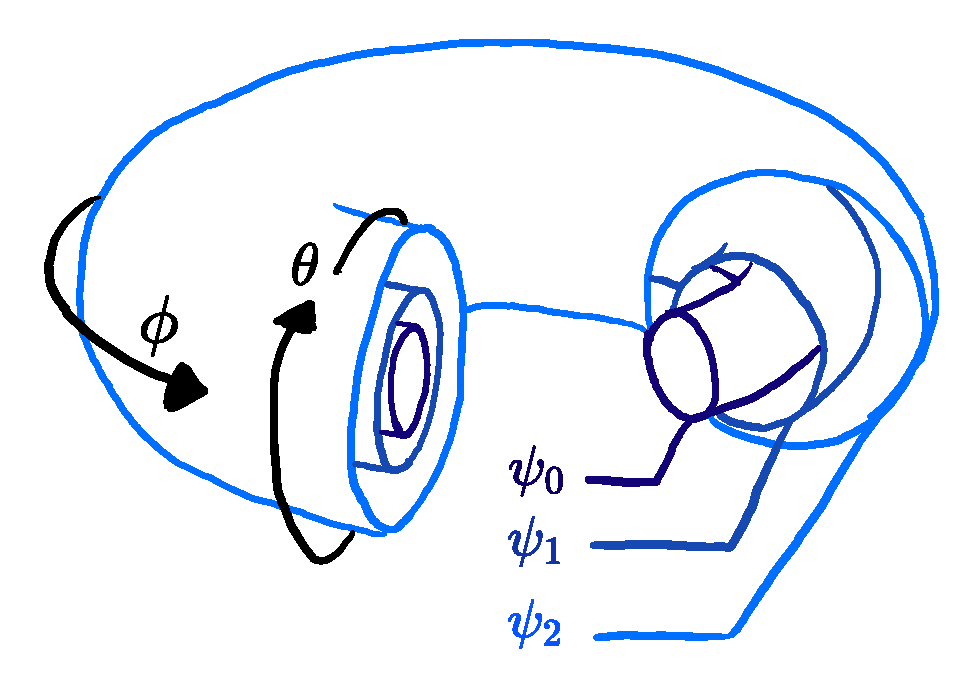
\includegraphics[width=0.6\textwidth]{3_chapters/0_introduction/img/tokamak.pdf}
    \caption{A schematic of a toroidal device. Here $\psi$ labels the various flux-surfaces, $\theta$ parameterises the poloidal angle, and $\phi$ parameterises the toroidal angle.}
    \label{fig: torus schematic}
\end{figure}
However, due to the finite gyroradius of the particles, they drift away from the field line (see \citet{blank2004guiding} for expressions of this drift), and the particles ultimately end up on the reactor wall. This may be remedied by introducing a {\it poloidal field component,}, as shown explicitly in \citet{helander2014theory}, ensuring that particles stay on the magnetic field lines. In total, we thus require that the magnetic field lines go both the long (toroidally) and short way (poloidally) around the torus, and the magnetic field lines live on tori.\footnote{To be more precise, the magnetic field lines may have three distinct topologies. Firstly, the magnetic field line may loop back on itself on the torus surface, resulting in a torus knot \cite{livingston1993knot,smiet2017knots}, and such surfaces are called rational. Second, it may never loop back on itself and trace the entire surface, and such surfaces are called irrational. Lastly, the magnetic field line may fill a volume chaotically, and the magnetic field is said to be chaotic in such situations. The last of these topologies is undesirable, and we ignore such fields here.} This allows the magnetic field line, and with it the plasma, to sample the surface and equilibrate on it. The transport problem is now reduced to one spatial dimension; we wish to find typical equilibrium quantities (e.g. density and temperature) as a function of the torus surface. A schematic of the geometry and typical coordinates that describe the torus is given in Fig. \ref{fig: torus schematic}.
\par 
In total we have thus found that magnetic field lines live on surfaces of tori (referred to as flux surfaces), winding both the short and long way around the torus. Each surface may then be characterised by the amount of ``twist'' of magnetic field lines on it, which is often denoted as $\iota$, the rotational transform. Quantitatively, it can be measured by following a magnetic field line of length $L$ around the torus and keeping track of the number of poloidal and toroidal turns. The rotational transform is then defined as the limit
\begin{equation}
    \iota = \lim_{L \rightarrow \infty} \frac{\textnormal{\# poloidal turns}}{\textnormal{\# toroidal turns}}.
    \label{eq: rotational transform integer definition}
\end{equation}
As stated before, inducing a toroidal component of the magnetic field can readily be achieved by bending a cylindrical solenoid into the shape of a torus. Attaining a poloidal component is less straightforward, and here we find a fork in the road that separates fusion power plant concepts.

\subsubsection*{The tokamak}
If we assume that our toroidal field is axisymmetric, that is, the torus is invariant under toroidal rotation, there is only one way to generate the poloidal component. As one can understand from Amp\`ere's circuital law, a toroidal current provides the required poloidal component. Indeed, the \textit{tokamak} employs this method to achieve confinement and is currently the most technologically mature concept of fusion power plants. A schematic showing its essential components is provided in Fig. \ref{fig: tokamak schematic}.
\begin{figure}
    \centering
    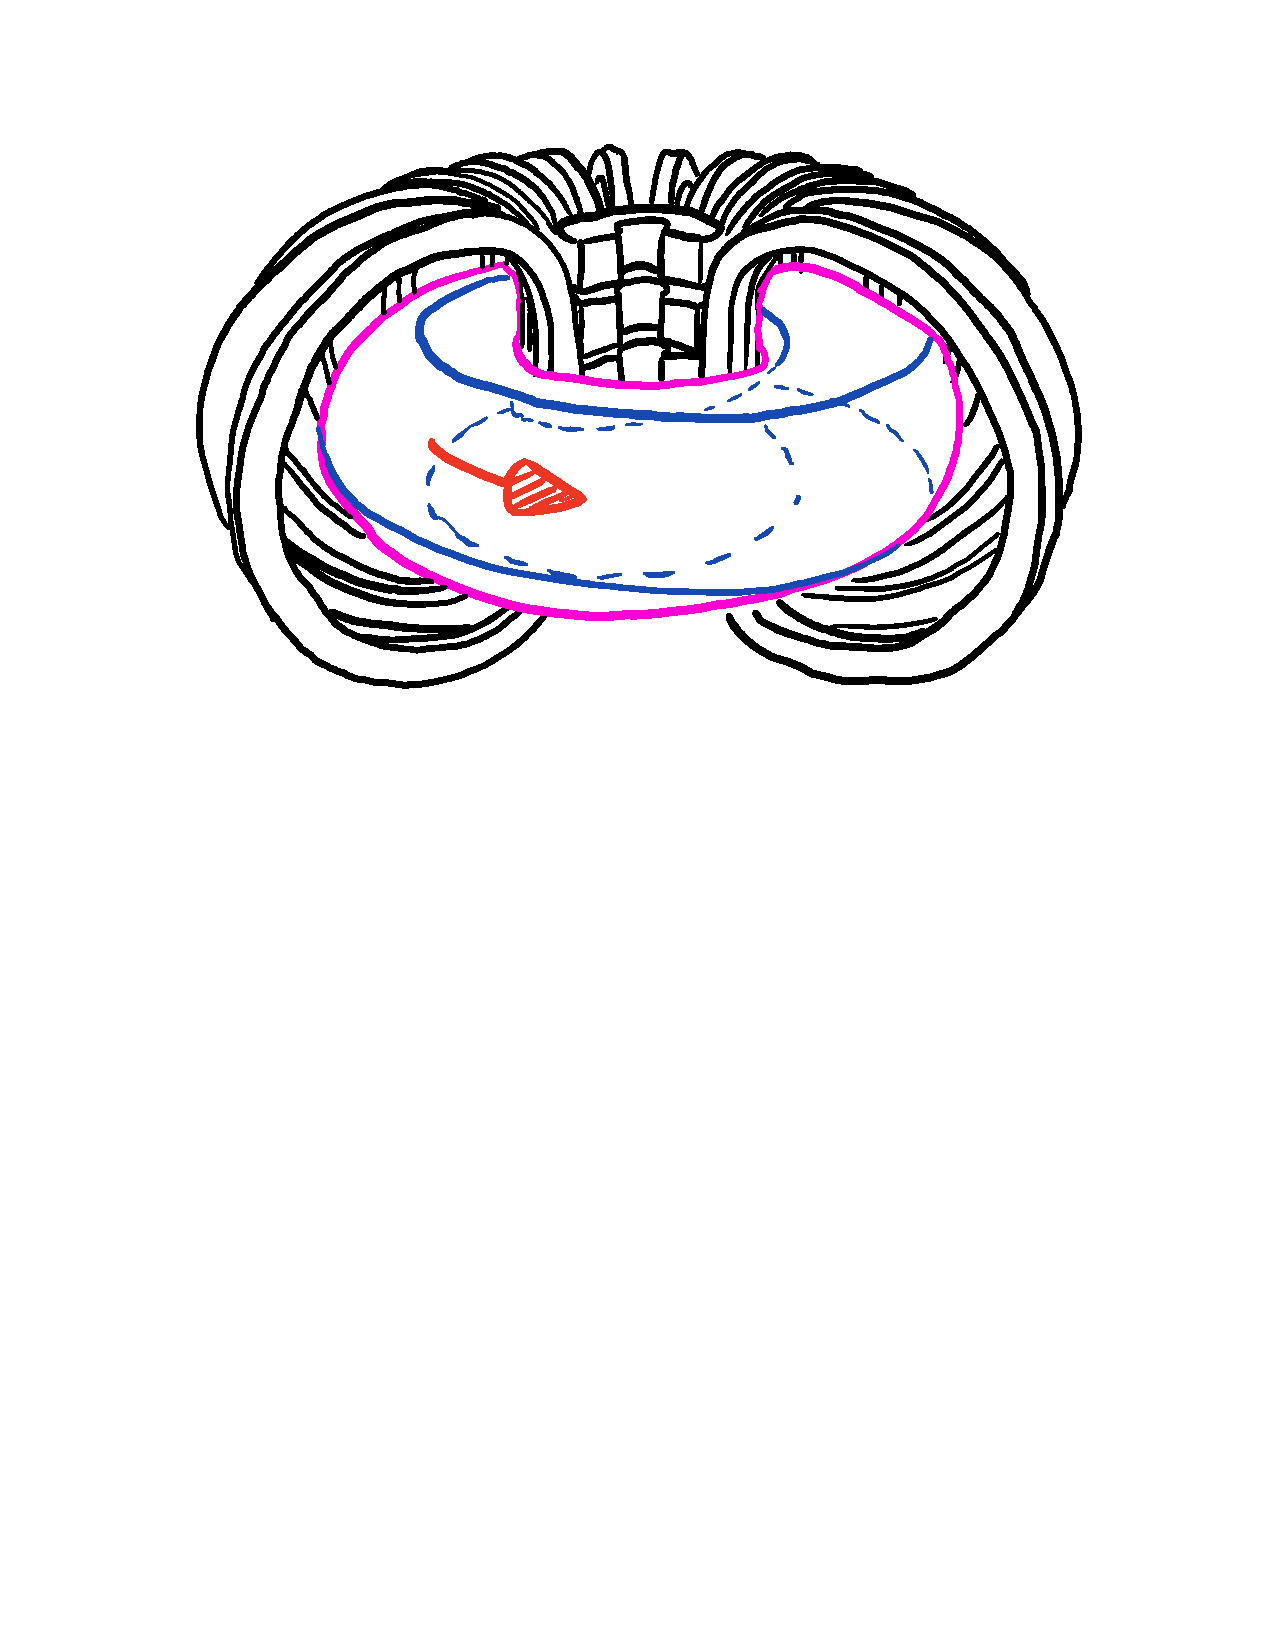
\includegraphics[width=0.5\textwidth]{3_chapters/0_introduction/img/tokamak-sketch.pdf}
    \caption{A schematic of the tokamak. In purple we see the outline of a flux-surface, in blue a field line which is situated on the flux-surface, in black we see the coils providing the necessary magnetic field, and in red we see an arrow representing the plasma current.}
    \label{fig: tokamak schematic}
\end{figure}
\par 
After its inception in 1950 in the U.S.S.R. by Andrei D. Sakharov and Igor E. Tamm, the tokamak made large strides in the late 1960s with the T-3A experiment reaching temperatures 10 times that of any other fusion power plant concept \cite{azizov2012tokamaks}. This solidified the tokamak's position as the leading concept, and we still feel the reverberations. Although the tokamak does have a number of advantages, it also suffers from problems that must be taken seriously. For example, in tokamaks a violent instability can arise, called a disruption, and in full-scale reactors it may irreparably break the device. The source of this Achilles' heel is the large current required to generate the poloidal magnetic field, and many are considering current-free alternatives to the tokamak.

\subsubsection{The stellarator}
The \textit{stellarator} provides this current-free path to confinement and has a more stable equilibrium without interruptions. The requirement of a current-free device necessitates that the torus is three-dimensional, in order to have rotational transform. As shown by \citet{mercier1964equilibrium}, one can generate a rotational transform by having current, ellipsoidally shaped cross sections which rotate as one travels toroidally around the torus, and by having torsion of the magnetic axis. The first solution is the one employed by the tokamak, and the latter two nonaxisymmetric solutions by the stellarator, and a sketch of the stellarator may be found in Fig. \ref{fig: sketch stellarator}. \par

The stellarator was first proposed in 1951 by Lyman Spitzer Jr. (head of the Princeton Astrophysics Department in New Jersey, U.S.A. at the time), only one year after the tokamak \cite{spitzer1951project}. Despite the fact that the dates of birth of the stellarator and the tokamak are fairly close, the stellarator has historically underperformed on measures such as energy confinement time, a typical time scale on which the plasma loses energy to its environment \cite{sudo1990scalings,stroth1996energy,sunn2017key}. One reason for this poor performance compared with tokamaks is the large configuration space of stellarators. \citet{boozer2005physics} estimates that the shape of stellarators may be parameterised by some 50 free parameters (which may be contrasted with tokamaks having roughly 4). If we discretise this space by using 10 nodes per parameter, the space consists of $10^{50}$ stellarators, roughly the number of atoms that comprise the earth. These stellarators have large differences in energy confinement times, and in 1951 the theoretical and numerical tools to navigate this space were not available. With the advent of supercomputing and novel theoretical models, it became feasible to explore this large space \cite{catto1981omnigenous,boozer1983transport,beidler1990physics,grieger1992physics,grieger1992modular,nuhrenberg1995overview}, allowing one to optimise for a number of criteria and find candidate stellarators with attractive properties. \par

Wendelstein 7-X (W7-X), the world's largest stellarator situated in Germany, is such an optimised stellarator, and it has shown the best fusion performance of any stellarator plasma to date \cite{wolf2017major,wolf2019performance}. \citet{beidler2021demonstration} showed that these records were enabled by the W7-X optimisation, highlighting its potential. Since the design of W7-X, many novel optimisation codes and methods have been developed \cite{wagner1998stellarators,spong2001physics,kovari2014process,kovari2016process,drevlak2018optimisation,dudt2020desc,landreman2021simsopt,mcgreivy2021optimized}. This has made it possible to optimise for a large number of criteria, such as minimal fast particle losses, satisfying certain engineering constraints, and, importantly for the current thesis, low heat losses due to micro-turbulence.

\begin{figure}
    \centering
    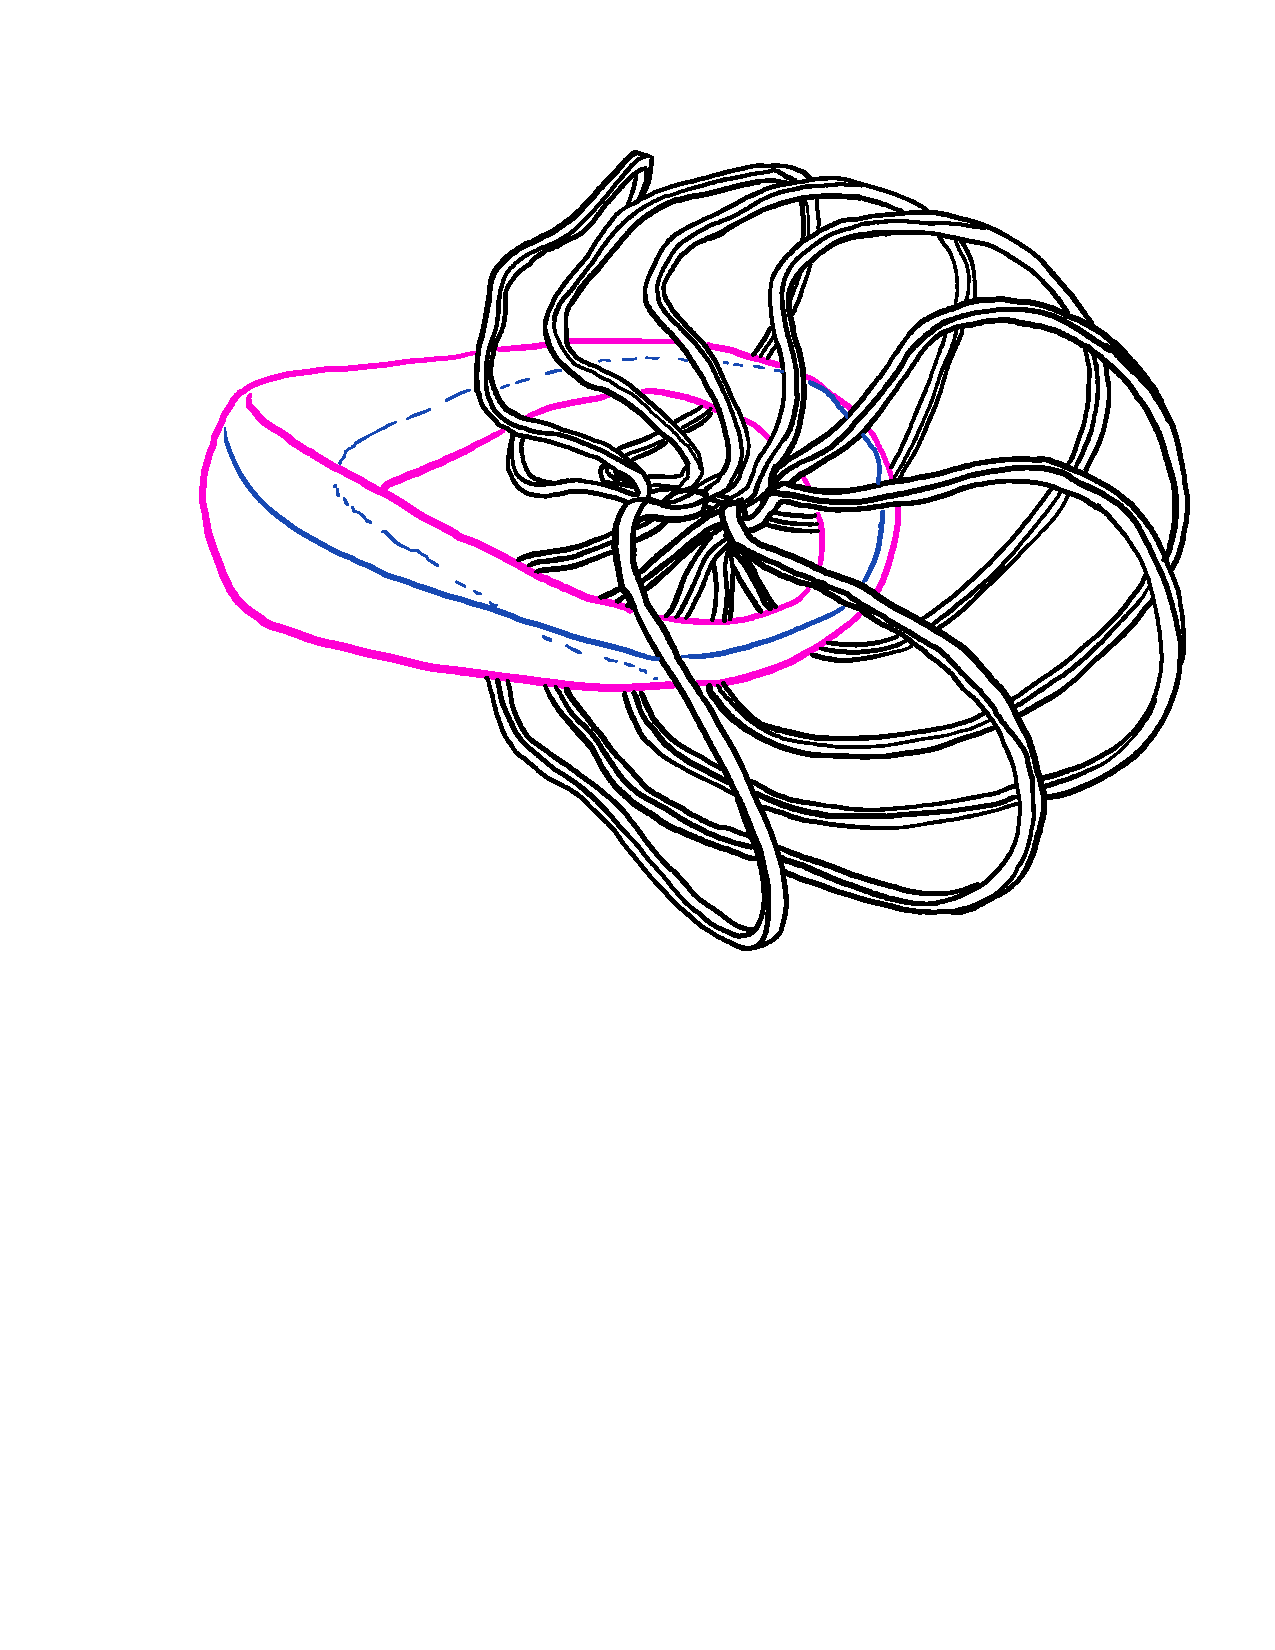
\includegraphics[width=0.6\textwidth]{3_chapters/0_introduction/img/stellarator-sketch.pdf}
    \caption{A sketch of a stellarator with half of all the coils drawn in black, the flux surface in purple, and a magnetic field line in blue. It can be seen that the complex three-dimensional shape can be achieved by having non-planar coils, which need to be constructed within tight tolerances. Based on \citet{wechsung2022precise}.}
    \label{fig: sketch stellarator}
\end{figure}



\section{Micro in scale, macro in consequences}
\label{sec: chap1 background}
Micro turbulence refers to turbulence which takes place on the scale of the gyroradius, which in tokamaks and stellarators is on the order of centimetres. Compared to the size of the device itself (typically measured in metres), this scale is indeed small. However, such smallness does not imply that one can safely ignore it.  Indeed, this microscopic turbulence is the main contributor to heat loss in current tokamaks and optimised stellarators, and we ought to understand it better if we are to make nuclear fusion power plants a reality. \par  

To deepen our understanding, let us make a distinction between neoclassical and turbulent transport, as the former can play an important role in some situations. There are many accounts available on neoclassical transport \cite{galeev1979reviews,kovrizhnykh1984energy,mynick2006transport,beidler2011benchmarking}, and therefore we shall only focus on the high-level understanding. A further distinction is made between neoclassical transport in stellarators and tokamaks, as they can be quite distinct. Let us start by focussing on the latter.

\subsection*{Neoclassical transport in stellarators}
In general (unoptimized) stellarators the dominant transport is neoclassical, due to the radial drift of particles, i.e. particles that drift across flux surfaces result in energy and density being transported across the device. If one wishes to insulate the hot core from the cool edge of the device, this is evidently problematic. As it turns out, trapped particles are the most problematic subset of species, as they may sample particularly deleterious regions of significant radial drift alone, whereas the passing particles benefit from sampling a flux-surface average. For stellarators, a pressing goal is thus to minimise the radial drift trapped particles experience, aiding in reducing the transport. Tokamaks do not suffer from the same problem, as their axisymmetry automatically implies that trapped particles do not drift radially, a result often called \textit{Tamm's theorem.} \par 
It is in attaining the favourable property of radially stationary trapped particles that we find foundational topics of stellarator physics. Indeed, the work is so central to the field that its pioneers, Alan Boozer and J\"urgen N\"uhrenberg, were awarded the Hannes Alfv\'en Prize in 2010 for their contributions made \cite{mendoncca201037th}. The findings enabled the community to reduce the neoclassical transport in stellarators to levels comparable to those of a tokamak \cite{landreman2022magnetic,paul2022energetic,goodman2022constructing}, and this reduced neoclassical transport has resulted in greatly improved performance in stellarators (see, e.g. Ref. \cite{beidler2021demonstration}). Let us next turn our attention to the neoclassical transport in tokamaks, so that we may better understand and quantify this transport.

\subsection*{Neoclassical transport in tokamaks}
To make statements about transport, it is useful to quantify it by means of a diffusion coefficient, denoted as $D$. This coefficient of some Brownian ``random walk'' process may be estimated as
\begin{equation*}
    D = \Delta r^2/\tau,
\end{equation*}
where $\tau$ is a typical timescale at which steps of the random walk are taken, and $\Delta r$ is the step-size of the walk. A simple estimate of this diffusion coefficient for a magnetised plasma can be derived in the following manner. \par 
The typical step-size perpendicular to the field will be the gyroradius $\rho$, and the time scale at which such steps are taken is the collision frequency. Focussing on energy transport, collisions of particles with similar mass lead to this transport.\footnote{This may be verified by investigating the limit case where one particle is much heavier than the other one. This scenario is like throwing a tennis ball against a wall; the tennis ball imparts a negligible amount of energy to the wall.} Let us estimate this collision frequency as follows; for Coulomb interactions to affect the particle trajectory, the kinetic and Coulomb energy should be of similar magnitude, i.e.
\begin{equation*}
    \frac{E_{\rm C}}{E_{\rm kinetic}} = \frac{\frac{1}{4\pi \epsilon_0} \frac{(Ze)^2}{r_{\rm C}} }{\frac{1}{2} m v^2} \approx 1 \implies r_{\rm C} \approx \frac{(Ze)^2}{2 \pi \epsilon_0 m v^2}.
\end{equation*}
Therefore, if the particles come within a distance $r_{\rm C}$ of each other, the Coulomb potential can significantly alter the trajectory. Now, the collision frequency may be estimated as $\nu_{\rm C} \sim n \pi r_{\rm C}^2 v$, and taking the velocity to be thermal ($v \sim \sqrt{T/m}$) we find
\begin{equation*}
    \tau_{\rm C} \sim  \frac{1}{\nu_{\rm C}} \sim \frac{\epsilon_0^2 m^{1/2} T^{3/2}}{n (Ze)^2}.
\end{equation*}
Let us combine the gyroradius and collision time to estimate the diffusion coefficient
\begin{equation}
    D_{\rm C} = \frac{\rho^2}{\tau_{\rm C}} \sim \frac{n}{\epsilon_0^2 B^2} \sqrt{\frac{m}{T}},
\end{equation}
and the scaling with mass implies that ions will be the dominant contributor to energy transport. A rigorous derivation is given by \citet{braginskii1958transport}, giving rise to the same scaling. Using typical values for the various parameters, one finds $D_{\rm C} \approx 10^{-3} \: {\rm m^2/s}$ \cite[p.~465]{freidberg2008plasma}. \par 
This classical estimate of heat diffusion is too optimistic, however, as step size and collision frequency increase in toroidal devices \cite[Ch.~7]{helander2005collisional}. This is due to trapped particles, which in tokamaks deviate from the flux surfaces by a ``banana width'' $\Delta r_{\rm b} \sim \frac{\rho}{\iota} \sqrt{R_0/a} $, with $a$ and $R_0$ being the minor and major radius of the torus, respectively. The collision time is reduced by the fact that changing the trajectory from trapped to untrapped is sufficient to make a step of banana width, changing the collision time by $\tau_{\rm b} = \tau_{\rm C}/(a/R_0)$. The diffusion coefficient is somewhat decreased due to the fact that only trapped particles contribute to it, reducing it by a factor $\sqrt{2 a /R_0}$. All in all one finds that this ``neoclassical'' estimate of the diffusion coefficient, which accounts for the trapped particles, is
\begin{equation}
    D_{\rm b} \sim \frac{(R_0/a)^{3/2}\sqrt{2} }{\iota^2} D_{\rm C},
\end{equation}
where the prefactor is of order $100$. Taking into account this trapped particle behaviour, we thus find $D_{\rm b} \approx 10^{-1} \: {\rm m^2/s}$. However, this estimate is still too optimistic compared to the experiments, and the discrepancy is attributed to turbulence.

\subsection*{Turbulent transport}
\begin{figure}[!b]
  \centering
  \subfloat[Prior to H-mode]{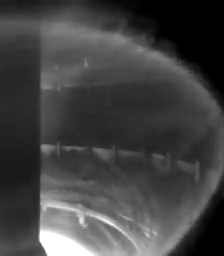
\includegraphics[width=0.4\textwidth]{3_chapters/0_introduction/img/pre-H-mode.png}}
  \hfill
  \subfloat[In H-mode]{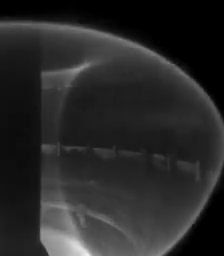
\includegraphics[width=0.4\textwidth]{3_chapters/0_introduction/img/H-mode.png}}
  \caption{The MAST tokamak prior to and in H-mode. Taken from shot \#29742 of the M9 campaign.}
  \label{fig: L-H mode in MAST}
\end{figure}
In magnetic confinement fusion devices, the step size is not determined by the gyroradius alone, but by turbulent fluctuations in the electric field as well.\footnote{Fluctuations in the magnetic field contribute too, but we ignore such effects here.} Such fluctuations will kick the particles around, causing them to be transported across flux surfaces, and we may estimate its magnitude as follows. The drifting velocity of particles due to an electric field may be estimated as $v_E \sim \nabla \phi/B$, where the electric potential satisfies $\boldsymbol{E} = - \nabla \phi$. If we then impose that the transport is local (i.e. it takes place on the scale of the gyroradius and is thus micro-turbulence), the step-size and spatial variation in $\phi$ are of order $\rho$, resulting in
\begin{equation}
    D_{\rm turb} \sim \frac{\rho \nabla \phi}{B} \sim \frac{T}{qB} \times \left( \frac{q\phi}{T} \right),
\end{equation}
The factor in brackets denotes the ratio of the potential energy of the particle and the temperature, and this electrostatic potential is determined by the turbulence. Its dependencies are crucial to understanding how transport in turbulent systems behaves, and the main idea of this thesis is to find a method of estimating the magnitude of this quantity. To put a number to this turbulent transport, in experiments it is typically found that $D \approx 1 \: {\rm m^2/s}$, roughly an order of magnitude higher than our estimate using trapped particles.
\par 

To sketch the effects this increased diffusion coefficient has on the performance of our reactor, one can investigate situations in which this anomalous transport is largely suppressed. In tokamaks, this is the case in the so-called H-modes, in which there exists a steep pressure gradient at the edge of the reactor \cite{itoh1988model,burrell1992physics,groebner1993emerging,burrell2005advances}. Such an H-mode is characterised by a reduction in transport, making it possible to maintain a steep pressure gradient. This reduction in transport brings with it such benefits that many tokamak power plant scenarios now assume H-mode operation to achieve the conditions required. A figure showing the transition to H-mode in MAST is shown in Fig. \ref{fig: L-H mode in MAST}. \par 

As we have seen, a deeper understanding of micro-turbulence is highly sought after as it may help us reach improved reactor performance. This is true for both tokamaks and stellarators, where the latter have a much larger configuration space, which may help in reaching reduced micro-turbulence. However, since the flowing plasma creates electromagnetic fields affecting its own flow, the process is nonlinear. In a mathematical sense, this disallows us from decomposing the solution space into simpler independent constituents (e.g. Green's functions or Fourier modes), hindering analysis. Physically, this non-linear behaviour manifests itself as multiple instabilities that interact with each other, which can cause predator-prey-like dynamics \cite{morel2013characterization}. In tokamaks and stellarators the turbulence is well described by the gyrokinetic equations, and these equations take centre stage for micro-turbulence investigations.

\subsection*{The gyrokinetic equations}
\label{subsec: Gyrokinetic equations}
There exist a number of resources that derive the gyrokinetic equations in different ways \cite{dubin1983nonlinear,hahm1988nonlinear,brizard2007foundations,parra2011phase,krommes2012gyrokinetic,burby2015hamiltonian}, and we shall not focus too much on such specifics here and instead focus on the main concepts and difficulties involved. In general, in plasma kinetics one is interested in solving a Boltzmann equation (which is a continuity equation) of the form
\begin{equation}
    \frac{\mathrm{d} f_s}{\mathrm{d} t} \equiv \frac{\partial f_s}{\partial t} + \boldsymbol{v} \cdot \nabla_{\boldsymbol{r}} f_s + \frac{\boldsymbol{F}}{m} \cdot \nabla_{\boldsymbol{v}} f_s = \mathrm{sources/sinks/collisions},
\end{equation}
where $f_s(t,\boldsymbol{r},\boldsymbol{v})$ is the plasma distribution function of species $s$, $t$ is the time, $\boldsymbol{r}$ is the position vector, $\boldsymbol{v}$ is the velocity vector, $\boldsymbol{F}$ is the force acting on the particles, and we have made use of Feynman subscript notation for the divergence. The right-hand side of the above equation encapsulates sources and sinks of particles, energy, or momentum, which may consist of collisions with other species and external actuators. \par 

In fusion-relevant conditions, the electromagnetic force typically dominates, meaning that one may take the Lorentz force
\begin{equation}
    \boldsymbol{F} = q \left( \boldsymbol{E} + \boldsymbol{v} \times \boldsymbol{B} \right).
\end{equation}
It is crucial to realise that a non-linearity enters here: since the plasma consists of charged particles, it generates its own electromagnetic fields, making $\boldsymbol{E}$ and $\boldsymbol{B}$ dependent on $f$. This non-linearity hinders straightforward mathematical analysis. We are somewhat helped by the fact that, under fusion-relevant conditions, collisions can often be neglected, as the collision frequency scales as $T^{-3/2}$, with $T$ being the plasma temperature. Hence, at the extreme temperatures present in fusion-relevant conditions, collisions become rare and may be neglected,\footnote{An excellent counter-point is that, if collisions are negligible, how is fusion to happen? More formally, it turns out to be a matter of time scales, i.e. collisions happen much less often than typical frequencies associated with the micro-turbulence and the turbulence can saturate without feeling the effects of the collisions \cite{garbet2010gyrokinetic}. However, this assumption is not always valid and collisions affect turbulence in some situations \cite{rewoldt1990toroidal,lin1999effects,falchetto2004effect,morren2022influence}. In certain systems, important differences can arise if one takes the collisionless limit instead of neglecting collisions all together, essentially due to the mathematical fact that $\lim_{\mathrm{x \rightarrow a}} f(x) \neq f(a)$ in general: see \citet{ng2021landau} for a pertinent example.} rendering this equation somewhat simpler. Other sources and sinks (e.g. electron cyclotron resonance heating or pellet injection) should in general be taken into account but are ignored here. \par

This simplified form with neglected collisions, sources, and sinks is called the \textit{Vlasov equation,} and it has several properties of interest. Importantly, the Vlasov equation has a Liouville theorem (i.e., phase-space flow incompressibility) and an action principle for both electromagnetic fields and particles \cite{landau2013classical}. We may simplify this action once more by expanding the Vlasov equation around a small parameter $\delta$, where $\rho/L\sim \omega/\Omega_{\rm ions} \sim q \phi / T \sim \delta $, with $L$ denoting a global length scale (e.g. minor radius), $\omega$ denoting frequencies of interest and $\Omega_{\rm ions}$ denoting the ion gyration frequency. This expansion, combined with the gauge freedom of the action, allows us to find a reduced set of equations (see \citet{scott2017gyrokinetic}). The resulting reduced set of equations is the gyrokinetic equations and its phase-space dimensionality is lower one degree lower than the Vlasov equation (i.e. 5 dimensions instead of 6). The ``neglected'' dimension turns out to be the so-called gyrophase, the phase of a particle gyrating around a magnetic field line (a sketch may be seen in Fig. \ref{fig: gyrophase sketch}). The reason why it may be neglected makes physical sense as well: in the limit of strong magnetic fields where $\omega/\Omega_{\rm ions} \sim \delta$, the gyration frequency is much larger than other time scales of relevance, meaning that it can be safely ignored. \par
\begin{figure}
    \centering
    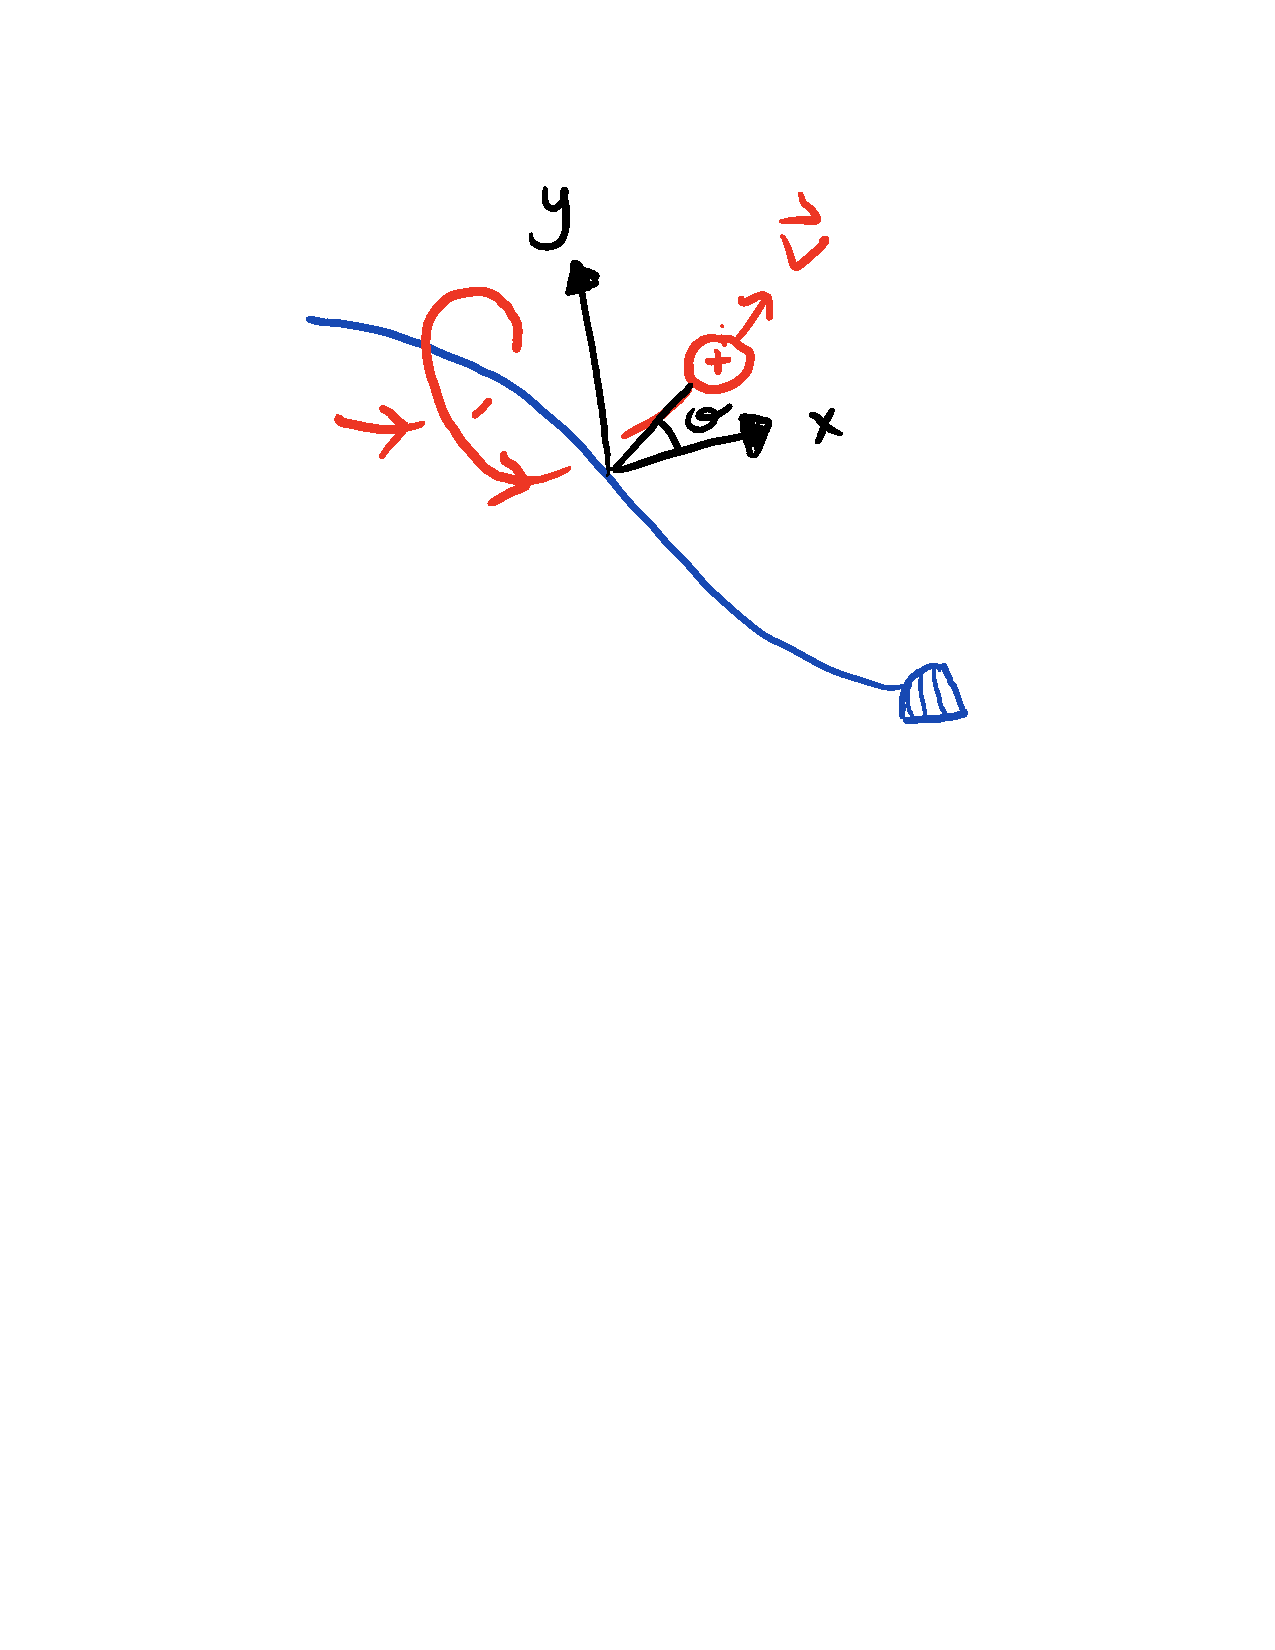
\includegraphics[width=0.5\textwidth]{3_chapters/0_introduction/img/gyrophase-sketch.pdf}
    \caption{A sketch of a positively charged particle's path in red, as it gyrates around a magnetic field line in blue. The helical path has a certain gyrophase associated with it at every location, denoted as $\vartheta$.}
    \label{fig: gyrophase sketch}
\end{figure}

Although this set of equations constitutes a reduced model, it is still computationally very demanding to solve. There are multiple codes available which solve these equations (where some use various additional assumptions on the magnetic geometry; see Refs. \cite{jenko2000electron,barnes_michael_2022_6882296,maurer2020gene,barnes2019stella,francisquez2020gkeyll} for a non-exhaustive list), but computations can still typically take $\gtrsim 10^5$ CPU-hours.\footnote{It should be noted that this is a rapidly evolving field, with large strides being made by the year. For example, by using fully spectral methods on GPUs certain calculations have been cut down by orders of magnitude \cite{mandell_dorland_landreman_2018,mandell2022gx}.} Millions of lines of code (a count of a couple codes brings me to a total of 2288153 lines) and some hundred thousand man-hours have been put into this development, and the extremely thorough numerical analysis by the community has brought with it great insight. One particularly pressing insight is that when equilibrium parameters are changed slightly (e.g., magnetic shear, ratio of thermal to magnetic pressure, geometry), the micro-turbulence may change greatly \cite{dimits2000comparisons,kinsey2006effect,alcuson2020suppression,volvcokas2022ultra,mulholland2023enhanced}. As such, each new point in parameter space should be carefully simulated before we can make statements about them. This raises the question: is there anything we can say about these equations {\it in general?} Are there fundamental properties of the Vlasov and gyrokinetic equations that can estimate the magnitude of turbulence?

\section{Available energy}
There are indeed fundamental properties that one can exploit to make general statements if the system is Hamiltonian and thus satisfies Liouville's theorem. This boils down to the fact that the dynamics of such a system inhabits a constrained subspace in the set of all distribution functions. The set of accessible distribution functions is set by the initial distribution function $f_i \equiv f(t=0)$, and we denote the total set $\mathcal{F}_L$ (where the subscript denotes that the space is constrained via Liouville's theorem) as
\begin{equation}
    f(\boldsymbol{x},t) \in \mathcal{F}_L [f_i]; \; \forall t \geq 0.
    \label{eq:set-of-all-distribution-functions}
\end{equation}
We may furthermore associate a total thermal energy to each distribution function, which is simply
\begin{equation}
    E_T[f] \equiv \int \epsilon f(\boldsymbol{x},t) \mathrm{d} \boldsymbol{x},
\end{equation}
where $\epsilon$ is the particle energy (typically $\epsilon=mv^2/2$).\par 
A natural question to ask oneself given these concepts is the following: \textit{what is the minimiser of the thermal energy in the set of accessible distribution functions?} In a more mathematical sense, we wish to find the function $f_0$, which satisfies
\begin{equation}
    f_0 \equiv \argmin_{f \in \mathcal{F}_L[f_i]} \:  E_T[f].
\end{equation}
This minimiser of the thermal energy is called the ground state, and this quantity will play a central role in the current thesis. It is a quantity of relevance because the Vlasov equation (for certain boundary conditions) conserves the total energy, which is the sum of the energy in the electromagnetic field and the thermal energy. Hence, if one loses thermal energy, this energy has to be transferred to the electromagnetic field, which, in turn, may drive instabilities. If one starts out with a state in which there is no energy in the electromagnetic field, we can thus construct an upper bound for the total energy that can possibly reside in it. It is this upper bound that we shall call the \textit{available energy}, which shall be abbreviated to \AE{}, and it is formally defined as
\begin{equation}
    A = E_T[f_i] - E_T[f_0] \geq 0,
\end{equation}
where the available energy $A$ is always greater than or equal to zero by definition.
\begin{figure}
    \centering
    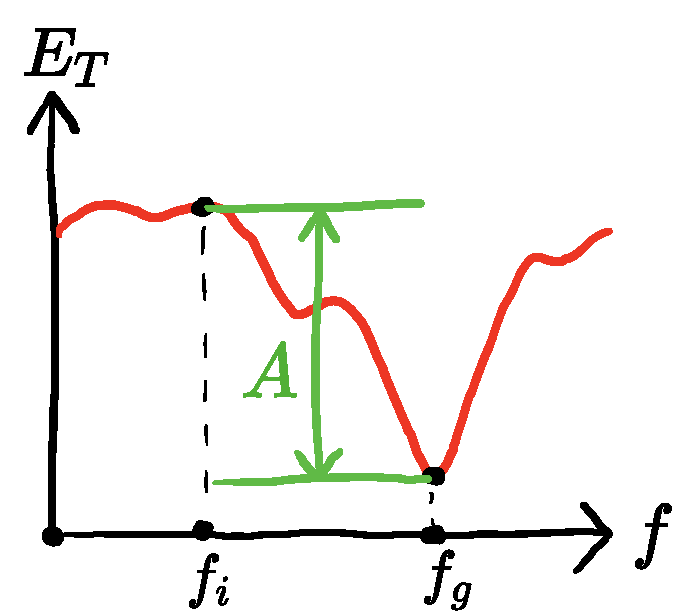
\includegraphics[width=0.5\textwidth]{3_chapters/0_introduction/img/AE-def.pdf}
    \caption{A pictorial representation of the \AE{}. The $x$ axis contains the distribution functions $f \in \mathcal{F}_L$, and the $y$ axis is their associated thermal energy. The initial distribution function is denoted by $f_i$ and the ground state is denoted by $f_g$. Finally the available energy is denoted in green as $A$.}
    \label{fig: ae def}
\end{figure}
We finally include a pictorial representation of the \AE{} in Fig. \ref{fig: ae def}, where one can see that the \AE{} is defined as the difference in energy between the initial distribution function and the ground state.
\subsection*{History \& development of the concept}
The concept of \AE{} and its mathematical equivalents have been known since 1930. In that year, \citet{riesz1930inegalite} employed an equivalent concept to derive certain integral inequalities, and such Riesz–Sobolev inequalities remain an active field of mathematical research \cite{burchard1996cases,burchard2006rearrangement,hajaiej2011necessity,carlen2017stability,frank2019proof}. The concept first entered the field of physics in 1955, where \citet{lorenz1955available} calculated the \AE{} of the atmosphere under an adiabatic rearrangement. Eight years later, \citet{gardner1963bound} recognised the relevance of such concepts for plasma physics and derived the \AE{} of a collisionless plasma. It will be of interest to note that Gardner's research focused on the \AE{} of a plasma that is subject to Liouville's theorem {\it alone,} i.e. there are no additional constraints on the system. Gardner was acutely aware of this important distinction, as he explicitly points it out in the abstract of his aforementioned paper. \par 
Though this distinction was recognised in 1963 by Gardner, it was \citet{helander2017available,helander2020available} who recognised its significance in 2017. By allowing additional constraints on the set of accessible distribution functions, the \AE{} becomes relevant to magnetically confined plasmas, as such plasmas do not obey Liouville's theorem alone; they have additional {\it adiabatic invariants.} If we denote an additional set of conserved invariants by $\boldsymbol{y}$, the set of accessible distribution functions is thus reduced by constancy of these invariants, and this set shall be denoted by $\mathcal{F}_L[f_i;\boldsymbol{y}]$.\footnote{Note that $\mathcal{F}_L[f_i;\boldsymbol{y}] \subseteq \mathcal{F}_L[f_i]$, which implies that the \AE{} with constancy of adiabatic invariants is smaller than or equal to the \AE{} without such constancy.} Helander employed an elegant scheme (involving Lagrange multipliers) to find the ground-state of such plasmas, and was able to reproduce many known results from the literature. \par 
All mentioned research has relied heavily on Liouville's theorem, and it is natural to wonder how breaking of this theorem affects \AE{}. It, very surprisingly, turns out that \AE{} in continuous systems which allow for phase-space mixing is the \textit{same} is in systems in which Liouville's theorem is obeyed, as proven in \citet{kolmes2020recovering} in 2020. In terms of collisionality, \AE{} is thus unchanged as one increases the collision frequency given that the adiabatic invariants $\boldsymbol{y}$ remain conserved. There is an additional question, pertaining to accessibility of ground state. That is, though the ground state is within the set of distribution functions obeying certain conditions, it is not guaranteed that the ground state is {\it dynamically accessible,} and some comments relating to dynamical accessibility of ground states may be found in \citet{ewart2022collisionless}.\footnote{In general one should not expect the ground state to be accessible (best surmised by A. Schekochihin, who during a talk cleverly remarked ``\textit{the bound is bound not to be sharp}''). This is because we have not imposed that this ground state supports an electromagnetic field which has the appropriate magnitude. This ailment can be remedied, and in simplified scenarios this difference turns out to be minute. More general scenarios are still being considered in a collaboration with R.J. Ewart} More generally, since it is unknown whether the state is accessible \textit{a priori} one can best interpret \AE{} as an upper bound of the amount of liberated thermal energy. 
\section{Research question \& contributing works}
Given the generality of the concept of \AE{}, it is somewhat surprising that it has found fairly little use as a practical tool to study gyrokinetic turbulence in fusion reactors. This is especially true given the fact that \AE{} possesses the following attractive properties:
\begin{enumerate}
    \item It provides a natural mapping from the magnetic geometry of the device (i.e. the shape of the flux-surfaces) and the plasma profiles (e.g. pressure and temperature) to a scalar. This allows one to condense the large parameter space of fusion reactors into a physically meaningful quantity.
    \item Although the calculation of \AE{} in the most general case is not trivial, it can be significantly faster than the gyrokinetic codes. This is partly a consequence of the fact that \AE{} is not a dynamical quantity; there is no time-stepping involved.
    \item Vanishing \AE{} (that is, $A = 0$) implies \textit{ nonlinear} stability. Thus, it is natural to quantify the distance from such stability thresholds.
\end{enumerate}
We note in passing that these factors not only make \AE{} interesting as a measure of turbulence but also make it interesting as an optimisation measure. Overall, given the broad applicability and relatively unexplored use of \AE{} in gyrokinetic turbulence, the central idea of the current thesis is the following:
\boxedtext{Can \AE{} predict gyrokinetic turbulent transport and can it be used to infer its dependencies?}

Since \AE{} is a very broadly applicable, we choose to specialise in trapped-electron-mode driven turbulence first, and its corresponding \AE{}. As it turns out, many quantities signifying trapped particles will enter into the calculation of the \AE{}, and we first develop numerical methods of evaluating these quantities efficiently, which is the first contribution of this thesis.
\itemheader{Bounce-averaged drifts: equivalent definitions, numerical implementations, and example cases}
\textit{Abstract:} In this paper, we provide various analytical and numerical methods for calculating the average drift of magnetically trapped particles across field lines in complex geometries, and we compare these methods with each other. To evaluate bounce-integrals, we introduce a generalisation of the trapezoidal rule, which is able to circumvent integrable singularities. We contrast this method with more standard quadrature methods in a parabolic magnetic well and find that the computational cost is significantly lower for the trapezoidal method, though at the cost of accuracy. With numerical routines in place, we next investigate conditions on particles which cross the computational boundary, and we find that important differences arise for particles affected by this boundary, which can depend on the specific implementation of the calculation. Finally, we investigate the bounce-averaged drifts in the optimized stellarator NCSX. From investigating the drifts, one can readily deduce important properties, such as what subset of particles can drive trapped-particle modes, and in what regions radial drifts are most deleterious to the stability of such modes.
\contribution{Develop new numerical methods for evaluating the bounce-averaged drift, and develop benchmark cases to test them on. Finally, recognize that the computational boundary may affect the trapped-particle drift in non-trivial ways.}{\label{contr:BAD}} \par 
The second contribution employs these numerical methods to find the \AE{} of trapped electrons. To this end, we derive the \AE{} of trapped electrons to non-omnigenous systems, which generalizes results found in \citet{helander2020available}, and we go on to investigate it in some depth. Importantly, we compare \AE{} against the nonlinear heat-flux, an important measure for turbulence in magnetic confinement fusion reactors. 
\itemheader{The available energy of trapped particles and its relation to turbulent transport} \\
\textit{Abstract:} A collisionless plasma possesses a certain amount of ``available energy'', which is that part of the thermal energy that can be converted into kinetic energy of plasma motion and electromagnetic fluctuations. In this paper we present a calculation of the available energy carried by trapped electrons in a slender non-omnigenous flux tube of plasma. This quantity is compared with gyrokinetic simulations of the nonlinear saturated radial energy flux resulting from turbulence driven by collisionless trapped-electron modes in various stellarators and a tokamak. The numerical calculation of available energy is fast and shows a strong correlation with the turbulent energy fluxes found in the gyrokinetic simulations. Indeed, the energy flux is found to be proportional to the available energy to the power of approximately $3/2$, which is what one would expect from a simple argument. We furthermore investigate how available energy is distributed across different bounce wells, and it is found that deeply trapped electrons typically contribute most to the available energy. Finally, we investigate the dependence of available energy on gradient strength, and we find important differences between weakly and strongly driven regimes for stellarators and tokamaks.
\contribution{Generalize the \AE{} of trapped particles to account for non-omnigenous systems. Develop numerical routines to calculate the \AE{}. Relate \AE{} to turbulent transport. Investigate which regions are most unstable, and investigate how the \AE{} changes with gradient strengths.}{\label{contr:AE-and-turbulence}}

Seeing the found utility of the \AE{} of trapped electrons, we go on to specialise to tokamaks, which we parameterize via the Miller equilibrium \cite{miller1998noncircular}. The model allows us to make statements about the possible benefits and disadvantages of negative triangularity tokamaks, which have found renewed interest after having shown improved confinement in such cases \cite{marinoni2021brief}. Triangularity is a measure in tokamaks of how triangular the flux-surfaces are, and negative/positive triangularity have the triangle pointing towards/away from the center of the torus. We go in to investigate how \AE{} against a number of other equilibrium parameters, and find that it is able to reproduce many trends.

\itemheader{Available energy of trapped electrons in Miller
tokamak equilibria} \\
\textit{Abstract:} Available energy (\AE{}), which quantifies the maximum amount of thermal energy that may be liberated and converted into instabilities and turbulence, has shown to be a useful metric for predicting saturated energy fluxes in trapped-electron-mode-driven turbulence. Here, we calculate and investigate the \AE{} in the analytical tokamak equilibria introduced by \citet{miller1998noncircular}. The \AE{} of trapped electrons reproduces various trends also observed in experiments; negative shear, increasing Shafranov shift, and negative triangularity can all be stabilizing as indicated by a reduction in \AE{}, though it is strongly dependent on the chosen equilibrium. We find that negative triangularity is especially beneficial in vertically elongated configurations with positive shear, or low gradients. We furthermore extract a gradient-threshold like quantity from \AE{} and find that it behaves similarly to gyrokinetic gradient-thresholds: it tends to increase linearly with magnetic shear, and negative triangularity leads to an especially high threshold. We next optimize device geometry for minimal \AE{} and find that the optimum is strongly dependent on equilibrium parameters. If one furthermore investigates the competing effects of increasing the density gradient, pressure gradient, and decreasing the shear, one finds regimes which have steep gradients yet low \AE{}, and that the existence of such a regime is inaccessible in negative-triangularity tokamaks. We finally compare \AE{} with saturated heat-flux estimates from the \textsc{tglf} model and find fairly good correspondence.

\contribution{Investigate possible benefits/disadvantages of negative triangularity. Find dependencies of an critical gradient-like quantity in \AE{}. Research how geometrically \AE{}-optimized tokamaks depend on equilibrium parameters. Investigate how \AE{} differs as one enters a pedestal-like regime. Finally, compare against \AE{} against heat-fluxes from \textsc{tglf}.}

\section{Outline of the thesis}
[To be filled in after finalisation of the structure.]
% \section{Scrap}
% \label{sec: chap1 contributions}

% Supposing that one parameterizes phase-space by the coordinates $\boldsymbol{x}$, which furthermore have the Jacobian $\sqrt{g}$, the continuity equation for the particle distribution function becomes
% \begin{equation}
%     \frac{\partial (f\sqrt{g})}{\partial t} + \dot{\boldsymbol{x}} \cdot  \nabla_{\boldsymbol{x}} (f\sqrt{g}) = 0.
%     \label{eq: continuity equation in general}
% \end{equation}
% Now, phase-space incompressibility implies that the Jacobian obeys
% \begin{equation}
%     \frac{\partial \sqrt{g}}{\partial t} + \dot{\boldsymbol{x}} \cdot \nabla_{\boldsymbol{x}} \sqrt{g} = 0.
%     \label{eq: Liouville theorem for Jacobian}
% \end{equation}
% Combining Eqs. \eqref{eq: continuity equation in general} and \eqref{eq: Liouville theorem for Jacobian}, we find
% \begin{equation}
%     \frac{\partial f}{\partial t} + \dot{\boldsymbol{x}} \cdot \nabla_{\boldsymbol{x}} f = 0.
% \end{equation}
% If we now multiply the above equation by some function $G'[f]$, use the chain rule, and finally integrate over $\boldsymbol{x}$, one finds
% \begin{equation}
%     \frac{\mathrm{d}}{\mathrm{d} t} \int G[f] \mathrm{d} \boldsymbol{x} = 0 \longrightarrow \int G[f] \mathrm{d} \boldsymbol{x} = \mathrm{const.}
%     \label{eq: constraints G[f]}
% \end{equation}
% Eq. \eqref{eq: constraints G[f]} puts an uncountably infinite number of constraints on $f$, as we may choose any well-behaved function $G[f]$. In essence, this equation describes Liouville's theorem from the perspective of the distribution function: since phase-space flow is incompressible, the set of all $f$ is heavily constrained. To gain some insight we parameterize the functions $G[f]$ as
% \begin{equation}
%     G[f] = H[f-\phi]; \quad \forall \phi \in \mathbb{R},
% \end{equation}
% where $\phi$ is some scalar constant and $H[x]$ is the Heaviside function of $x$. To aid notation, denote this constrained subset of distribution functions as $\mathcal{F}[f_i]$ where the member distribution functions $f$ of this set are defined by
% \begin{equation}
%     \int H[f - \phi] \mathrm{d} \boldsymbol{x} = \int H[f_i-\phi]\mathrm{d} \boldsymbol{x} ; \; \forall \phi \in \mathbb{R} \iff f \in \mathcal{F}[f_i].
% \end{equation}
% Here $f_i\equiv f(t=0,\boldsymbol{x})$ is the initial condition/distribution function, which determines the set of accessible distribution functions. Summarizing, one finds that, if there is a continuity equation for $f$ with a Liouville theorem, $f \in \mathcal{F}[f_i]$ where $f_i$ is the initial condition. \par 

% Let us use this knowledge to our benefit.

% %**********************************************************************%

% \itemheader{Topic 1}
% \lipsum[1-2] This leads to the first contribution of our work:

% \contribution{First contribution of your work.}{\label{contr: contribution 1}}

% Explain a bit more about your first contribution.

% %**********************************************************************%

% \itemheader{Topic 2}
% \lipsum[4-5] This leads to the second contribution of our work:

% \contribution{Second contribution of your work.}{\label{contr: contribution 2}}

% Explain a bit more about your second contribution.

% %**********************************************************************%

% \itemheader{Topic 3}
% \lipsum[1-2] The last contribution of the research thus is:

% \contribution{Third contribution of your work.}{\label{contr: contribution 3}}

% Explain a bit more about your third contribution.


% \section{Outline of the thesis}
% \label{sec: chap1 outline}

% \lipsum[10-12]

% \itemheaderNewpage{A note for the reader} Chapters~...-... are all based on submitted/published articles and consequently are self-contained and can be read independently. A reference to the corresponding research paper is included at the beginning of each chapter.
% An overview of how the chapters of this thesis relate to the contributions presented in Section~\ref{sec: chap1 contributions} is given in Table~...


\chapter[Theory]{Theory of trapped particles and \AE{}}
\label{chap: chapter 2}
Here, we set up the equations describing the central concepts that enter into the calculation of \AE{}.\footnote{This chapter highlights the central concepts given in references \cite{helander2005collisional,helander2014theory,helander2017available,helander2020available}.} The difficulty will be finding some way to parameterise the set given in Eq. \eqref{eq:set-of-all-distribution-functions}, especially if additional conserved quantities $\boldsymbol{y}$ are present. Using Liouville's theorem, we shall, however, be able to implicitly construct this set. More pressingly, however, is the choice of invariants considered, which we shall investigate first.


\section{Lagrangian mechanics and trapped particle orbits}
\label{sec: lagrangian mechanics and trapped particles}
As hinted at in the previous sections, trapped particles play a central role in the current thesis, and thus we highlight some important concepts required when investigating such particles. As it turns out, Lagrangian mechanics is the natural mathematical language for investigating such particles, and as such, we first start with a brief primer on these methods.
\subsection{Lagrangian mechanics}
In 1788, Joseph-Louis Lagrange, a French mathematician, wrote an elegant reformulation of Newtonian mechanics during his stay in Berlin \cite{lagrange1853mecanique}. The main benefit of the formalism carrying his name is that it is coordinate-independent, and it makes recognising certain conserved quantities trivial. The central concept in the formalism is the action, $\mathcal{S}$, which is the path integral of the Lagrangian $\mathcal{L}$,
\begin{equation}
    \mathcal{S} = \int \mathcal{L}(\boldsymbol{q}(t),\dot{\boldsymbol{q}}(t),t) \mathrm{d} t.
\end{equation}
Here, $\boldsymbol{q}$ and $\dot{\boldsymbol{q}}$ denote some arbitrary coordinate system and temporal derivatives thereof, and the Lagrangian is defined as the difference of the kinetic and potential energies, $\mathcal{L} = E_{\rm kinetic} - E_{\rm potential}$. We now seek to find a path $\boldsymbol{q}(t),\dot{\boldsymbol{q}}(t)$ that minimises the action, which may be found by introducing the addition of small variation $ \delta \boldsymbol{q}(t),\delta \dot{\boldsymbol{q}}(t)$ and imposing that the variation $\delta \mathcal{S}$ vanishes. This results in the Euler-Lagrange equation,
\begin{equation}
    \frac{\mathrm{d}}{\mathrm{d} t} \left( \frac{\partial \mathcal{L}}{\partial \dot{\boldsymbol{q}}} \right) = \frac{\partial \mathcal{L}}{ \partial \boldsymbol{q} }.
    \label{eq: EL equation}
\end{equation}
The above equation is exactly equivalent to Newton's equations of motion, but with the coordinate-system $\boldsymbol{q}$ chosen arbitrarily. If one furthermore finds that the Lagrangian depends only on $\dot{q}_i$ and \textbf{not} on $q_i$ we find that $\partial_{\dot{q}_{i}} \mathcal{L}$ is a conserved quantity. \par 
Herein lies the power of Lagrangian mechanics: find a well-chosen coordinate system $\boldsymbol{q}$, and one may readily derive constants of motion. In the next section, we specialise in the dynamics of charged particles, where we will encounter several such constants of motion. These will prove crucial when investigating \AE{}, and as such, let us carefully derive them.
\subsection{Charged particle dynamics and the first invariant}
To this end, let us first consider the Lagrangian of a (non-relativistic) particle in a magnetic field, which is given by \cite[Sec.~16]{landau2013classical}
\begin{equation}
    \mathcal{L} = \frac{1}{2} m v^2 + q\boldsymbol{A} \cdot \dot{\boldsymbol{r}},
\end{equation}
where $\boldsymbol{A}$ is the magnetic potential which satisfies $\nabla \times \boldsymbol{A} = \boldsymbol{B}$, and $q$ denotes the particle charge. One can expand this Lagrangian around the smallness of the gyroradius $\rho$ (more precisely, $\rho$ should be small compared with variations of the magnetic field), giving rise to the gyroaveraged Lagrangian. More specifically, the position vector $\boldsymbol{r}$ is split into a guiding centre and a gyrating component
\begin{equation}
    \boldsymbol{r} = \underbrace{\boldsymbol{R}}_{\text{guiding centre}} + \underbrace{\boldsymbol{\rho}}_{\text{gyration}},
\end{equation}
and takes $\boldsymbol{\rho}$ to be small. There are many accounts available of this expansion \cite{littlejohn1983variational,helander2005collisional,cary2009hamiltonian,rodriguez2022quasisymmetry}, and we refer to these references for detailed derivations. I shall simply state the result of this expansion, namely
\begin{equation}
    \overline{\mathcal{L}} \approx \frac{m}{2B}\left( \boldsymbol{B} \cdot \dot{\boldsymbol{R}} \right)^2 + q \boldsymbol{A} \cdot \dot{\boldsymbol{R}} + \frac{m(\rho \dot{\vartheta})^2}{2} + \frac{q \rho^2 \dot{\vartheta} B}{2}
\end{equation}
where $\vartheta$ is the angle of gyration. We first derive the Euler-Lagrange equation for $\dot{\vartheta}$, resulting in our first constant of motion (to the order of the expansion)
\begin{equation}
    \frac{\mathrm{d}}{\mathrm{d} t} \left( \frac{\partial \mathcal{L}}{\partial \dot{\vartheta}} \right) = \frac{\mathrm{d}}{\mathrm{d} t} \left( m \rho^2 \dot{\vartheta} + \frac{q B \rho^2}{2} \right) = 0.
    \label{eq: mu-cons general}
\end{equation}
To get this in a more familiar form, let us next investigate the Euler-Lagrange equation for $\rho$, resulting in
\begin{equation}
    \partial_\rho \overline{\mathcal{L}} = m \rho \dot{\vartheta}^2 + q \rho \dot{\vartheta} B = 0 \implies \dot{\vartheta} = -\frac{qB}{m} \equiv \Omega.
\end{equation}
Combining this with Eq. \eqref{eq: mu-cons general} we find that $\rho^2 \Omega$ is a conserved quantity. Finally realising that $\rho \Omega$ is simply the velocity perpendicular to the field line $v_\perp$, we find our desired constant of motion.
\begin{equation}
    \mu = \frac{m v_\perp^2}{2B}.
\end{equation}
Given an adequately magnetised plasma (i.e. $\rho$ should be small enough), $\mu$ is thus a conserved quantity. This will be one of the invariants that will be considered in the calculation of \AE{}. \par 
A crucial step in this derivation was finding a convenient coordinate system to express the Lagrangian in, which is where the guiding centre decomposition of the coordinate $\boldsymbol{r}$ entered. If we express $\boldsymbol{R}$ in terms of a convenient coordinate system once more, we shall find an additional constant of motion for trapped particles. The existence of such trapped particles can be readily seen as follows; first consider a point particle of mass $m$ attached to a rigid wire whose height is described by $h(x)$, in a gravitational field with constant acceleration $g$. The total energy may thus be written as the sum of the kinetic and potential components,
\begin{equation}
    E = \frac{1}{2}mv^2 + mgh(x).
\end{equation}
Compare this with the total energy of a particle in a magnetised plasma,
\begin{equation}
    E = \frac{1}{2}mv_\parallel^2 + \frac{1}{2}mv_\perp^2 = \frac{1}{2}mv_\parallel^2 + \mu B.
\end{equation}
Seeing the correspondence between the two energies, one sees that $\mu B$ can be interpreted as an effective ``potential.'' In fact, if we write down a Lagrangian with this potential, $\mathcal{L} = mv_\parallel^2/2 - \mu B$, the Euler-Lagrange equation for the parallel coordinate becomes
\begin{equation}
    m \dot{v}_\parallel = - \mu \nabla_\parallel B,
\end{equation}
and we have derived the so-called ``mirror force.'' This mirror reflects particles as they try to enter regions of stronger magnetic field. The point where the mirror force changes the sign of $v_\parallel$ is called the ``bounce point'', which, from energy considerations, must satisfy $E = \mu B$. Of further interest is the perpendicular dynamics of these trapped particles, and these dynamics are readily derived in Clebsch coordinates; the focus of the next section.

\subsection{A brief intermezzo on Clebsch coordinates}
The convenient choice of coordinates turns out to be the so-called Clebsch coordinates, which we briefly review here (one may refer to \citet{d2012flux} for a more complete overview, and this section follows Ref. \cite{helander2014theory}). Assuming that one satisfies magnetohydrodynamic equilibrium conditions, $\boldsymbol{J} \times \boldsymbol{B} = \nabla  p$ (with $\boldsymbol{J}$ being the current density), the magnetic field in toroidal geometry may be written as
\begin{equation}
    \boldsymbol{B} = B_1(p,\theta,\phi) \nabla p \times \nabla \theta + B_2(p,\theta,\phi) \nabla \phi \times \nabla p.
\end{equation}
Here, $\theta$ and $\phi$ are arbitrary angles that parameterise a surface of the torus, $p$ is the pressure, and $B_1$ and $B_2$ are functions we wish to find. In this form, we have ensured that $\boldsymbol{B} \cdot \nabla p = 0$, as required by the equilibrium conditions. We furthermore require that the magnetic field be divergence-free, i.e. $\nabla \cdot \boldsymbol{B} = 0$, which results in 
\begin{equation}
    \left( \frac{\partial B_1}{\partial \phi} + \frac{\partial B_2}{\partial \theta} \right) \nabla p \cdot \left( \nabla \theta \times \nabla \phi \right) = 0 \implies \frac{\partial B_1}{\partial \phi} + \frac{\partial B_2}{\partial \theta} = 0.
\end{equation}
As such, $B_1$ and $B_2$ can in general be represented as 
\begin{subequations}
\begin{alignat}{4}
B_1 &= \partial_\theta f + g(p), \\
B_2 &= \partial_\phi f   + h(p).
\end{alignat}
\end{subequations}
for some functions $f(p,\theta,\phi)$, $g(p)$, and $h(p)$. If we now conveniently choose
\begin{subequations}
\begin{alignat}{4}
B_1 &= \psi'(p) \left( 1 + \partial_\theta \lambda \right), \\
B_2 &= \chi'(p) - \psi'(p) \partial_\phi \lambda,
\end{alignat}
\end{subequations}
the magnetic field may be expressed in its familiar form
\begin{equation}
    \boldsymbol{B} = \nabla \psi \times \nabla \theta + \nabla \phi \times \nabla \chi,
\end{equation}
where one can show that $2\pi\psi$ and $2\pi\chi$ correspond to the toroidal and poloidal fluxes of the device, respectively \cite{helander2014theory}. These fluxes are in turn related to the rotational transform, via
\begin{equation}
    \frac{\boldsymbol{B} \cdot \nabla \theta}{\boldsymbol{B} \cdot \nabla \phi}=\frac{\mathrm{d} \chi }{\mathrm{d} \psi} = \iota,
\end{equation}
and hence the magnetic field may be simplified to
\begin{equation}
    \boldsymbol{B} = \nabla \psi \times \nabla \left( \theta - \iota \phi \right) \equiv \nabla \psi \times \nabla \alpha.
    \label{eq: clebsch-representation}
\end{equation}
Eq. \eqref{eq: clebsch-representation} is the \textit{Clebsch representation} of the magnetic field, where $\psi$ is often called the radial coordinate, and $\alpha$ is called the binormal coordinate. Since $\boldsymbol{B} \cdot \nabla \alpha = 0$, $\alpha$ is constant along the magnetic field, as is $\psi$. As such we require a final coordinate parameterising the path along the magnetic field line, for which we choose the arc length $\ell$, which is unique up to an offset. The three coordinates $(\psi,\alpha,\ell)$ will be called Clebsch coordinates henceforth, and they are a natural coordinate system to describe quantities local to a magnetic field line. Finally, one may readily verify that valid magnetic potentials corresponding to the Clebsch representation are $\boldsymbol{A} = -\alpha \nabla \psi$ and $\boldsymbol{A} = \psi \nabla \alpha$. \par 
\subsection{The second invariant}
With our understanding of Clebsch coordinates on solid ground, let us investigate the gyro-averaged Lagrangian once more, focussing on the dynamics encoded in $\boldsymbol{R}$. As such, let us drop terms that do not explicitly involve the guiding centre, giving 
\begin{equation}
    \overline{\mathcal{L}} \approx \frac{m}{2} (\boldsymbol{b} \cdot \dot{\boldsymbol{R}})^2 + q \boldsymbol{A} \cdot \dot{\boldsymbol{R}} - \mu B,
\end{equation}
where we have defined $\boldsymbol{b} = \boldsymbol{B}/B$. Set $\boldsymbol{A} = \psi \nabla \alpha$, so that $\boldsymbol{A} \cdot \dot{\boldsymbol{R}} = \psi \dot{\alpha}$, which can be verified by employing the identity $\dot{\boldsymbol{R}}=\dot{\psi} \partial_\psi \boldsymbol{R} + \dot{\alpha} \partial_\alpha \boldsymbol{R} +\dot{\ell} \partial_\ell \boldsymbol{R}$. Next, investigate the Euler-Lagrange equation for $\alpha$. Focussing on the left-hand side of Eq. \eqref{eq: EL equation}, we find the following
\begin{equation}
\begin{aligned}
    \frac{\partial \mathcal{L}}{\partial \dot{\alpha}} &= m (\boldsymbol{b} \cdot \dot{\boldsymbol{R}}) (\boldsymbol{b} \cdot \partial_{\dot{\alpha}} \dot{\boldsymbol{R}}) + q \psi \\
    &= m v_\parallel \boldsymbol{b} \cdot \boldsymbol{R} + q \psi,
\end{aligned}
\end{equation}
where the parallel velocity is defined as $v_\parallel = \boldsymbol{b} \cdot \dot{\boldsymbol{R}}$. Now, we turn our attention to the right-hand side of Eq. \eqref{eq: EL equation}, and we find
\begin{equation}
    \frac{\partial \mathcal{L}}{\partial \alpha} = - \mu \partial_\alpha B.
\end{equation}
All in all, the Euler-Lagrange equation thus becomes
\begin{equation}
    \frac{\mathrm{d}}{\mathrm{d}t}\left( \psi + \frac{m v_\parallel }{q} \boldsymbol{b} \cdot \partial_\alpha \boldsymbol{R} \right) = - \frac{\mu}{q} \partial_\alpha B,
    \label{eq: euler-lagrange for psi}
\end{equation}
Recognise that the right-hand side of the above equation may be rewritten via energy conservation,
\begin{equation}
    E = \frac{m v_\parallel^2}{2} + \mu B.
\end{equation}
We integrate the above equation with respect to time, across one bounce-motion of a trapped particle. Realising that the term involving $v_\parallel$ vanishes at the bounce-points, the integral may be written as\footnote{We note here that one can also integrate across the entire domain for passing particles, and analogous arguments can be made to show that passing particles conserve a passing equivalent of $\mathcal{J}$. This will be elaborated on further in the thesis.}
\begin{equation}
    \int_{\rm bounce} \frac{\mathrm{d}\psi}{\mathrm{d}t} \mathrm{d}t = \frac{1}{q} \int_{\rm bounce} m v_\parallel  \partial_\alpha v_\parallel \mathrm{d}t.
    \label{eq: euler-lagrange for psi}
\end{equation}
If we denote that total excursion in $\psi$ after a full bounce-motion as $\Delta \psi$, and we furthermore recognise that we may approximate $\mathrm{d}t = \mathrm{d} \ell/v_\parallel$, we find our central result
\begin{equation}
    \left( \frac{\partial \mathcal{J}}{\partial \alpha} \right)_{\psi,\mu,E} = + q \Delta\psi,
    \label{eq: dJdalpha}
\end{equation}
where we have introduced the second adiabatic invariant $\mathcal{J} = \int_{\rm bounce} m v_\parallel \mathrm{d}\ell$. The Euler-Lagrange equation for $\psi$ following the exact same steps results in
\begin{equation}
    \left( \frac{\partial \mathcal{J}}{\partial \psi} \right)_{\alpha,\mu,E} = - q \Delta\alpha.
    \label{eq: dJdpsi}
\end{equation}
As a final step, let us investigate how the second adiabatic invariant changes along an orbit. Calculating the total differential,
\begin{equation}
    \Delta \mathcal{J} = \frac{\partial \mathcal{J}}{\partial \psi} \Delta \psi + \frac{\partial \mathcal{J}}{\partial \alpha} \Delta \alpha = 0,
    \label{eq: cons of j}
\end{equation}
and we have thus proven invariance of $\mathcal{J}$. The structure of Eq. \eqref{eq: cons of j} is furthermore indicative of the fact that $\mathcal{J}$ acts as a Hamiltonian for trapped particles, which can be made rigorous by taking an appropriate bounce average of the Lagrangian. \par 
As a final step, let us make some observations that will allow us to relate $\mathcal{J}$ to typical trapped particle quantities. Firstly, we express the second adiabatic invariant through energy conservation as $\mathcal{J} = \int \sqrt{2m} \sqrt{E - \mu B} \mathrm{d} \ell$. If we take the partial of this expression with respect to $E$, one finds the following,
\begin{equation}
    \left(\frac{\partial \mathcal{J}}{\partial E}\right)_{\psi,\alpha,\mu} = \int_{\rm bounce} \sqrt{\frac{m}{2}} \frac{\mathrm{d}\ell}{\sqrt{E - \mu B}} = \int_{\rm bounce} \frac{\mathrm{d} \ell}{v_\parallel} \equiv \tau_b.
\end{equation}
Therefore, we find that $\partial_E \mathcal{J}$ simplifies to the total time it takes to complete one complete bounce motion, $\tau_b$. As such, we may calculate the velocities in the $\psi$ and $\alpha$ directions by using 
\begin{subequations}
\begin{alignat}{4}
\omega_\psi &\equiv \frac{\Delta \psi}{\tau_b} = &\frac{1}{q} \frac{\left( \partial_\alpha \mathcal{J} \right)_{\psi,\mu,E}}{\left(\partial_E \mathcal{J}\right)_{\psi,\alpha,\mu}}, \\
\omega_\alpha &\equiv \frac{\Delta \alpha}{\tau_b} = - &\frac{1}{q} \frac{\left( \partial_\psi \mathcal{J} \right)_{\alpha,\mu,E}}{\left(\partial_E \mathcal{J}\right)_{\psi,\alpha,\mu}}. \label{eq: omega_alpha}
\end{alignat}
\end{subequations}
The above two equations give us the bounce-averaged velocity of particles in the radial ($\psi$) and binormal ($\alpha$) direction. Such bounce-averaged drifts, as they are colloquially called, play a central role in many areas of magnetic-confinement fusion research.
\subsection{The physical relevance of $\mathcal{J}$}
With our knowledge of the second adiabatic invariant and its relation to drifts in mind, let us now investigate how these drifts relate to the fundamental concepts of stellarator physics. Both drifts play important roles in somewhat disjoint fields, with the radial drift being closely connected to neoclassical transport and the binormal and radial drifts playing an important role in the gyrokinetic stability of certain modes. First, we investigate the radial drift.  \par 
As hinted at in the introduction, the stellarator community has long focused on understanding and minimising neoclassical transport, which is intimately linked with $\omega_\psi$, the bounce-averaged radial drift. A simple physical picture to keep in mind is that, if $\omega_\psi \neq 0$, trapped particles will drift across flux surfaces, until they eventually reach the wall of the torus. Therefore, a minimal condition for the confinement of particles is that $\omega_\psi$ should be zero, and magnetic fields that satisfy this condition are called \textit{omnigeneous} \cite{catto1981omnigenous}. It is under the broad concept of omnigeneity that we find many foundational concepts of stellarator physics, such as quasi-symmetry \cite{boozer1983transport,landreman2012omnigenity,landreman2022magnetic,rodriguez2020necessary,rodriguez2022quasisymmetry} and quasi-isodynamicity \cite{nuhrenberg2010development,goodman2022constructing}. Tokamaks are, as a consequence of their axisymmetry, exactly omnigenous. \par 
The bounce-averaged binormal drift $\omega_\alpha$ on the other hand, plays a central role in determining gyrokinetic (in)stability of trapped particles in omnigenous systems \cite{rosenbluth1971finite,proll2012resilience,helander2013collisionless}, where magnetic fields with the so-called maximum-$\mathcal{J}$ property have stability. Such devices are signified by a monotonically decreasing $\mathcal{J}$ as a function of $\psi$, implying that $\omega_\alpha \propto \partial_\psi \mathcal{J}$ is of one sign. Although the stability of such devices is ultimately the consequence of a resonance condition between trapped particle drifts and a diamagnetic drift wave driven by a density gradient, it can be understood in simpler terms, as noted by \citet{helander2012stellarator}. Suppose there is some instability in an omnigenous device which perturbs the energy of a particle, but does not break the invariance of $\mathcal{J}$. Then we have
\begin{equation}
    \mathrm{d} \mathcal{J} = \partial_E \mathcal{J} \mathrm{d}E + \partial_\psi \mathcal{J} \mathrm{d}\psi =0 \implies \Delta E = - \frac{\partial_\psi \mathcal{J}}{\partial_E \mathcal{J}} \Delta \psi
\end{equation}
The particle takes/dumps some energy $\Delta E$ from/into the instability depending on the sign of $\partial_\psi \mathcal{J}$. More precisely, the particle \textit{loses} energy to the instability, thereby enhancing in, by moving radially outwards if $\partial_\psi \mathcal{J} > 0$. Conversely, the particle \textit{takes} energy from the instability by moving radially outwards if $\partial_\psi \mathcal{J} < 0$. Therefore, an outward particle flux tends to take energy from the instability if $\partial_\psi \mathcal{J} < 0$, thus stabilising the instability. Geometries with $\partial_\psi \mathcal{J} < 0$ are thus favourable, and we have shown the beneficial nature of maximum-$\mathcal{J}$ devices. \par 
Finally, it is worth considering to what extent the adiabatic invariance of $\mu$ and $\mathcal{J}$ is met under realistic circumstances, present in fusion reactors. To this end, we consider some typical frequencies found in such reactors for the cyclotron motion, the bounce motion, and the turbulence. Denote the gyrofrequency of some species $s$ by $\Omega_s = Ze B / m_s$. To estimate the bounce time, we set $\tau_{b,s} = L/v_\parallel=\iota R_0/\sqrt{T/m_s}$, where we have taken the length scale to be the connection length, which relates to the major radius $R_0$ and $\iota$ through $L\sim R_0/\iota$. Furthermore, we have approximated the parallel velocity by the thermal velocity, resulting in the bounce frequency being $\omega_{b,s}\sim \iota \sqrt{T}/R_0\sqrt{m_s}$. Finally, the typical turbulence frequencies actually depend on the turbulence type considered. We shall focus on turbulence types that take place on the ion-gyroradius scale, such as the ion-temperature gradient (ITG) mode or the trapped electron mode (TEM) \cite{helander2013collisionless,plunk2014collisionless}, and note that the current ordering may be broken if one instead considers, e.g. electron-temperature gradient modes \cite{lee1987collisionless}. ITG and TEM have frequencies on the order of the diamagnetic drift (see \citet{de2012guiding} for expressions of this pressure gradient driven drift), which we estimate as $v_D \sim p \nabla \ln(p)/ZenB \sim p \omega_p/ZaenB$, with $a$ being the minor radius of the device and $\omega_p = a\nabla \ln p$ being the normalised pressure gradient. The frequency can now be found as $\omega_D \sim v_D/a \sim p \omega_p /Za^2 e n B$. All in all, considering hydrogen ions and electrons as our species, we find that the frequencies compare as
\begin{equation*}
    \begin{aligned}
        &\Omega_e & \colon & \Omega_i & \colon & \omega_{b,e} & \colon & \omega_{b,i} & \colon & \omega_{D} & \\
        & \frac{eB}{m_e} & \colon & \frac{eB}{m_i} & \colon & \frac{\iota}{R_0}\sqrt{\frac{T}{m_e}} & \colon & \frac{\iota}{R_0} \sqrt{\frac{T}{m_i}} & \colon & \frac{p \omega_p}{a^2 enB}  & \\
        & \frac{m_i}{m_e} & \colon & 1 & \colon & \epsilon \iota \rho_i^* \sqrt{\frac{m_i}{m_e}} & \colon & \epsilon \iota \rho_i^* & \colon &  (\rho_i^*)^2 \omega_p &.
    \end{aligned}
\end{equation*}
Here we have defined the ion gyroradius as $\rho_i \equiv \sqrt{m_i T}/eB$ and its dimensionless equivalent $\rho_i^*\equiv \rho_i/a$. In addition, we have introduced the inverse aspect ratio $\epsilon \equiv a/R_0$. Now $m_i/m_e$ is on the order of a thousand, $\rho_i^*$ is typically a couple percent, we take $\epsilon \iota \sim 10 \%$, and the logarithmic gradient is typically $\omega_p \gtrapprox 1$. We now have our final ordering
\begin{equation}
    \Omega_e  \gg \Omega_i \gg \omega_{b,e} \gg \omega_{b,i} \sim \omega_{D}.
\end{equation}
Therefore, we find that for electrons, $\mu$ and $\mathcal{J}$ are typically conserved. On the other hand, ions have bounce frequencies too close to characteristic frequencies of the turbulence, and as such invariance of $\mathcal{J}$ is expected to be broken. Therefore, a theory of \AE{} that takes $\mu$ and $\mathcal{J}$ as invariants should be interpreted to be valid only for electrons in fusion devices.\footnote{Some care should be taken here. Formally, particles that approach a (local) maximum in $B$ along a field line have divergent bounce times, analogous to a simple pendulum at large amplitudes \cite{lewowski2002period}. This subset of particles breaks the invariance of $\mathcal{J}$, as their frequencies approach zero. Furthermore, both the turbulence and the thermal velocity have a distribution of frequencies, and the tails of these distributions may break the orderings presented. We ignore such complications here.} \par
Both omnigeneity and the maximum-$\mathcal{J}$ property will be shown to be intimately related to the \AE{} of trapped particles. More precisely, it will be shown that the \AE{} vanishes \textit{exactly} in magnetic fields which satisfy both conditions and returns a nonzero value as one deviates from it. It thus provides a physical measure (it is an energy after all) to assess how close a geometry is to being both omnigenous and maximum-$\mathcal{J}$. Before delving into such details, though, we should strengthen our understanding of \AE{} and how it depends on chosen invariants, which we will do in the next sections.



\section{On Liouville, invariants, and ground states}
Let us start by parameterising the phase-space $\boldsymbol{x}$ in terms of the coordinates $\boldsymbol{x}=(\boldsymbol{y},\boldsymbol{z})$, where $\boldsymbol{z}$ are the remaining coordinates describing the phase-space. This parameterisation furthermore has the Jacobian $\sqrt{g}$, and the Vlasov equation for the particle distribution function becomes
\begin{equation}
    \frac{\partial (f\sqrt{g})}{\partial t} + \dot{\boldsymbol{z}} \cdot  \nabla_{\boldsymbol{z}} (f\sqrt{g}) = 0,
    \label{eq: continuity equation in general}
\end{equation}
where all terms with $\dot{\boldsymbol{y}}=0$ due to the constancy of $\boldsymbol{y}$. We next realise that since the phase-space volume is conserved as a consequence of Liouville's theorem, there is an additional equation that describes the dynamics of $\sqrt{g}$. Noting that $V = \int \sqrt{g} \mathrm{d}\boldsymbol{x}$ and incompressibility imply $\mathrm{d}V/\mathrm{d}t=0$, one finds
\begin{equation}
    \frac{\partial \sqrt{g}}{\partial t} + \dot{\boldsymbol{z}} \cdot \nabla_{\boldsymbol{z}} \sqrt{g} = 0.
    \label{eq: Liouville theorem for Jacobian}
\end{equation}
Combining Eqs. \eqref{eq: continuity equation in general} and \eqref{eq: Liouville theorem for Jacobian}, we find the following equation describing the dynamics of the distribution function,
\begin{equation}
    \sqrt{g} \left( \frac{\partial f}{\partial t} + \dot{\boldsymbol{z}} \cdot \nabla_{\boldsymbol{z}} f \right) = 0.
\end{equation}
If we now multiply the above equation by some function $G'[f]$, use the chain rule, and finally integrate over $\boldsymbol{z}$, one finds
\begin{equation}
    \frac{\mathrm{d}}{\mathrm{d} t} \int G[f] \sqrt{g} \: \mathrm{d} \boldsymbol{z} = 0 \implies \int G[f] \sqrt{g} \: \mathrm{d} \boldsymbol{z} = \mathrm{const.}
    \label{eq: constraints G[f]}
\end{equation}
Eq. \eqref{eq: constraints G[f]} puts an uncountably infinite number of constraints on $f$, as we may choose any well-behaved function $G[f]$.\footnote{These constraints are often called Casimir invariants \cite{ye1992action}, named after Hendrick Casimir. A bit of trivia, Casimir had spent quite some time in Eindhoven (home of the current thesis), where he first postulated the existence of the Casimir effect. This attractive force between conducting plates was subsequently measured in Philips' NatLab \cite{lambrecht2002casimir,sarlemijn2012physics}.} In essence, this equation describes Liouville's theorem from the perspective of the distribution function: since phase-space flow is incompressible, the set of accessible functions is heavily constrained. To gain more insight, let us parameterize the functions $G[f]$ as follows,
\begin{equation}
    G[f] = H[f-\phi]; \quad \forall \phi \in \mathbb{R}
    \label{eq: casimir inv.}
\end{equation}
where $\phi$ is some scalar constant and $H[x]$ is the Heaviside function of $x$. We then see that the set $\mathcal{F}_L$ consists of all the distribution functions satisfying
\begin{equation}
    \int H[f - \phi]  \sqrt{g} \: \mathrm{d} \boldsymbol{z} = \int H[f_i(\boldsymbol{y},\boldsymbol{z})-\phi] \sqrt{g} \: \mathrm{d} \boldsymbol{z} \iff f \in \mathcal{F}_L[f_i;\boldsymbol{y}],
    \label{eq:restricted parameter space}
\end{equation}
for all $\phi \in \mathbb{R}$. Here $f_i\equiv f(t=0,\boldsymbol{x})$ is the initial condition/distribution function, which determines the set of accessible distribution functions. Summarising, we find that, if there is a continuity equation for $f$ with a Liouville theorem, $f \in \mathcal{F}_L[f_i;\boldsymbol{y}]$ where $f_i$ is the initial condition. \par 
With the above framework ready, we can now derive crucial properties of the ground state. We remind ourselves that we wish to find the distribution function in $\mathcal{F}_L[f_i;\boldsymbol{y}]$ that minimises
\begin{equation}
    E_T[f] = \int \epsilon f \sqrt{g} \: \mathrm{d} \boldsymbol{x}.
\end{equation}
We realise that since $\mathcal{F}_L$ is independent at different values of $\boldsymbol{y}$, the minimisation problem can be solved on sheaths of constant $\boldsymbol{y}$. In other words, we may instead minimise
\begin{equation}
    E_T[f;\boldsymbol{y}]= \int \epsilon(\boldsymbol{y},\boldsymbol{z}) f \sqrt{g} \: \mathrm{d}\boldsymbol{z},
\end{equation}
for each $\boldsymbol{y}$ to find the state that minimises the thermal energy. To enforce that $f$ obeys Eq. \eqref{eq:restricted parameter space}, we use a Lagrange multiplier $\lambda(\phi,\boldsymbol{y})$ to construct a functional $W$ that will be minimised. Let us thus define
\begin{equation}
    W[f,\lambda] \equiv E_T[f;\boldsymbol{y}] - \int \lambda\mathrm{d} \phi \left( \int \left\{ H[f - \phi]- H[f_i - \phi] \right\}\sqrt{g}  \mathrm{d} \boldsymbol{z} \right),
\end{equation}
where the term involving the Lagrange multiplier ensures that the factor in brackets vanishes for all $\phi$, i.e. Eq. \eqref{eq:restricted parameter space} is satisfied. We now vary $W$ with respect to $f$ (or equivalently take the functional derivative) and find
\begin{equation*}
\begin{aligned}
    \delta W_f &\equiv W[f+ \delta f,\lambda]-W[f,\lambda] \\
    &= \int \epsilon (\delta f) \sqrt{g} \mathrm{d} \boldsymbol{z} - \int (\delta f) \lambda(\phi,\boldsymbol{y}) \delta[f - \phi] \mathrm{d} \phi \sqrt{g} \mathrm{d} \boldsymbol{z}  \\
    &= \int \epsilon (\delta f) \sqrt{g} \mathrm{d} \boldsymbol{z} - \int(\delta f) \lambda(f,\boldsymbol{y}) \sqrt{g} \mathrm{d} \boldsymbol{z} \\
    &= \int \delta f \left( \epsilon - \lambda(f,\boldsymbol{y}) \right) \sqrt{g} \mathrm{d} \boldsymbol{z}.
\end{aligned}
\end{equation*}
Here, $\delta[x]$ is the Dirac-delta distribution, and we have used its sifting property. Since we are at a minimum, we require $\delta W_f=0$ for all $\delta f$, which in turn implies that the ground state must satisfy
\begin{equation}
     \lambda(f_g,\boldsymbol{y})=\epsilon \implies f_g = f_g(\epsilon,\boldsymbol{y}),
     \label{eq: ground state dependence}
\end{equation}
thus the ground state depends on the particle energy $\epsilon$ and additional conserved quantities $\boldsymbol{y}$, \textit{alone.} \par
This is a necessary, but not sufficient condition for a distribution function to be a ground state. In addition to requiring that $f_g$ be a stationary point of functional $W$, we further require that it is a \textit{minimum}. This corresponds to having
\begin{equation}
    \delta^2 W_f \equiv \delta W[f+ \delta f] - \delta W[f] > 0,
\end{equation}
and one may verify that this second variation becomes
\begin{equation}
    \delta^2 W_f = - \int (\delta f)^2 \frac{\partial \lambda}{\partial f} \sqrt{g} \: \mathrm{d} \boldsymbol{z}.
\end{equation}
Therefore, we require $\partial_f \lambda < 0$. This may be reduced further by taking the derivative of Eq. \eqref{eq: ground state dependence} with respect to $f$ at fixed $\boldsymbol{y}$, resulting in $\partial_f \lambda = \partial_f \epsilon$. We thus find that a second condition on the ground state is
\begin{equation}
     \left(\frac{\partial f_g}{\partial \epsilon} \right)_{\boldsymbol{y}} \leq 0,
\end{equation}
i.e. the ground state must be a \textit{decreasing} function in its first argument, the particle energy. \par 
It is worthwhile to take a step back and interpret the results found. It has long been known that distributions that violate $\partial_\epsilon f \leq 0$ can be unstable \cite{taylor1963some} (with the most clear example being the bump-on-tail instability \cite{drtjmmond1962non}), and one may arrive at a similar conclusion by investigating the entropy of the electric field \cite{minardi1985thermodynamics}. By investigating \AE{}, we arrive at the same conclusion, as may be understood as follows. Suppose that we start our system with an initial condition $f_i$, which has $f_i(\epsilon)$ and $\partial_\epsilon f_i \nleq 0$. We can then immediately conclude that the initial condition is not a ground state, and therefore there will be some associated $A = E[f_i] - E[f_g]>0$. On the contrary, if one were to start with a ground state, the system would be stable to begin with since $A=0$. The main benefit of \AE{} is that we may also \textit{quantify} how far from stability one is, instead of relying on binary statements. 

\subsection{Calculating the ground state and the \AE{}}
With the properties of the ground state found, we are now able to set up equations that describe the ground state and the associated \AE{}. To find the ground state, let us first investigate Eq. \eqref{eq:restricted parameter space}, where we set $f$ to be the ground state $f_g$. One finds
\begin{equation}
    \int H[f_g(\epsilon,\boldsymbol{y}) - \phi] \sqrt{g} \: \mathrm{d} \boldsymbol{z} = \int H[f_i(\boldsymbol{y},\boldsymbol{z}) - \phi] \sqrt{g} \: \mathrm{d} \boldsymbol{z}.
\end{equation}
We realise that since the ground state is monotonic in its first argument, we can define an inverse function $f^{-1}$ which satisfies $f^{-1} \circ f =\epsilon$. Noting that $f_g > \phi \implies \epsilon < f^{-1}(\phi)$ since $\partial_\epsilon f_g \leq 0$, and defining $f^{-1}(\phi)\equiv \epsilon_\phi$ as our free parameter, we arrive at the following equation that describes the ground state
\begin{equation}
    \int H[\epsilon_\phi - \epsilon(\boldsymbol{y},\boldsymbol{z})] \sqrt{g} \: \mathrm{d} \boldsymbol{z} = \int H[f_i(\boldsymbol{y},\boldsymbol{z}) - f_g(\epsilon_\phi,\boldsymbol{y})] \sqrt{g} \: \mathrm{d} \boldsymbol{z}.
    \label{eq: integral for ground state}
\end{equation}
The above equation is nonlinear integral equation, whose solution gives the ground state $f_g(\epsilon,\boldsymbol{y})$. It is often useful to instead consider the derivative of the above equation with respect to $\epsilon_\phi$, which gives
\begin{equation}
    \left( \frac{\partial f_g}{\partial \epsilon_\phi} \right)_{\boldsymbol{y}} = - \frac{\int \delta[\epsilon_\phi - \epsilon(\boldsymbol{y},\boldsymbol{z})] \sqrt{g} \: \mathrm{d} \boldsymbol{z}}{\int \delta[f_i(\boldsymbol{y},\boldsymbol{z}) - f_g(\epsilon_\phi,\boldsymbol{y})] \sqrt{g} \: \mathrm{d} \boldsymbol{z}}.
    \label{eq:integro-diff for ground state}
\end{equation}
Note that this nonlinear integro-differential equation for $f_g$ has a right-hand side which is always negative, as is required for any ground state. \par 
The solution to Eqs. \eqref{eq: integral for ground state} and \eqref{eq:integro-diff for ground state} give us the ground state, with which the calculation of \AE{} becomes trivial. To find the available energy, one simply calculates the difference in thermal energy between the initial condition and the ground state, i.e. 
\begin{equation}
    A = \int \epsilon \left( f_i - f_g \right) \sqrt{g} \: \mathrm{d}\boldsymbol{y} \mathrm{d}\boldsymbol{z}.
    \label{eq: available energy central equation}
\end{equation}
the above equation is the central figure of merit investigated in the current thesis. Let us gain some familiarity with the above equations by working out two analytically tractable examples.

\section{Example: the \AE{} of a single waterbag distribution}
The examples shown in this section are the result of a collaboration with R.J. Ewart, an expert in the closely related field of collisionless relaxation of Lynden-Bell plasmas \cite{ewart2022collisionless,ewart2023non}.\footnote{Besides Ewart's impressive work on Lynden-Bell plasmas, he is responsible for one of the more amusing analogies in the field of plasma-turbulence given in Ref. \cite{ewart2022collisionless}. Likening the Vlasov equation and its nonlinear dynamics to a block of marble, Ewart continues: "Of course, Michelangelo's David was wholly contained within a block of marble, which did not, however, provide great insight into what could lie beneath \cite{coonin2014marble}."} Ewart pointed out that an important simplifying step in the considerations of Lynden-Bell plasmas, the so-called waterbag representation, could similarly simplify calculations of the \AE{}, prompting the investigation presented in this section. \par 
In the waterbag representation, the distribution function is discretised in a manner somewhat analogous to a Lesbegue integral. That is, we restrict the initial distribution function to take on only a discrete set of values, that is, $f_i \in [0,\eta_1,\eta_2,\dots,\eta_k]$. This results in the set invariants of Eq. \eqref{eq: casimir inv.} simplifying to a discrete set. In addition, let us consider the simplest cases possible of this waterbag representation, where we set the initial distribution function equal to
\begin{equation}
f_i(\boldsymbol{r},\boldsymbol{v}) = 
\Bigg\{
    \begin{array}{lr}
        \eta, & \text{if } \epsilon < \mathcal{E}(\boldsymbol{r})\\
        0, & \text{otherwise}.
    \end{array}
\end{equation}
Such a distribution function with only one non-zero value of $\eta$ is called a single-waterbag distribution function, and it will allow us to calculate the \AE{} in two cases. Let us also note that the spatial variation of $\mathcal{E}(\boldsymbol{r})$ encodes gradients in the density, which can be seen as follows. Realise that the velocity space component of the integral is isotropic, since it only depends on $v^2$. Therefore, the velocity-space integral reduces to
\begin{equation}
    \mathrm{d}\boldsymbol{v}=4\pi v^2 \mathrm{d}v = \frac{4 \pi \sqrt{2}}{m^{3/2}} \sqrt{\epsilon} \mathrm{d} \epsilon.
\end{equation}
Now, we may perform the integral across velocity space to find the density, i.e.,
\begin{equation}
\begin{aligned}
    n(\boldsymbol{r}) &= \int f_i \mathrm{d} \boldsymbol{v} \\ 
    &= \frac{4 \pi \sqrt{2}}{m^{3/2}} \eta \int_{0}^{\mathcal{E}(\boldsymbol{r})} \sqrt{\epsilon} \mathrm{d} \epsilon \\ 
    &= \frac{8 \pi \eta \sqrt{2}}{3 m^{3/2}} \mathcal{E}(\boldsymbol{r})^{3/2}.
\end{aligned}
\end{equation}
Thus, for constant $\mathcal{E}(\boldsymbol{r})$, there are no gradients in the system. For varying $\mathcal{E}(\boldsymbol{r})$, however, there are gradients and we shall see that this results in non-zero \AE{}.

\subsection{Case I: unconstrained \AE{}}
Let us first consider the case in which no additional invariants are imposed, aside from those arising from Liouville. The integral equation for the ground state, as given in \eqref{eq: integral for ground state}, now simplifies to
\begin{equation}
    \int H \left[\epsilon_\phi - \frac{1}{2}mv^2 \right] \mathrm{d} \boldsymbol{v}\mathrm{d} \boldsymbol{r} = \int H[f_i(\boldsymbol{r},\boldsymbol{v}) - f_g(\epsilon_\phi)] \mathrm{d} \boldsymbol{v}\mathrm{d} \boldsymbol{r}.
    \label{eq: integral for ground state waterbag}
\end{equation}
Let us first realise that the velocity space component of the integral is isotropic, since it only depends on $v^2$. Therefore, the velocity-space integral reduces to $\mathrm{d}\boldsymbol{v}=4\pi v^2 \mathrm{d}v$. The integrand on the left-hand side of Eq. \eqref{eq: integral for ground state waterbag} returns one for $v^2 \in [0,2 \epsilon_\phi/m)$, and zero otherwise. All in all, the velocity-space integral on the left-hand side becomes
\begin{equation}
    4 \pi\int_0^{\sqrt{2 \epsilon_\phi/m}} v^2 \mathrm{d}v = \frac{4 \pi}{3} \left( \frac{2 \epsilon_\phi}{m} \right)^{3/2}.
\end{equation}
Similarly, we realise that the integral on the right-hand side is isotropic in velocity-space, as it also depends on $v^2$ alone. Employing completely analogous arguments (i.e., the integration range is set by $\mathcal{E}(\boldsymbol{r})$), one finds that the velocity-space integral becomes
\begin{equation}
    4 \pi \int_0^{\sqrt{2\mathcal{E}(\boldsymbol{r})/m}} v^2 \mathrm{d} v =   \frac{4 \pi}{3} \left( \frac{2 \mathcal{E}(\boldsymbol{r})}{m} \right)^{3/2}.
\end{equation}
Finally, the ground-state equation reduces to
\begin{equation}
    \epsilon_\phi = \left \langle \mathcal{E}(\boldsymbol{r})^{3/2} \right\rangle^{2/3},
    \label{eq: transition energy unconstrained}
\end{equation}
where we have defined the volume averaging operator $\langle ... \rangle = \int ... \mathrm{d} \boldsymbol{r} / \int \mathrm{d} \boldsymbol{r}$. Eq. \eqref{eq: transition energy unconstrained} gives us the energy at which the ground state $f_g$ drops from $\eta$ to zero, i.e.
\begin{equation}
f_g(\epsilon) = 
\Bigg\{
    \begin{array}{lr}
        \eta & \text{if } \epsilon < \epsilon_\phi, \\
        0 &   \text{if } \epsilon > \epsilon_\phi, 
    \end{array}
\end{equation}
and we realise that the ground state has no spatial dependence anymore: the gradients are fully flattened. Now we are in a position to evaluate \AE{}. The energy of the initial distribution function can be evaluated by computing the integral
\begin{equation}
\begin{aligned}
    E_i &= \int \epsilon f_i \mathrm{d} \boldsymbol{v}\mathrm{d} \boldsymbol{r} \\
    &= 4 \pi \frac{m\eta}{2} \int \mathrm{d} \boldsymbol{r}\int_0^{\sqrt{2\mathcal{E}(\boldsymbol{r})/m}} v^4 \mathrm{d}v \\
    &= V \frac{2 \pi}{5} m\eta \left( \frac{2}{m} \right)^{5/2} \left \langle \mathcal{E}(\boldsymbol{r})^{5/2} \right \rangle,
\end{aligned}
\end{equation}
where $V$ denotes the total real-space volume. The ground state energy can completely analogously be computed, and one finds
\begin{equation}
\begin{aligned}
    E_g &= \int \epsilon f_g \mathrm{d} \boldsymbol{v}\mathrm{d} \boldsymbol{r} \\
    &= V \frac{2 \pi}{5} m\eta \left( \frac{2}{m} \right)^{5/2} \left \langle \mathcal{E}(\boldsymbol{r})^{3/2} \right \rangle^{5/3}.
\end{aligned}
\end{equation}
Finally, we define $\widehat{A}$ as the fraction of the total energy available, i.e.
\begin{equation}
    \widehat{A}_{\rm f} = \frac{E_i - E_g}{E_i} = 1 - \frac{\left\langle \mathcal{E}(\boldsymbol{r})^{3/2} \right\rangle^{5/3}}{\left\langle (\mathcal{E}(\boldsymbol{r})^{3/2})^{5/3} \right\rangle}.
    \label{eq: ae-unconstrained}
\end{equation}
This quantity may be shown to always be positive definite as a consequence of Jensen's inequality. 
\subsection{Case II: invariance of $\mu$}
Let us now investigate a more constrained case, in which we impose that the adiabatic invariant $\mu = mv_\perp^2/2B$ also be conserved, where we further set the magnetic field $B$ to be constant. Let us first realise that the velocity-space Jacobian with $\epsilon$ and $\mu$ as our coordinates becomes
\begin{equation}
\begin{aligned}
    \mathrm{d} \boldsymbol{v} &= \mathrm{d}  \vartheta \mathrm{d} v_\parallel \mathrm{d} v_\perp^2 \\
    &= 2\pi \mathrm{d} \left( \sqrt{\frac{2}{m}} \sqrt{\epsilon - \mu B} \right) \mathrm{d} \left( \frac{2\mu B}{m} \right) \\
    &=  \frac{B}{\sqrt{\pi}} \left(\frac{2\pi}{m}\right)^{3/2} \frac{\mathrm{d} \epsilon \mathrm{d} \mu}{\sqrt{\epsilon - \mu B}},
\end{aligned}
\end{equation}
where $\vartheta$ denotes the gyration-angle. We again turn to the ground-state Eq. \eqref{eq: integral for ground state} and first investigate the velocity integral on the left-hand side,
\begin{equation}
    \frac{B}{\sqrt{\pi}} \left(\frac{2\pi}{m}\right)^{3/2}\int_{\mu B}^{\epsilon_\phi} \frac{H \left[ \epsilon_\phi - \epsilon \right]}{\sqrt{\epsilon - \mu B}} \mathrm{d} \epsilon = \frac{2B}{\sqrt{\pi}} \left(\frac{2\pi}{m}\right)^{3/2}\sqrt{\epsilon_\phi - \mu B}.
\end{equation}
The velocity integral on the right-hand side may similarly be simplified to
\begin{equation}
    \frac{B}{\sqrt{\pi}} \left(\frac{2\pi}{m}\right)^{3/2}\int_{\mu B}^{\mathcal{E}(\boldsymbol{r})} \frac{H \left[ f_i - f_g \right]}{\sqrt{\epsilon - \mu B}} \mathrm{d} \epsilon = \frac{2B}{\sqrt{\pi}} \left(\frac{2\pi}{m}\right)^{3/2}\sqrt{\mathcal{E}(\boldsymbol{r}) - \mu B}.
\end{equation}
All in all, the ground state equation thus simplifies to
\begin{equation}
    \epsilon_\phi = \mu B + \left\langle \sqrt{ \mathcal{E}(\boldsymbol{r}) - \mu B} \right\rangle^2,
\end{equation}
where we realise again that the gradient (entering via $\mathcal{E}(\boldsymbol{r})$) is flattened. The only remaining task is to calculate the energy of the ground state, which may be found as
\begin{equation}
\begin{aligned}
    E_g &= V \frac{B \eta}{\sqrt{\pi}} \left(\frac{2 \pi}{m}\right)^{3/2} \int \mathrm{d}\mu \int_{\mu B}^{\epsilon_\phi}\mathrm{d}\epsilon \frac{ \epsilon}{ \sqrt{\epsilon - \mu B}}  \\ 
    &= V \frac{2}{3}  \frac{B\eta}{\sqrt{\pi}} \left(\frac{2 \pi}{m}\right)^{3/2} \int \mathrm{d}\mu (\epsilon_\phi + 2 \mu B) \sqrt{\epsilon_0 - \mu B} \\
    &= V \frac{2\pi B\eta}{3}  \left(\frac{2 }{m}\right)^{3/2} \int \mathrm{d}\mu \left(\left\langle \sqrt{ \mathcal{E}(\boldsymbol{r}) - \mu B} \right\rangle^2 + 3 \mu B \right) \left\langle \sqrt{ \mathcal{E}(\boldsymbol{r}) - \mu B} \right\rangle.
\end{aligned}
\end{equation}
We realise that the energy of the initial condition is independent of the parameterisation of phase space, and thus $\widehat{A}=(E_i -E_g)/E_i$ may be calculated as
\begin{equation}
    \widehat{A}_\mu = 1 - \frac{ 5 }{6}\frac{ \int \mathrm{d}\mu B \left(\left\langle \sqrt{ \mathcal{E}(\boldsymbol{r}) - \mu B} \right\rangle^2 + 3 \mu B \right) \left\langle \sqrt{ \mathcal{E}(\boldsymbol{r}) - \mu B} \right\rangle}{\left\langle \mathcal{E}(\boldsymbol{r})^{5/2} \right\rangle}.
    \label{eq: ae constraints}
\end{equation}
With the two equations at hand, let us now investigate the \AE{} for a convenient choice of the function $\mathcal{E}(\boldsymbol{r})$.
\subsection{Choice for $\mathcal{E}(\boldsymbol{r})$: a small step}
Consider the case where $\mathcal{E}(\boldsymbol{r})=1$ for half the volume (in real space) and $\mathcal{E}(\boldsymbol{r})=1 - \delta$ for the other half, that is, the volume average is equal to
\begin{equation}
    \langle \mathcal{E} \rangle = \frac{1}{2} + \frac{1 - \delta }{2}.
\end{equation}
First, we calculate \AE{} in the unconstrained case, given by \eqref{eq: ae-unconstrained}. For this, we require two volume averages. First, focussing on the denominator, we find
\begin{equation}
    \langle \mathcal{E}^{5/2} \rangle = \frac{1}{2} + \frac{(1-\delta)^{5/2}}{2}.
\end{equation}
Next, focussing on the numerator, it reduces to
\begin{equation}
    \left\langle \mathcal{E}^{3/2} \right\rangle^{5/3} = \left( \frac{1}{2} + \frac{(1 - \delta)^{3/2}}{2} \right)^{5/3},
\end{equation}
so that the total expression becomes
\begin{equation}
    \widehat{A}_{\rm f} = 1 - \frac{1}{2^{2/3}} \frac{(1 + (1 - \delta)^{3/2})^{5/3}}{1+(1-\delta)^{5/2}}.
\end{equation}
Next, let us investigate \AE{} for the constrained case given in Eq. \eqref{eq: ae constraints}, for which we need to evaluate the integral
\begin{equation}
    I=\int \mathrm{d}(\mu B) \left(\left\langle \sqrt{ \mathcal{E} - \mu B} \right\rangle^2 + 3 \mu B \right) \left\langle \sqrt{ \mathcal{E} - \mu B} \right\rangle.
\end{equation}
We realise that
\begin{equation}
    \left\langle \sqrt{ \mathcal{E} - \mu B} \right\rangle = \frac{\sqrt{1 - \mu B}}{2} + \frac{\sqrt{1-\delta - \mu B}}{2}.
\end{equation}
If one finally splits the integral into two regions, namely $\mu B \in [0,1-\delta] $ and $\mu B \in [1- \delta,1]$, one can execute the integral, resulting in
\begin{equation}
    I=\frac{1}{20} \left[\delta  \left(2 \delta ^{3/2}+7\delta \sqrt{1-\delta }  -19
   \sqrt{1-\delta }-5\right)+12 \left(\sqrt{1-\delta }+1\right)\right].
\end{equation}
The \AE{} of the case in which there is adiabatic invariance of $\mu$ becomes
\begin{equation}
    \widehat{A}_\mu = \frac{\delta  \left(5  \delta \sqrt{1-\delta } -5
   \sqrt{1-\delta } -2 \delta ^{3/2}+5\right)}{12 \left[\delta(\delta -2)\sqrt{1-\delta }
   +\sqrt{1-\delta }+1\right]}.
\end{equation}
This is our final result: we have derived the available energies for the unconstrained case and with adiabatic invariance of $\mu$. \par 
\begin{figure}
    \centering
    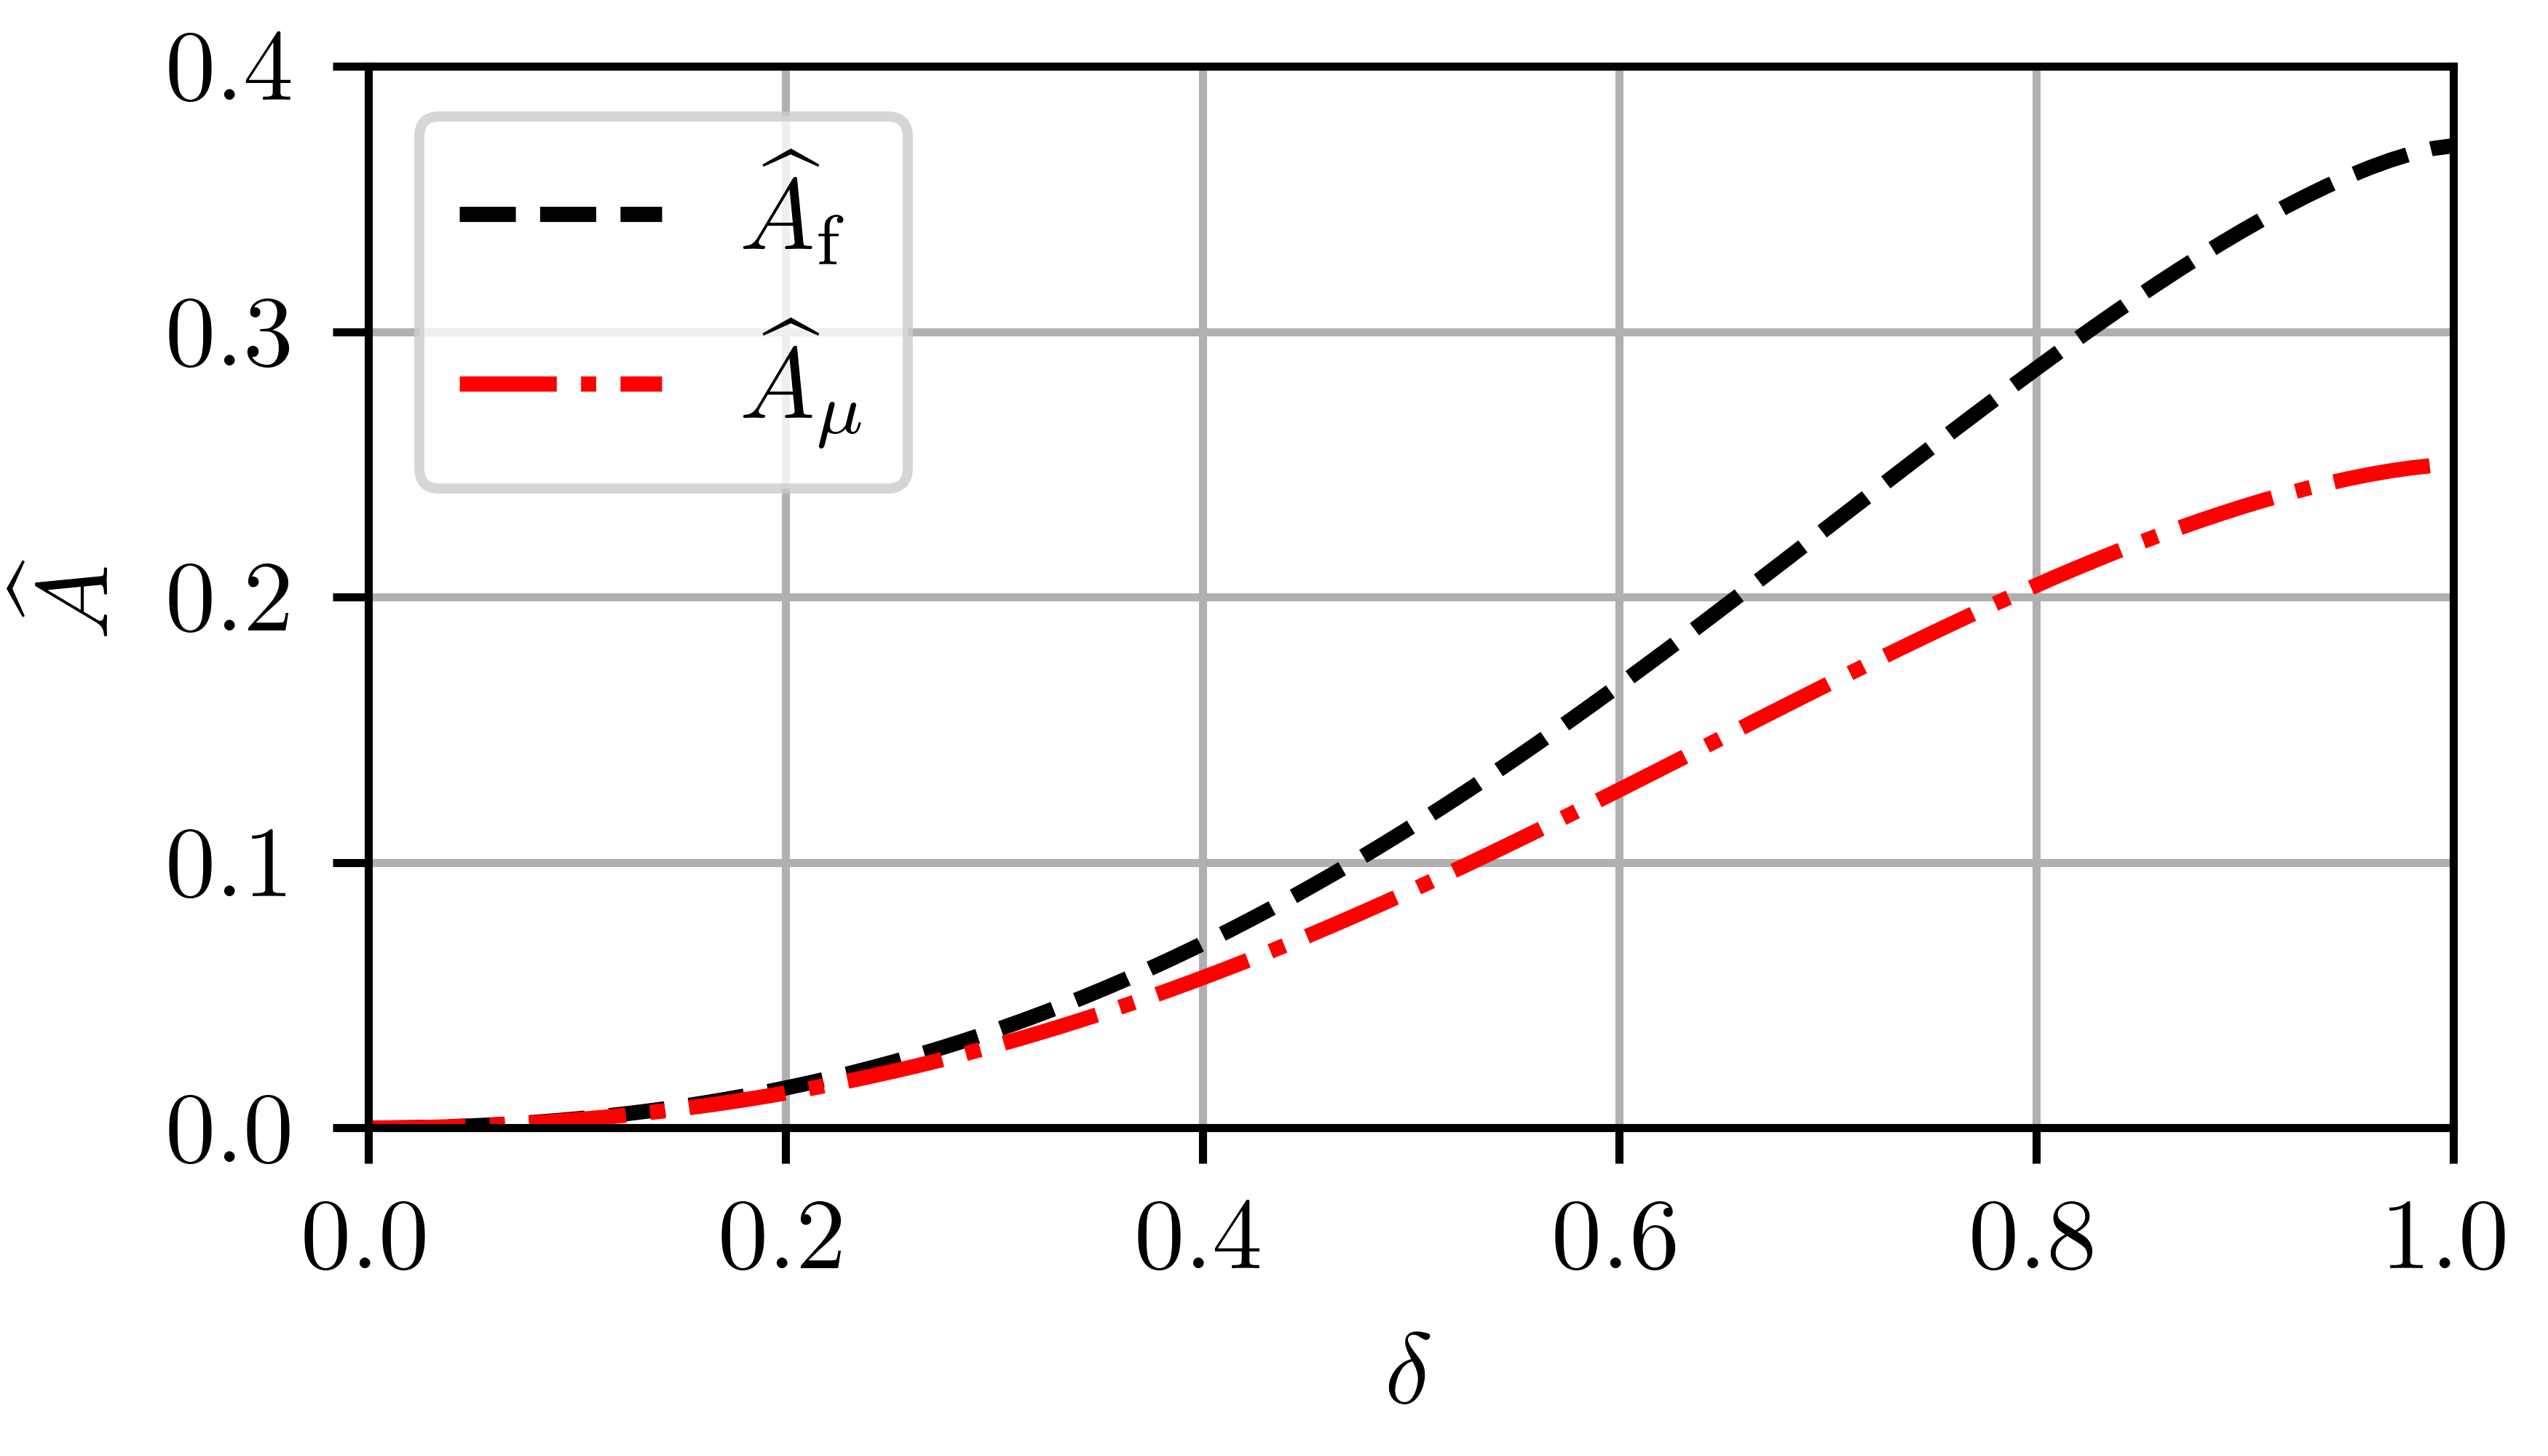
\includegraphics{3_chapters/0_introduction/img/AE.png}
    \caption{The \AE{} of the single waterbag distribution for both the case where there are no additional invariants, and $\mu$ is an invariant.}
    \label{fig: aes of the example}
\end{figure}
To gain some insight into the complex functional forms, let us consider two limiting cases. First, we Taylor expand around the smallness of $\delta$ to the third order, which results in $\widehat{A}_{\rm f}\approx \frac{5}{16} \delta^2 + \frac{5}{16} \delta^3$. Expanding the constrained case to the third order in $\delta$ also results in $\widehat{A}_\mu \approx \frac{5}{16} \delta^2 - \frac{1}{12}\delta^{5/2} + \frac{5}{16} \delta^3 $. We thus find that, to leading order, the contributions are exactly the same, and it is the leading order correction where differences in the behaviour of the \AE{} are found. The other limiting case is $\delta=1$ for which one finds $\widehat{A}_{\rm f}=1-2^{-2/3}$, and $\widehat{A}_\mu=1/4$. Therefore, we see that the \AE{} in the unconstrained case is, perhaps unsurprisingly, higher than that of the constrained case. Finally, a graph showing the full behaviour of the \AE{}s is given in Fig. \ref{fig: aes of the example}. In this Fig. we see that increasing the gradient (parameterised by $\delta$) increases the amount of available energy, given formal weight to the mantra that gradients supply free energy. \par

Let us now take a step back and investigate what we have learnt from the above example. In all cases, we have seen that we were able to derive the ground state by means of Eq. \eqref{eq: integral for ground state} or its equivalent form differential form \eqref{eq:integro-diff for ground state}.  This ground state was typically a state in which gradients are flattened as much as is possible under the given constraints. Finally, we have seen that the calculation of the ground state and its associated energy is typically the most involved step in the calculation of \AE{}.\footnote{We note that, under certain conditions, one may short-circuit these calculations by assuming that the initial distribution function is close to a ground state. An explicit expression of \AE{} may then be derived, without the need to calculate the ground state explicitly, and this work is currently in preparation with Helander. However, one of these conditions is broken in the case of trapped electrons \AE{} and results in flawed expressions, and as such we present the full calculation here.} These observations will remain true as we investigate more intricate cases, in which closed form analytical expressions of \AE{} are not available. If we impose that both $\mu$ and $\mathcal{J}$ be conserved, we will encounter exactly one such case.

\section{The \AE{} to be investigated}
As indicated in previous sections, this thesis focusses on the \AE{} of trapped electrons, in which Liouville's theorem, invariance of $\mu$, and constancy of $\mathcal{J}$ are enforced. This is not the first investigation of such a scenario, as specialised cases were already investigated by \citet{helander2017available,helander2020available}. In these papers, Helander investigates (among other things) under what conditions the \AE{} of trapped electrons vanishes and subsequently calculated the \AE{} in the specialised case of omnigenous systems. Focussing on the former (as the latter will be generalised further in the thesis), it was found that \AE{} vanishes if two conditions are met. First, the device needs to be exactly omnigenous, meaning that trapped particles do not drift radially outward, or in terms of Eq. \eqref{eq: dJdalpha} one needs $\partial_\alpha \mathcal{J} = 0$. Second, the bounce-averaged binormal drift (encapsulated by $\omega_\alpha$ as in Eq. \eqref{eq: omega_alpha}) needs to be faster than the drift wave. For a density gradient-driven drift wave, such conditions are met in maximum-$\mathcal{J}$ devices, further highlighting their stabilising properties. \par 

The remarkable feature of this conclusion (which can be derived by relatively simple means) is that it reproduces exactly the linear gyrokinetic instability thresholds which were derived by \citet{proll2012resilience} in 2012, showing that it is also a nonlinear threshold. This makes it an especially promising candidate for application to turbulence, as it coincides with known gyrokinetic results. The \AE{} may then be interpreted as a distance measure from the instability thresholds, quantifying how unstable a system is. \par 

This is not to say that the results cannot be generalised further, to account for ions, passing electrons, or even more exotic scenarios. An attempt at such a generalisation was made in \cite{helander2020available}, where ion species and passing electrons were accounted for as well, which in turn were coupled via quasineutrality. Let us note, though, that the result of such a calculation is {\it highly} dependent on the chosen invariants, and one may arrive at different conclusions by making different choices. One other such choice shall be considered at the end of the thesis as well for passing electrons, with implications on transport. 

% *************************************************************
%%%% first part}
\cleardoublepage
\part{Publications}\label{part: publications}
%!TEX root = ../../thesis.tex
\chapter[Bounce-averaged drifts]{Bounce-averaged drifts}
\label{chap: BAD}
\begin{figure}
    \centering
    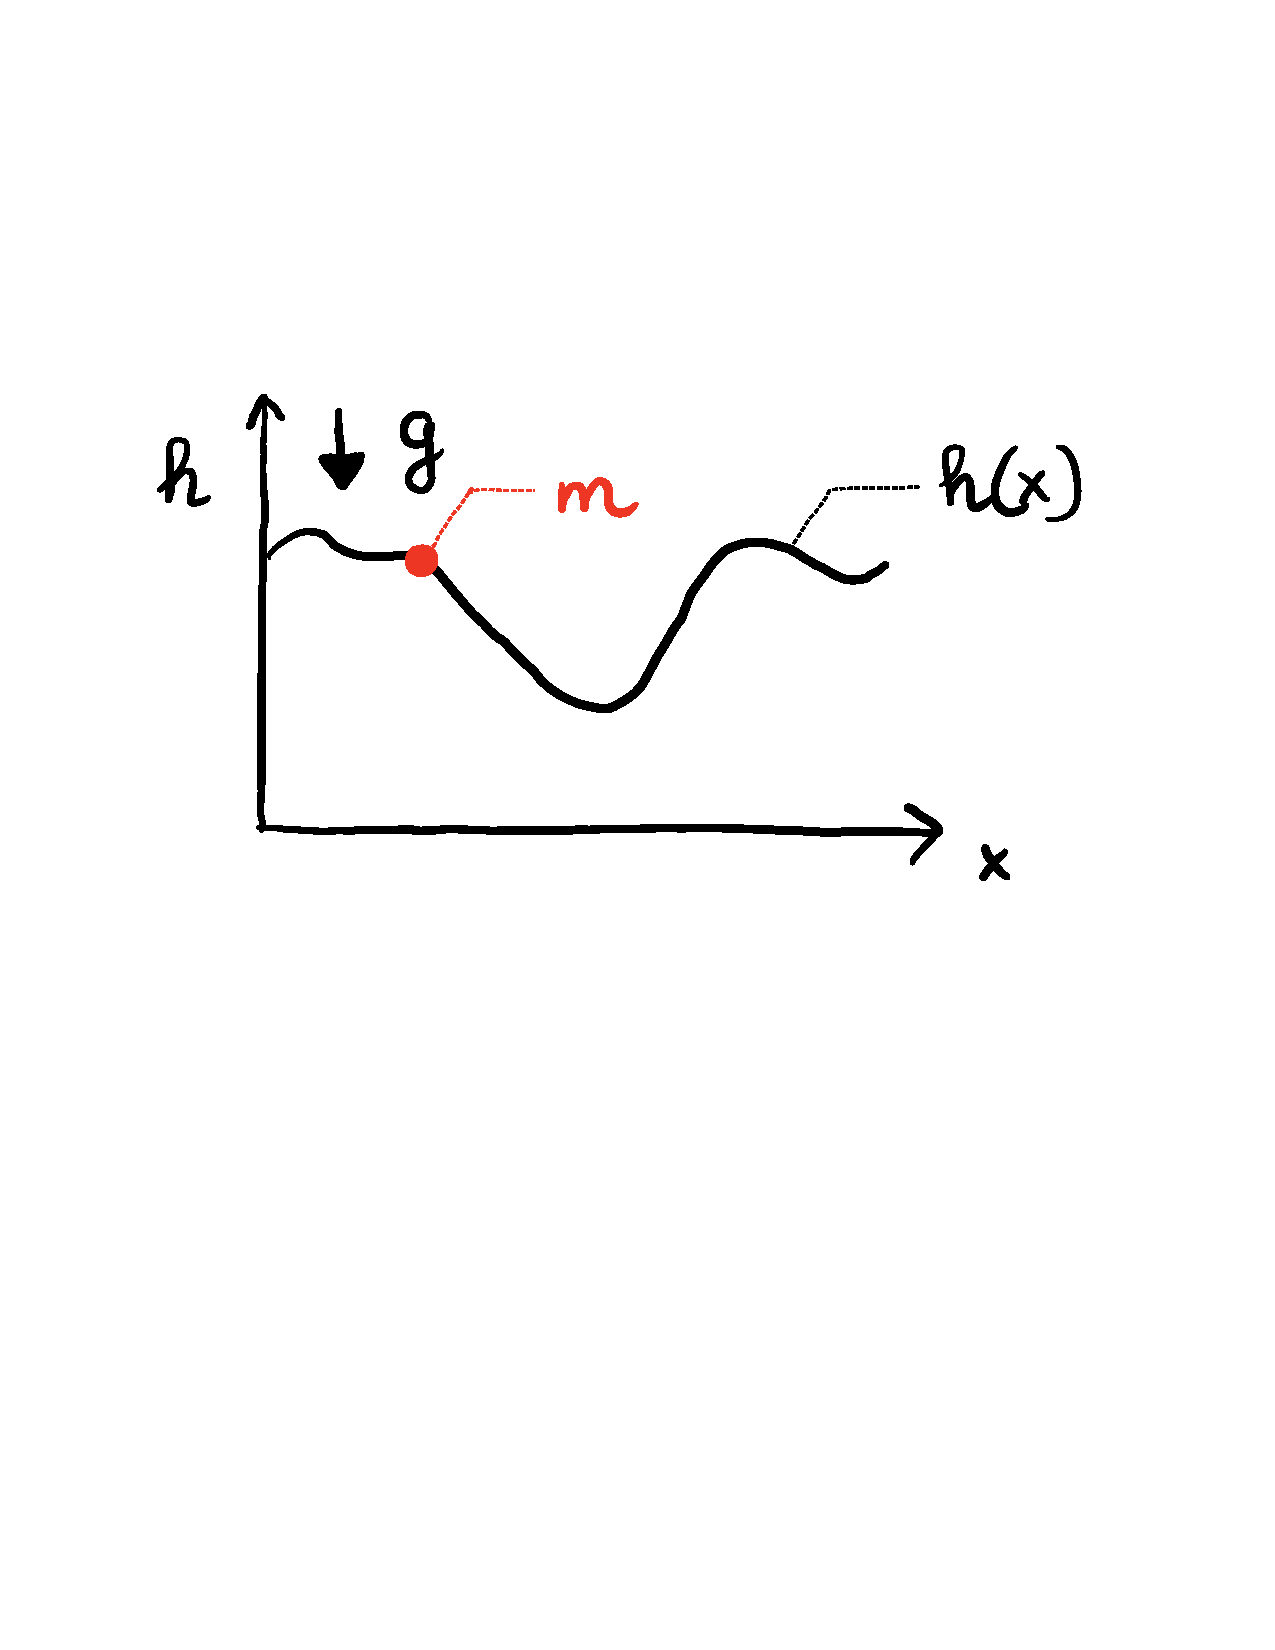
\includegraphics[width=0.5\textwidth]{3_chapters/1_papers/BAD/figures/bead-on-a-wire.pdf}
    \caption{A bead of mass $m$ in red, on a stiff wire prescribed by $h(x)$ in black, in a gravitational field with acceleration $g$.}
    \label{fig:bead on a wire}
\end{figure}
In the calculation of the \AE{} of trapped electrons, one requires accurate methods to calculate the bounce averaged drift a trapped particle experiences. Such a bounce-average is the time-average of some quantity which a trapped particle experiences, which may be thought of analogously to a bead on a stiff wire. This may be seen as follows: the total energy may be written as
\begin{equation}
    E = \mu B + \frac{1}{2}mv_\parallel^2 \implies v_\parallel = \pm \sqrt{\frac{2}{m}} \sqrt{E - \mu B}.
\end{equation}
Let us compare this quantity against the total energy of a bead on a wire in a gravitational field of constant acceleration, of which a sketch is given in Fig. \ref{fig:bead on a wire}. Here the total energy is given by
\begin{equation}
    E = mg h(x) + \frac{1}{2}mv^2 \implies v = \pm \sqrt{\frac{2}{m}} \sqrt{E - mgh(x)}.
\end{equation}
The equivalence is now obvious: the perpendicular energy $\mu B$ may be interpreted as a potential $mgh$. The bounce average of any quantity for the bead on a wire, which we denote by means of angular brackets, may now simply be thought of as
\begin{equation}
    \langle \dots \rangle \equiv \frac{ \int_{\rm bounce} \dots \mathrm{d} t }{ \int_{\rm bounce} \mathrm{d} t } = \frac{ \int_{\rm bounce} \dots \frac{\mathrm{d} \ell}{\sqrt{E - mgh}} }{ \int_{\rm bounce} \frac{\mathrm{d} \ell}{\sqrt{E - mgh}} },
    \label{eq: bounce average analogy}
\end{equation}
where the region of integration is one periodic motion of the point mass on the wire, and we have used the fact that $v = \mathrm{d}\ell/\mathrm{d}t$ with $\mathrm{d}\ell$ being the distance travelled by the point mass $m$ in time $\mathrm{d} t$. \par 
Though constructed by means of an analogy, Eq. \eqref{eq: bounce average analogy} may be used to readily find various properties emblematic of bounce-averages. Firstly, regions where the point mass is reflected (which will be referred to as bounce-points) have $v=0$, and the integrand becomes singular. Resolving this singular behaviour accurately is not a trivial task, and in the proceeding publication we put much emphasis on executing such integrals correctly numerically by including benchmark cases. Furthermore, if the bounce point approaches a local maximum, the point mass will spent all of its time near the local maximum and the time-average hence only cares about values near the local maximum. Again, if not this property is not handled properly, one may find erroneous bounce averages. By focusing on resolving such bounce-averaging integrals correctly the computational cost and accuracy of such calculations is greatly improved, which in turn will aid in the \AE{} calculations. Let us note in passing that this exercise in numerical rigour has found use outside of the current thesis as well, currently being used in works of P. Costello and E. Rodr\'iguez. Without further ado, the publication shall now be presented in unaltered shape.
\vfill \newpage


%!TEX root = ../../thesis.tex
\chapter[Available energy of trapped electrons]{Available energy of trapped electrons}
\label{chap: AE-TE}
With our understanding of the bounce-averaged drift cemented, we now shift our focus to the \AE{} of trapped electrons. Let us note that this publication has been published in two parts. Firstly, a highly condensed version of the results presented was published as a {\it Physical Review Letter} for a general physics audience \cite{mackenbach2022available}. In a later publication, we included additional findings in the research and gave more details of the derivation, and this publication is what we include in the thesis. The publication focusses on the \AE{} of trapped electrons, as eluded to before, where the result of \cite{helander2020available} will be generalised to account for radially drifting trapped particles. The generalised expression of the \AE{} of trapped electrons allows us to compare it with nonlinear gyrokinetics in general magnetic geometries. Before the research, it was unknown whether \AE{} of trapped electrons can be used to predict turbulent transport, and in the following research we find predictive capabilities. This finding is encouraging, as it implies that \AE{} can be used as a measure of turbulent transport in general systems, making it useful in, e.g., optimisation loops. \vfill \newpage

\section*{The available energy of trapped electrons: a nonlinear measure for turbulent transport}
\small{R.J.J. Mackenbach$^{1,2}$, J.H.E. Proll$^{1,2}$, R. Wakelkamp$^{3}$ P. Helander$^{2}$} \\
\small{$^1$ Eindhoven University of Technology, 5612 AZ, Eindhoven, Netherlands} \\
\small{$^2$ Max Planck Institute for Plasma Physics, 17491 Greifswald, Germany} \\
\small{$^3$ Utrecht University, 3584 CS Utrecht, The Netherlands}


\chapterabstract{A collisionless plasma possesses a certain amount of ``available energy'', which is that part of the thermal energy that can be converted into kinetic energy of plasma motion and electromagnetic fluctuations. In this paper we present a calculation of the available energy carried by trapped electrons in a slender non-omnigenous flux tube of plasma. This quantity is compared with gyrokinetic simulations of the nonlinear saturated radial energy flux resulting from turbulence driven by collisionless trapped-electron modes in various stellarators and a tokamak. The numerical calculation of available energy is fast and shows a strong correlation with the turbulent energy fluxes found in the gyrokinetic simulations. Indeed, the energy flux is found to be proportional to the available energy to the power of approximately $3/2$, which is what one would expect from a simple argument. We furthermore investigate how available energy is distributed across different bounce wells, and it is found that deeply trapped electrons typically contribute most to the available energy. Finally, we investigate the dependence of available energy on gradient strength, and we find important differences between weakly and strongly driven regimes for stellarators and tokamaks.}

\section{Introduction} \label{sec:outline}
    One of the major challenges facing magnetically confined fusion plasmas is the degradation of energy confinement due to transport. This transport arises because the density and temperature vary across the plasma volume, giving rise to neoclassical transport as well as free energy which drives instabilities, turbulence, and transport. The dependence on the geometry of the magnetic field is well understood in the case of neoclassical transport, and stellarators can be designed in such a way as to minimize these losses \citep{Wolf2017MajorStellarator,Klinger2019OverviewOperation,Dinklage2018MagneticStellarator,beidler2021demonstration}. \par
    The main transport channel is then turbulent transport, which typically exceeds the neoclassical channel, see e.g. \citet{Bozhenkov2020High-performance7-X,beidler2021demonstration}. Accordingly, insights into the interplay between turbulence and geometry are desired so that one can understand, and perhaps minimize, the turbulent losses. However, due to the complex nonlinear nature of the problem, it has proved difficult to quantify the dependence of turbulence on geometry, though significant strides have been made in recent years \citep{Barnes2011CriticallyPlasmas,Proll2012ResilienceInstabilities,Proll2022TurbulenceGradient,Pueschel2016StellaratorModeling,Citrin2017TractableQuaLiKiz,Helander2013CollisionlessModes,Plunk2014CollisionlessMode}. 
    These methods, though not all of them, typically employ (quasi-)linear theory to estimate the turbulence properties for any given configuration. Such methods do not always capture important nonlinear effects and suffer, in particular, from uncertainties concerning the turbulent saturation amplitude. The most reliable option to assess nonlinear turbulent transport is to carry out nonlinear gyrokinetic simulations \citep{Beer1995FieldTurbulence,Garbet2010GyrokineticTransport}, but it is currently computationally expensive to do so, though significant improvements have been made \citep{Mandell2022GX:Design}. \par
    In a recent publication \citep{Mackenbach2022AvailableTransport}, it was shown that the so-called available energy (\AE{}) can provide a quantitative estimate of the turbulence driven by the trapped-electron mode \citep{Kadomtsev1967PlasmaGeometry,Dannert2005GyrokineticTurbulence}, and in the present paper we elaborate on the mathematical details of this calculation. 
    \par
    The \AE{} of a system is defined as the difference in energy between the ``initial'' distribution function $f_i$ (i.e. the distribution function at time $t=0$), and the so-called ground state $f_g$ \citep{Lorenz1955AvailableCirculation,Gardner1963BoundPlasma}. The latter is the distribution function which minimizes the energy, subject to constraints imposed by the Vlasov equation. We encapsulate the constraints that follow from Liouville's theorem in the following invariant
    \begin{equation}
    H[f(\boldsymbol{x},t),\phi] \equiv \int \Theta[f(\boldsymbol{x},t)-\phi] \mathrm{d} \boldsymbol{x},
    \label{eq:vlasov-invariant}
    \end{equation}
    where $\Theta[x]$ is the Heaviside function, $\phi$ is a scalar constant, and $\boldsymbol{x}$ are the phase-space coordinates, $(\boldsymbol{r},\boldsymbol{v})$. If the distribution function $f$ evolves according to the Vlasov equation or any other equation that conserves phase-space volume, one can show that $H[f,\phi]$ is conserved for every $\phi \in \mathbb{R}$ \citep{Helander2017AvailablePlasmas}. Furthermore, we define the energy of the distribution function as
    \begin{equation}
        E[f(\boldsymbol{x},t)] \equiv \int \epsilon (\boldsymbol{x}) f(\boldsymbol{x},t) \mathrm{d} \boldsymbol{x},
    \label{eq:energy-functional}
    \end{equation}
    where $\epsilon(\boldsymbol{x})$ is the energy of a particle (typically $mv^2/2$). With these definitions, the ground state can be denoted as the distribution function t minimizes the functional
    \begin{equation}
        W[f_g,\lambda] = E[f_g] + \int \lambda(\phi) \left( H[f_i,\phi] - H[f_g,\phi] \right) \mathrm{d}\phi
    \end{equation}
    where $\lambda(\phi)$ denotes a continuous set of Lagrange multipliers. \par
    If one evaluates the variation of $W$ with respect to $f_g$, and requires that the distribution function be a stationary point of the functional (that is $\delta W/\delta f_g=0$), one finds that a ground state must be a function of energy alone,
    \begin{equation}
        f_g = f_g(\epsilon).
        \label{eq:ground-state-dependencies}
    \end{equation}
    Furthermore, if one considers the second variation with respect to $f_g$ and demands that this quantity be positive definite (so that the ground state is a local minimum of the functional), one finds that the ground state must be a decreasing function of energy
    \begin{equation}
        \frac{\partial f_g}{\partial \epsilon} \leq 0.
        \label{eq:ground-state-energy-dependence}
    \end{equation}
    \par
    One can also impose the condition that a set of adiabatic invariants, denoted by $\boldsymbol{y}$, should be conserved (as in \cite{Helander2017AvailablePlasmas,Helander2020AvailablePlasmas}), thus adding more constraints than equations \eqref{eq:ground-state-dependencies} and \eqref{eq:ground-state-energy-dependence}. The ground states are then functions satisfying
    \begin{subequations}
    \begin{equation}
        f_g = f_g(\epsilon, \boldsymbol{y}),
    \end{equation}
    \begin{equation}
        \left( \frac{\partial f_g}{ \partial \epsilon } \right)_{\boldsymbol{y}}  \leq 0.
    \end{equation}
        \label{eq:ground-state-decrease-adiabatic}
    \end{subequations}
    \par 
    From these criteria it is possible to derive an integro-differential equation for the ground state. For instance, it has been shown that, if we choose the magnetic moment $\mu$ and the parallel invariant $\mathcal{J}$ as adiabatic invariants, the ground state $f_g(\epsilon,\mu,\mathcal{J})$ must obey the following integro-differential equation \citep{Helander2020AvailablePlasmas}
    \begin{equation}
    \begin{aligned}
        \left( \frac{ \partial f_g(w,\mu,\mathcal{J})}{\partial w} \right)_{\mu,\mathcal{J}} = - \frac{\iint \delta [w - \epsilon(\psi,\alpha,\mu,\mathcal{J})] \mathrm{d}\psi \mathrm{d}\alpha }{\iint \delta[f_i - f_g(w,\mu,\mathcal{J})] \mathrm{d}\psi \mathrm{d}\alpha }.
    \end{aligned}
    \label{eq:ground-state-eq}
    \end{equation}
    Here $w$ is a positive scalar which acts as a placeholder for the particle energy $\epsilon$, $\psi$ is the magnetic flux (i.e. the flux-surface label) and $\alpha$ is the Clebsch angle, which locally define the magnetic field as $\boldsymbol{B} = \nabla \psi \times \nabla \alpha $ \citep[see][ch.~5]{Dhaeseleer2012FluxTheory}. Equation \eqref{eq:ground-state-eq} is relevant for most kinds of gyrokinetic turbulence in tokamaks and stellarators, since $\mu$ and $\mathcal{J}$ are typically conserved quantities for trapped electrons in the case of microinstabilities and turbulence with wavelengths comparable to the ion gyroradius. 
    \par
    In the literature, most numerical simulations of such phenomena are performed in the geometry of a slender flux tube aligned with the magnetic field, and in this limit Eq.~(\ref{eq:ground-state-eq}) can be solved analytically. For the case of a vanishingly slender flux tube under the condition of omnigenity, i.e. that the second adiabatic invariant $\mathcal{J}$ is independent of the Clebsch angle $\alpha$ (i.e. $\partial \mathcal{J} / \partial \alpha = 0$), explicit expressions for the ground state and the \AE{} have been found \citep{Helander2020AvailablePlasmas}. This derivation shows that a Maxwellian distribution function can only be a ground state if the magnetic field is omnigenous and if the electron diamagnetic drift frequency $\omega_*^T$ does not exceed the bounce-averaged precession frequency $\omega_\alpha$,
    \begin{equation}
        \omega_*^T/\omega_\alpha \leq 1,
        \label{eq:stability-crit}
    \end{equation}
    for all types of trapped-electron orbits in the flux tube. Here the diamagnetic drift frequency is equal to
    \begin{equation}
        \omega_*^T = \frac{T}{q} \left[ \frac{\mathrm{d} \ln n}{\mathrm{d} \psi} + \frac{\mathrm{d} \ln T}{\mathrm{d} \psi} \left( \frac{\epsilon}{T} - \frac{3}{2} \right) \right],
    \end{equation}
    where $T$ is the temperature, $n$ is the number density, $\epsilon$ is the particle energy, and $q$ is the particle charge.
    The criteria of \eqref{eq:stability-crit} are met in quasi-isodynamic stellarators with the so-called maximum-$\mathcal{J}$ property, and it has been shown from the (linear) gyrokinetic equations that these devices are indeed resilient against conventional density-gradient-driven TEMs by \citep{Proll2012ResilienceInstabilities,Helander2013CollisionlessModes}. When these modes are stabilised, other, less virulent, instabilities become dominant instead \citep{Helander2015TheGeometry,Plunk2017CollisionlessMode,costello2023universal}.
    \par 
    In this paper we first extend the calculation of \AE{} to non-omnigenous flux-tubes, which is of relevance since most stellarators are, in fact, not omnigenous. We first show that such a calculation is most easily done in flux tubes which have an elliptical cross-section. This calculation is described in section \ref{sec:theory}, where we also discuss how the \AE{} can be computed numerically. In section \ref{sec:results} we compare the numerically calculated \AE{} in a tokamak and various stellarators with the turbulent energy flux computed by the gyrokinetic code \textsc{gene} \citep{Jenko2000ElectronTurbulence}. These results were recently published in abbreviated form \citep{Mackenbach2022AvailableTransport}, and here we provide full mathematical details. We furthermore investigate which types of trapped particles contribute most to \AE{}, and find that deeply trapped particles typically do so. We also establish that the dependence on the gradient strength is non-trivial and investigate this dependence in some depth. Finally, in section \ref{sec:conclusions}, we highlight our most important findings and discuss future directions for research. 
 
\section{The ground state and available energy in a flux-tube} \label{sec:theory}
\subsection{Allowable domains}
In the calculation of the ground state, we restrict our attention to a subregion of the plasma which has the shape of a slender flux tube aligned with the magnetic field, allowing us to approximate the distribution function by its first-order Taylor expansion in the directions perpendicular to the field. Only then does it seem possible to solve the integro-differential ground-state equation (\ref{eq:ground-state-eq}) in general. Somewhat surprisingly, it turns out that the calculation is only possible if the cross section of the flux tube is elliptical, as we shall now see. 

We first introduce the following re-scaled coordinates,
\begin{subeqnarray}
    x &&= (\psi - \psi_0)/\Delta \psi, \\
        y &&= (\alpha - \alpha_0)/\Delta \alpha.
        \label{eq:altered-coordinates}
\end{subeqnarray}
Here, $\psi_0$ and $\alpha_0$ are the flux-surface label and field-line label of the magnetic field line defining the centre of the flux tube, and $\Delta \psi$ and $\Delta \alpha$ define its scale lengths in the $\psi$- and $\alpha$-directions, respectively. In contrast to the situation in most gyrokinetic simulations, the cross section of the flux tube is not assumed to be rectangular. In these coordinates, we denote the first-order expansion of the distribution function $f$ for fixed values of $\mu$, $\mathcal{J}$, and $t$ by
\begin{equation}
        f(x,y,\mu,\mathcal{J},t) \equiv f_0 + f_{x} x + f_{y} y.
        \label{eq:expansion}
\end{equation}
For a given smooth distribution function, this representation should always be sufficiently accurate in the limit of small $\Delta \psi$ and $\Delta \alpha$ (i.e. for small enough $\psi - \psi_0$ and $\alpha - \alpha_0$ one can approximate $f \approx f_0 + (\psi - \psi_0) \partial_\psi f + (\alpha - \alpha_0) \partial_\alpha f$), but there is no guarantee that the ground state corresponding to such a function can be similarly approximated by its linear expansion. Indeed, this turns out to be true, in general, only if the domain $\Omega$ in the $(x,y)$-plane under consideration is elliptical. 
As already mentioned, phase-space volume conservation dictates that the following integral is independent of time for all values of $\phi$,
\begin{equation}
    \frac{\mathrm{d}}{\mathrm{d} t}\int_{\Omega} \Theta \left[ \phi - f(x,y,\mu,\mathcal{J},t) \right] \mathrm{d} x \mathrm{d} y = 0.
    \label{eq:vlasov-inv}
\end{equation}
In particular, this integral must be the same for the initial (given) distribution function and its corresponding ground state. We assume that both can be described by their linear approximations (\ref{eq:expansion}), whose gradients will, however, in general point in different directions (i.e. $\nabla_\perp f \propto \hat{\boldsymbol{x}} f_x +\hat{\boldsymbol{y}} f_y$ can take on any value, with the hatted quantities denoting unit vectors). We thus require that the gradient of the ground state may point in an arbitrary direction and derive a constraint on the shape of $\Omega$ from this condition.

It is useful to define a rotated coordinate system $(x,y)\mapsto(\tilde{x},\tilde{y})$, 
\begin{equation}
\begin{aligned}
\tilde{x} &= x \cos \vartheta + y \sin \vartheta + x_{\rm min}(\vartheta), \\
\tilde{y} &= - x \sin \vartheta + y \cos \vartheta + y_{\rm min}(\vartheta),
\end{aligned}
\end{equation}
such that $f$ assumes its smallest value, $f_{\rm min}$, at $\tilde x = 0$ and the gradient of $f$ points in the direction of $\tilde x$:
\begin{equation}
    f = f_\mathrm{min} + f_{\tilde{x}} \tilde{x}.
\end{equation}
In such a coordinate system the domain rotates as the function evolves, whilst fixing the minimal values of $x$ and $y$ to $\tilde{x}=\tilde{y}=0$, and this coordinate system will aid us in making statements about this domain shape. The initial state and the ground state thus correspond to two different values of $\vartheta$. The width of the domain $\Omega$ in the $\tilde x$-direction is denoted by $2D(\vartheta)$, so that the maximum value of $f$ becomes $f_\mathrm{max} = f_\mathrm{min} + 2 D f_{\tilde{x}}$, and the distribution function may be written as
\begin{equation}
    f = f_\mathrm{min} + \frac{\tilde{x}}{2D} \left( f_\mathrm{max} - f_\mathrm{min} \right),
\end{equation}
where we note that $f_\mathrm{min}$ and $f_\mathrm{max}$ depend only on $\mu$ and $\mathcal{J}$ and are thus independent of $\vartheta$. 

We now return to the problem at hand, codified by Eq. \eqref{eq:vlasov-inv}. The argument of the Heaviside function vanishes in the new coordinate system when
\begin{equation}
    \tilde{x}(\phi) = 2D \frac{\phi - f_\mathrm{min}}{f_\mathrm{max}-f_\mathrm{min}}.
        \label{eq:zero-of-heaviside}
\end{equation}
Let us now consider a value of $\phi$ very close to $f_\mathrm{min}$, i.e. $\phi = f_\mathrm{min} + |\epsilon|$ with $|\epsilon| \rightarrow 0^+$. Eq. \eqref{eq:zero-of-heaviside} now reduces to $\tilde{x}_\epsilon = 2D|\epsilon|/(f_\mathrm{max}-f_\mathrm{min})$. The integral in Eq.~(\ref{eq:vlasov-inv}) is equal to the area of the subdomain of $\Omega$ over which $f \le \phi$, i.e. the coloured region in Fig. \ref{fig:sketch-of-area}. In the limit $\tilde{x}_\epsilon \ll D$, the radius of curvature, $R$, of the domain boundary in the region $\tilde x < \tilde x_\epsilon$ is approximately constant (if the boundary is sufficiently smooth). Hence, we may approximate the integral by instead considering the area of a circular segment with the same radius of curvature $R$,
\begin{equation}
\begin{aligned}
    \mathcal{A} &= 2\int_0^{\tilde{x}_\epsilon} \sqrt{2R\tilde{x}  - \tilde{x}^2} \: \mathrm{d} \tilde{x}  \\
    &\approx 2 \int_0^{\tilde{x}_\epsilon} \sqrt{2 R\tilde{x} } \: \mathrm{d} \tilde{x} = \frac{4}{3} \sqrt{2 R \tilde{x}_\epsilon^3},
\end{aligned}
\label{eq:circular-segment}
\end{equation}
\begin{figure}
    \centering
    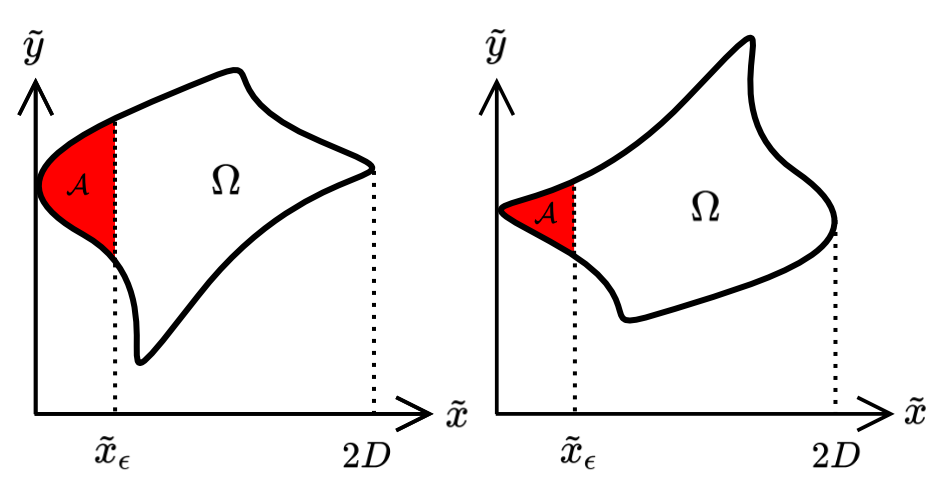
\includegraphics[width=1.0\textwidth]{3_chapters/1_papers/AE-TE/figures/boundary-setup.png}
    \caption{A sketch of the area, coloured red, as a subset of the entire domain $\Omega$. Done at two different times, so that the orientation of the domain $\Omega$ is different.}
    \label{fig:sketch-of-area}
\end{figure}
where we have used the equation for a circle $\tilde{y}^2 = R^2 - (\tilde{x} - R)^2 $. The next step is to realise that, as the distribution function evolves, its gradient may point in any direction in the $(x,y)$-plane, so that the angle $\vartheta$ may assume any value. A sketch of the domain at a different orientation is also given in Fig. \ref{fig:sketch-of-area}. Both $D$ and $R$ depend on $\vartheta$, but they are not independent. Indeed, from Eq. \eqref{eq:vlasov-inv}  we have
\begin{equation}
    R(\vartheta)D(\vartheta)^3 = C_\mathcal{A} = \mathrm{constant},
\end{equation}
where we have used the equation for the area found in \eqref{eq:circular-segment}. In particular, the radius of curvature is the same at the two extremal locations $\tilde{x}=0$ and $\tilde{x}=2D$, since a rotation of $\pi$ leaves $D$ unchanged. Moreover, on purely geometrical grounds there is a relation between the second derivative of the domain width and the curvature, as shown in Appendix \ref{app:diff-for-domain},
\begin{equation}
    \frac{\mathrm{d}^2 D}{\mathrm{d} \vartheta^2} = R - D.
\end{equation}
Using the constancy of $RD^3$, we find that
\begin{equation}
    \frac{\mathrm{d}^2 D}{\mathrm{d} \vartheta^2} + D = \frac{C_\mathcal{A}}{D^3} \implies \frac{\mathrm{d}}{\mathrm{d} \vartheta} \left[\left(\frac{\mathrm{d} D}{\mathrm{d} \vartheta}\right)^2 + D^2 + \frac{C_\mathcal{A}}{D^2} \right]=0.
\end{equation}
As shown in Appendix \ref{app:diff-for-domain}, this differential equation has the general solution
\begin{equation}
    D(\vartheta) = (C^2-C_\mathcal{A})^{1/4}\sqrt{C + \cos 2 \vartheta},
\end{equation}
implying that the radius of curvature becomes
\begin{equation}
    R(\vartheta) = \frac{C_\mathcal{A}}{(C^2-C_\mathcal{A})^{3/4}(C + \cos 2 \vartheta)^{3/2}}.
    \label{eq:radius-of-curvature-main}
\end{equation}
The radius of curvature for an ellipse is of the exact same form as Eq. \eqref{eq:radius-of-curvature-main} (as shown in the Appendix \ref{app:diff-for-domain}), implying that $\Omega$ must be elliptical. We have thus found that the only domain shape in which Liouville's theorem can generally be satisfied is a slanted ellipse, if the distribution function is to be approximated by its first-order Taylor expansion in the coordinates perpendicular to the magnetic field.

\subsection{The ground state and the available energy}
As shown in the previous section the domain has to be a slanted ellipse, and here we shall derive what the ground state and \AE{} is in such a system. To this end, let us first realize that it is sufficient to calculate the \AE{} in an {\it unslanted} ellipse, which in the coordinates $x$ and $y$ of the previous section has the equation
\begin{equation}
    \frac{x^2}{a^2} + \frac{y^2}{b^2} = 1,
    \label{eq: circle equation}
\end{equation}
with $a \leq b$. We may then apply a rotation-operator, to find the result of any slanted ellipse. Let us start, then, by considering equation \eqref{eq:ground-state-eq} and one must evaluate integrals of the form
\begin{equation}
    I[h] = \int_\Omega \delta[h] \mathrm{d}\psi \mathrm{d}\alpha,
    \label{eq:dirac-delta}
\end{equation}
where $h(\psi,\alpha)$ is an arbitrary smooth function that vanishes in the centre of the domain, $h(0,0)=0$. This condition has to do with the fact that a constant Maxwellian is the ground state corresponding to an initial condition without gradients. As such, to lowest order the difference between the Maxwellian and the ground state should vanish, implying that $h(0,0)=0$ for the functions appearing in \eqref{eq:ground-state-eq}. Since we take the flux tube to be slender, we approximate the function $h$ as
\begin{equation}
    h(\psi,\alpha) \approx x \Delta \psi \partial_\psi h + y \Delta \alpha \partial_\alpha h.
\end{equation} 
We next define the vector $\boldsymbol{p} = \left( x, y \right)$, so that one can write the linear expansion of $h$ as
\begin{equation}
    h \approx \boldsymbol{p} \cdot \boldsymbol{n} |\partial_{\boldsymbol{p}} h|,
\end{equation}
where we have defined $\boldsymbol{n} \equiv \partial_{\boldsymbol{p}} h/ |\partial_{\boldsymbol{p}} h| $, and derivatives of $h$ are evaluated at the centre of the flux tube. Equation \eqref{eq:dirac-delta} then becomes,
\begin{equation}
    I[h] = \frac{\Delta \psi \Delta \alpha }{|\partial_{\boldsymbol{p}} h|} \int_\Omega \delta[\boldsymbol{p} \cdot \boldsymbol{n}] \mathrm{d}x \mathrm{d}y.
\end{equation}
The integral measures the length of the line where $h=0$ in the domain, which may be found as follows. We realise that this line satisfies the equation
\begin{equation}
    y = -\frac{h_x}{h_y} x,
\end{equation}
where we have used the notation $h_x \equiv \partial_x h$. We may now find its intersection with Eq. \eqref{eq: circle equation}, and one may readily verify that the intersection satisfies the equation
\begin{equation}
    x^2 + y^2 = (ab)^2 \frac{(h_x)^2+( h_y)^2}{(a h_x)^2+(b h_y)^2},
\end{equation}
with which the integral becomes
\begin{equation}
\begin{aligned}
    I[h] &= \frac{\Delta \psi \Delta \alpha }{|\partial_{\boldsymbol{p}} h|}  2ab\sqrt{\frac{h_x^2 + h_y^2}{(a h_x)^2+(b h_y)^2}} \\
    &= \Delta \psi \Delta \alpha \frac{ 2 ab }{\sqrt{(ah_x)^2+(bh_y)^2}},
    \label{eq: unslanted ellipse ground state}
\end{aligned}
\end{equation}
Our final step is to rotate the domain, which is equivalent to rotating the vector $\partial_{\boldsymbol{p}} h$, for which one can use the rotation mapping
\begin{subeqnarray}
    h_x &&\mapsto h_x \cos \vartheta - h_y \sin \vartheta, \\
    h_y &&\mapsto h_x \sin \vartheta + h_y \cos \vartheta,
        \label{eq: rotation of h}
\end{subeqnarray}
where $\vartheta$ measures the angle of rotation. Combining results of Eqs. \eqref{eq: unslanted ellipse ground state} and \eqref{eq: rotation of h}, we find
\begin{equation}
\begin{aligned}
    I[h] &= \frac{\Delta \psi \Delta \alpha}{ b \sqrt{  h_x^2 + h_y^2 - \mathcal{E}_\vartheta^2 } } \\
    \mathcal{E}_\vartheta(h_x,h_y) &\equiv e \left( h_x \cos \vartheta - h_y \sin \vartheta  \right)
\end{aligned}
\end{equation}
where the eccentricity $e \in [0,1) $ is defined as $e^2 \equiv 1 - a^2/b^2$. We are now in a position to evaluate the ground state; first choose the initial distribution function to be a Maxwellian (as usually done in gyrokinetic simulations), 
\begin{equation}
    f_M = n(\psi) \left( \frac{m}{2 \upi T(\psi)} \right)^{3/2} e^{-\epsilon/T(\psi)}.
\end{equation}
Here, $n(\psi)$ is the number density, $m$ is the electron mass, and $T(\psi)$ is the electron temperature. The spatial derivatives of the distribution and energy function can be related to the bounce-averaged precession frequencies of the electron orbits (as shown in Appendix \ref{sec:appendix-bounce-freq}),
\begin{subequations}
\begin{equation}
    \left(\frac{\partial \epsilon}{\partial \psi}\right)_{\mu,\mathcal{J},\alpha} = + q \omega_\alpha,
\end{equation}
\begin{equation}
    \left(\frac{\partial \epsilon}{\partial \alpha}\right)_{\mu,\mathcal{J},\psi} = - q \omega_\psi,
\end{equation} 
\begin{equation}
    \left(\frac{\partial f_{M}}{\partial \psi}\right)_{\mu,\mathcal{J},\alpha} = + q \frac{f_{M,0}}{T_0} \left( \omega_*^T - \omega_\alpha \right),
\end{equation}
\begin{equation}
    \left(\frac{\partial f_{M}}{\partial \alpha}\right)_{\mu,\mathcal{J},\psi} = + q \frac{f_{M,0}}{T_0} \omega_\psi,
\end{equation}
\end{subequations}
\label{eq:precession-frequencies}
\end{subeqnarray}
Here, quantities with the subscript zero are quantities that are evaluated at the centre of the flux-tube, $q$ is the electron charge, $\omega_\psi$ is the drift (precession) frequency in the $\psi$ direction, $\omega_\alpha$ is the corresponding frequency in the $\alpha$ direction, and $\omega_*^T$ is the electron diamagnetic frequency. With these expressions, the numerator in the equation (\ref{eq:ground-state-eq}) for the ground state becomes
 \begin{equation}
    \begin{aligned}
    \iint \delta \left[ w - \epsilon_0(\mu,\mathcal{J}) - q \omega_\alpha \psi + q \omega_\psi \alpha \right] \mathrm{d}\psi \mathrm{d}\alpha 
    = \\
    \frac{\Delta \psi \Delta \alpha }{|qb| \sqrt{(\omega_\alpha \Delta \psi )^2 + (\omega_\psi \Delta \alpha )^2 - (\mathcal{E}_\vartheta)^2 }},
    \end{aligned}
\end{equation} 
The denominater of Eq. \eqref{eq:ground-state-eq} can be calculated in a similar manner. We conclude that the ground-state distribution function has the following derivative,
\begin{equation}
    \begin{aligned}
        &\left( \frac{ \partial f_g(w,\mu,\mathcal{J})}{\partial w} \right)_{\mu,\mathcal{J}} = - \frac{f_{M,0}}{T_0} F, \\
        &F \equiv \frac{\sqrt{(\omega_*^T - \omega_\alpha)^2 (\Delta \psi)^2 + \omega_\psi^2 (\Delta \alpha)^2 - \mathcal{E}_\vartheta ( \Delta \psi [\omega_*^T-\omega_\alpha], \Delta \alpha \omega_\psi )^2 }}{\sqrt{\omega_\alpha^2 (\Delta \psi)^2 + \omega_\psi^2 (\Delta \alpha)^2- \mathcal{E}_\vartheta ( \Delta \psi \omega_\alpha, -\Delta \alpha \omega_\psi )^2} }.
    \end{aligned}
\end{equation}
Since the right-hand side is negative, the solution decreases with increasing energy, which is a requirement for any ground state. In the limit of omnigenity (thus $\omega_\psi = 0$) one may verify that the terms involving $\mathcal{E}_\vartheta$ cancel, and one retrieves the expression previously found by \citet{Helander2020AvailablePlasmas}. 
To evaluate the \AE{}, we must find the difference in energy between the initial distribution function and the ground state,
\begin{equation}
    A = \int \epsilon \left( f_i - f_g \right) \sqrt{g} \mathrm{d}\psi \mathrm{d}\alpha \mathrm{d}\mu \mathrm{d}\mathcal{J}.
\end{equation}
Here, $\sqrt{g}$ denotes the phase-space Jacobian, which reduces to $\sqrt{g}= 4 \upi / m^2$ \citep{Helander2017AvailablePlasmas}. Moreover, $f_i$ and $f_g$ can be approximated by their Taylor expansions, 
\begin{equation}
    \begin{aligned}
        f_g\left[ \epsilon(\psi,\alpha,\mu,\mathcal{J}),\mu,\mathcal{J} \right] 
        = f_{i,0} +  \left( \frac{\partial \epsilon}{\partial \psi} \psi + \frac{\partial \epsilon}{\partial \alpha} \alpha \right) \left. \frac{ \partial f_g(w,\mu,\mathcal{J})}{\partial w} \right|_{w = \epsilon_0}
        + \cdots.
    \end{aligned}
\end{equation} 
It is useful to realize that the total number of particles within the domain for each pair of $\mu$ and $\mathcal{J}$ is conserved, giving
\begin{equation}
    \iint \left( f_i - f_g \right) \mathrm{d}\psi \mathrm{d}\alpha = 0,
\end{equation}
which in turn implies that the \AE{} can be calculated, to leading order, as
\begin{equation}
     A = \frac{4 \upi \Delta \psi \Delta \alpha}{m^2} \int \left( \Delta \psi^2 \frac{\partial \epsilon}{\partial \psi} \frac{\partial (f_i - f_g)}{\partial \psi} x^2 + \Delta \alpha^2 \frac{\partial \epsilon}{\partial \alpha} \frac{\partial (f_i - f_g)}{\partial \alpha} y^2 \right) \mathrm{d}x \mathrm{d}y \mathrm{d}\mu \mathrm{d}\mathcal{J}.
\end{equation}
The integration across $x$ and $y$ is readily carried out by rotating the function $x^2$ or $y^2$ by some angle, and integrating this function over the domain whose boundary is given in Eq. \eqref{eq: circle equation}. This may be readily calculated as
\begin{subeqnarray}
    \int_{\rm ellipse} (x \cos \vartheta - y \sin \vartheta )^2 &= \frac{\upi a^2b^2}{4} \left( \cos^2 \vartheta \sqrt{1-e^2} + \frac{\sin^2 \vartheta}{\sqrt{1 - e^2}} \right) &\equiv \frac{\upi a^2 b^2}{4} \hat{\mathcal{E}}_{\vartheta}^2, \\
    \int_{\rm ellipse} (y \cos \vartheta + x \sin \vartheta )^2 &= \frac{\upi a^2b^2}{4} \left( \sin^2 \vartheta \sqrt{1-e^2} + \frac{\cos^2 \vartheta}{\sqrt{1 - e^2}} \right) &\equiv \frac{\upi a^2 b^2}{4} \check{\mathcal{E}}_{\vartheta}^2.
\end{subeqnarray}
Our final step is to impose that this area of the ellipse is the same area as the unit circle ($a b = 1$), which may be achieved by an appropriate choice of $\Delta \psi$ and/or $\Delta \alpha$. We thus have
\begin{equation}
\begin{aligned}
    A = \upi^2 \left( \frac{ q \Delta \psi \Delta \alpha }{m}\right)^2 & \iint \frac{f_{M,0}}{T_0} \times   \\ 
    & \left[ \hat{\mathcal{E}}_{\vartheta}^2 \omega_\alpha^2 \left( \frac{\omega_*^T}{\omega_\alpha} - 1 +  F \right) \frac{\Delta \psi}{\Delta \alpha} +  \check{\mathcal{E}}_{\vartheta}^2\omega_\psi^2 \left( -1 + F \right) \frac{\Delta \alpha}{\Delta \psi} \right] \mathrm{d}\mu \mathrm{d}\mathcal{J} .
\end{aligned}
\end{equation}
Again, in the limit $\omega_\psi  \rightarrow 0$, the \AE{} reduces to the previously found expression \citep{Helander2020AvailablePlasmas}.\footnote{The result is nearly identical, up to the factor $\hat{\mathcal{E}}_\vartheta^2$. This factor may, however, be absorbed into $\Delta \psi$, resulting in the same equation as \citet{Helander2020AvailablePlasmas}.} The above equation is the central result of this paper, and may be interpreted as the most general result of the local available energy of trapped particles. To simplify further steps of the calculation, we shall specialise to the case in which the cross-section is circular in $(x,y)$, which implies $e = 0$. Note that this does not imply that the cross-section is also circular in $(\psi,\alpha)$-space: in these coordinates it is still an ellipse whose semi-major and semi-minor axes lie on lines of constant $\psi$ and $\alpha$. This furthermore has as the consequence that the various functions dependent on the angle of rotation and eccentricity simplify to $\mathcal{E}_\vartheta^2 = 0$,  $\hat{\mathcal{E}}_{\vartheta}^2=\check{\mathcal{E}}_{\vartheta}^2 = 1$, simplifying the calculations significantly. If one were to relax this condition it is useful to realise that the leading order correction in smallness of eccentricity is of order $\mathcal{O}(e^2)$, and the results may be trusted for small deviations.

% As shown in the previous section the domain has to be a slanted ellipse, and here we will rescale the length and width of the ellipse to be of length $x_\mathrm{max}-x_\mathrm{min} = y_\mathrm{max} - y_\mathrm{min} = 2$. This puts strict conditions on the shape the ellipse may take, as can be seen as follows. Let us start with the following parametric equation for the boundary of the ellipse in the $(x,y)$-plane,
% \begin{subeqnarray}
%     x &&= R_x \cos t \cos \varphi - R_y \sin t \sin \varphi, \\
%     y &&= R_x \cos t \sin \varphi + R_y \sin t \cos \varphi.
%         \label{eq:altered-coordinates}
% \end{subeqnarray}
% Here $t\in[0,2\pi)$ parameterises the boundary of the ellipse, $\varphi$ is the angle by which the ellipse is rotated, and $R_x$ and $R_y$ are the half widths of the ellipse in the $x$ and $y$ directions respectively if $\varphi = 0$. Since the total width $x_\mathrm{max}-x_\mathrm{min} = y_\mathrm{max} - y_\mathrm{min} = 2$, one can show that $\varphi = \pi/4$ and $R_y = \sqrt{2 - R_x^2}$ (and hence $R_x \in (0,\sqrt{2})$). A clarifying sketch of the ellipse as a function of $R_x$ is given in Fig. \ref{fig:parameterisation-Rx}. To find the ground state, as given in equation \eqref{eq:ground-state-eq}, we must evaluate integrals of the form
% \begin{equation}
%     I[h] = \int_\Omega \delta[h] \mathrm{d}\psi \mathrm{d}\alpha,
%     \label{eq:dirac-delta}
% \end{equation}
% where $h(\psi,\alpha)$ is an arbitrary smooth function that vanishes in the centre of the domain, $h(0,0)=0$. This condition has to do with the fact that a constant Maxwellian is the ground state corresponding to an initial condition without gradients. As such, to lowest order the difference between the Maxwellian and the ground state should vanish, implying that $h(0,0)=0$ for the functions appearing in \eqref{eq:ground-state-eq}. Since we take the flux tube to be slender, we approximate the function $h$ as
% \begin{figure}
%     \centering
%     \includegraphics[width=0.8\textwidth]{figures/ellipses.png}
%     \caption{Ellipses with $\varphi=\pi/4$ and $R_y = \sqrt{2-R_x^2}$ in the $(x,y)$-plane for various values of $R_x$. It can be seen that at $R_x=1$ the shape simplifies to a circle.}
%     \label{fig:parameterisation-Rx}
% \end{figure}
% \begin{equation}
%     h(\psi,\alpha) \approx x \Delta \psi \partial_\psi h + y \Delta \alpha \partial_\alpha h.
% \end{equation} 
% We next define the vector $\boldsymbol{p} = \left( x, y \right)$, so that one can write the linear expansion of $h$ as
% \begin{equation}
%     h \approx \boldsymbol{p} \cdot \boldsymbol{n} |\partial_{\boldsymbol{p}} h|,
% \end{equation}
% where we have defined $\boldsymbol{n} \equiv \partial_{\boldsymbol{p}} h/ |\partial_{\boldsymbol{p}} h| $, and derivatives of $h$ are evaluated at the centre of the flux tube. Equation \eqref{eq:dirac-delta} then becomes,
% \begin{equation}
%     I[h] = \frac{\Delta \psi \Delta \alpha }{|\partial_{\boldsymbol{p}} h|} \int_\Omega \delta[\boldsymbol{p} \cdot \boldsymbol{n}] \mathrm{d}x \mathrm{d}y.
% \end{equation}
% The integral can be evaluated by realising that it measures the length of the $h=0$ line within the domain. The angle which the lines of constant $h$ make with the $x$-axis, denoted as $\zeta_h$, may be found to be
% \begin{equation}
%     \cos \zeta_h = \frac{\partial_{\boldsymbol{p}} h \cdot \boldsymbol{e}_y}{| \partial_{\boldsymbol{p}} h |} = \frac{\Delta \alpha \partial_\alpha h}{\sqrt{(\Delta \psi \partial_\psi h)^2 + (\Delta \alpha \partial_\alpha h)^2}}.
% \end{equation}
% The length of the $h=0$ line is then
% \begin{equation}
%      \int_\Omega \delta[\boldsymbol{p} \cdot \boldsymbol{n}] \mathrm{d}x \mathrm{d}y = 2 R_x \sqrt{\frac{2 - R_x^2}{\left(R_x^2-1\right) \sin (2 \zeta_h )+1}} \equiv E(R_x,\zeta_h),
% \end{equation}
% and we find in total that the integral may be written as
% \begin{equation}
%     I[h] = \frac{ E(R_x,\zeta_h) \Delta \psi \Delta \alpha }{\sqrt{(\Delta \psi \partial_\psi h)^2+(\Delta \alpha \partial_\alpha h)^2}}.
% \end{equation}
% The ground state equation \eqref{eq:ground-state-eq} can now be evaluated. We first choose the initial distribution function to be a Maxwellian (as usually done in gyrokinetic simulations), 
% \begin{equation}
%     f_M = n(\psi) \left( \frac{m}{2 \upi T(\psi)} \right)^{3/2} e^{-\epsilon/T(\psi)}.
% \end{equation}
% Here, $n(\psi)$ is the number density, $m$ is the electron mass, and $T(\psi)$ is the electron temperature. The spatial derivatives of the distribution and energy function can be related to the bounce-averaged precession frequencies of the electron orbits (as shown in Appendix \ref{sec:appendix-bounce-freq}),
% \begin{subeqnarray}
%     \left(\frac{\partial \epsilon}{\partial \psi}\right)_{\mu,\mathcal{J},\alpha} &&= + q \omega_\alpha, \\
%     \left(\frac{\partial \epsilon}{\partial \alpha}\right)_{\mu,\mathcal{J},\psi} &&= - q \omega_\psi,  \\
%     \left(\frac{\partial f_{M}}{\partial \psi}\right)_{\mu,\mathcal{J},\alpha} &&= + q \frac{f_{M,0}}{T_0} \left( \omega_*^T - \omega_\alpha \right), \\
%     \left(\frac{\partial f_{M}}{\partial \alpha}\right)_{\mu,\mathcal{J},\psi} &&= + q \frac{f_{M,0}}{T_0} \omega_\psi,
% \label{eq:precession-frequencies}
% \end{subeqnarray}
% Here, quantities with the subscript zero are quantities that are evaluated at the centre of the flux-tube, $q$ is the electron charge, $\omega_\psi$ is the drift (precession) frequency in the $\psi$ direction, $\omega_\alpha$ is the corresponding frequency in the $\alpha$ direction, and $\omega_*^T$ is the electron diamagnetic frequency. With these expressions, the numerator in the equation (\ref{eq:ground-state-eq}) for the ground state becomes
%  \begin{equation}
%     \begin{aligned}
%     \iint \delta \left[ w - \epsilon_0(\mu,\mathcal{J}) - q \omega_\alpha \psi + q \omega_\psi \alpha \right] \mathrm{d}\psi \mathrm{d}\alpha 
%     = \frac{2 E(R_x,\zeta_\epsilon) \Delta \psi \Delta \alpha }{|q| \sqrt{(\omega_\alpha \Delta \psi )^2 + (\omega_\psi \Delta \alpha )^2 }},
%        \end{aligned}
% \end{equation} 
% in the limit $w \rightarrow \epsilon_0(\mu,\mathcal{J})$, where $\epsilon_0(\mu,\mathcal{J})$ denotes $\epsilon(\psi,\alpha,\mu,\mathcal{J})$ at the centre of the flux tube, $(\psi,\alpha)=(0,0)$. The denominator can be calculated in a similar way, and we conclude that the ground-state distribution function has the following derivative,
% \begin{equation}
%     \begin{aligned}
%         \left( \frac{ \partial f_g(w,\mu,\mathcal{J})}{\partial w} \right)_{\mu,\mathcal{J}} &= - \frac{f_{M,0}}{T_0} \frac{\sqrt{(\omega_*^T - \omega_\alpha)^2 (\Delta \psi)^2 + \omega_\psi^2 (\Delta \alpha)^2}}{\sqrt{\omega_\alpha^2 (\Delta \psi)^2 + \omega_\psi^2 (\Delta \alpha)^2} } \frac{E(R_x,\zeta_\epsilon)}{E(R_x,\zeta_{f_M})} \\
%         & \equiv  - \frac{f_{M,0}}{T_0} F
%     \end{aligned}
% \end{equation}
% Since the right-hand side is negative, the solution decreases with increasing energy, which is a requirement for any ground state. In the limit of omnigenity (thus $\omega_\psi = 0$ which in turn implies that $\zeta_h = \zeta_{f_M}$) one retrieves the expression previously found by \citet{Helander2020AvailablePlasmas},
% \begin{equation}
%     \begin{aligned}
%         \left( \frac{ \partial f_g(w,\mu,\mathcal{J})}{\partial w} \right)_{\mu,\mathcal{J}} &= - \frac{f_{M,0}}{T_0} \left| \frac{\omega_*^T}{\omega_\alpha} - 1 \right|.
%     \end{aligned}
% \end{equation} 
% \par 
% To evaluate the \AE{}, we must find the difference in energy between the initial distribution function and the ground state,
% \begin{equation}
%     A = \int \epsilon \left( f_i - f_g \right) \sqrt{g} \mathrm{d}\psi \mathrm{d}\alpha \mathrm{d}\mu \mathrm{d}\mathcal{J}.
% \end{equation}
% Here, $\sqrt{g}$ denotes the phase-space Jacobian, which reduces to $\sqrt{g}= 4 \upi / m^2$ \citep{Helander2017AvailablePlasmas}. Moreover, $f_i$ and $f_g$ can be approximated by their Taylor expansions, 
% \begin{equation}
%     \begin{aligned}
%         f_g\left[ \epsilon(\psi,\alpha,\mu,\mathcal{J}),\mu,\mathcal{J} \right] 
%         = f_{i,0} +  \left( \frac{\partial \epsilon}{\partial \psi} \psi + \frac{\partial \epsilon}{\partial \alpha} \alpha \right) \left. \frac{ \partial f_g(w,\mu,\mathcal{J})}{\partial w} \right|_{w = \epsilon_0}
%         + \cdots.
%     \end{aligned}
% \end{equation} 
% It is useful to realize that the total number of particles within the domain for each pair of $\mu$ and $\mathcal{J}$ is conserved, giving
% \begin{equation}
%     \iint \left( f_i - f_g \right) \mathrm{d}\psi \mathrm{d}\alpha = 0,
% \end{equation}
% which in turn implies that the \AE{} can be calculated, to leading order, as
% \begin{equation}
%      A = \frac{4 \upi \Delta \psi \Delta \alpha}{m^2} \int \left( \Delta \psi^2 \frac{\partial \epsilon}{\partial \psi} \frac{\partial (f_i - f_g)}{\partial \psi} x^2 + \Delta \alpha^2 \frac{\partial \epsilon}{\partial \alpha} \frac{\partial (f_i - f_g)}{\partial \alpha} y^2 \right) \mathrm{d}x \mathrm{d}y \mathrm{d}\mu \mathrm{d}\mathcal{J}.
% \end{equation}
% The integration across $x$ and $y$ is most easily carried out in the coordinates of Eq. \eqref{eq:altered-coordinates}, and we then find that the integral becomes
% \begin{equation}
% \begin{aligned}
%     A = \upi^2 \left( \frac{ q \Delta \psi \Delta \alpha }{m}\right)^2 \iint & R_x \sqrt{2 - R_x^2} \frac{f_{M,0}}{T_0} \times   \\ 
%     & \left[  \omega_\alpha^2 \left( \frac{\omega_*^T}{\omega_\alpha} - 1 +  F \right) \frac{\Delta \psi}{\Delta \alpha} +  \omega_\psi^2 \left( -1 + F \right) \frac{\Delta \alpha}{\Delta \psi} \right] \mathrm{d}\mu \mathrm{d}\mathcal{J} .
% \end{aligned}
% \end{equation}
% Again, in the limit $\omega_\psi  \rightarrow 0$, the \AE{} reduces to the previously found expression \citep{Helander2020AvailablePlasmas}. The above equation is the central result of this paper, and may be interpreted as the most general result of the local available energy of trapped particles. To simplify further steps of the calculation, we shall specialise to the case in which the cross-section is circular in $(x,y)$, which implies $R_x = 1$. Note that this does not imply that the cross-section is also circular in $(\psi,\alpha)$-space: in these coordinates it is still an ellipse whose semi-major and semi-minor axes lie on lines of constant $\psi$ and $\alpha$. This furthermore has as the consequence that $E(R_x,\zeta_h)/E(R_x,\zeta_{f_M})=1$, simplifying the calculations significantly.



\subsection{Making the integral dimensionless}


We proceed by making the expression for \AE{} dimensionless. We first normalize the magnetic field to some reference strength $B_0$,
\begin{equation}
    B(\ell) = B_0\hat{B}.
\end{equation}
Here $B(\ell)$ is the magnetic field strength as a function of the arc length $\ell$ along the flux tube. As in neoclassical transport theory \citep[see][ch.~7]{Helander2005CollisionalPlasmas}, it is useful to perform a change of variables, $(\mu,\mathcal{J}) \mapsto (\lambda, z)$, with
\refstepcounter{equation}
\[
    \lambda = \frac{\mu B_0}{\epsilon_0}, \quad z = \frac{\epsilon_0}{T_0}. \eqno{(\theequation{\mathit{a},\mathit{b}})}
\]
In these variables, the second adiabatic invariant becomes
\begin{equation}
    \mathcal{J} = \sqrt{2 m T_0} \sqrt{z} \int_{\{\ell_{b}\}} \sqrt{1 - \lambda \hat{B} } \: \mathrm{d} \ell
\end{equation}
if the electric field parallel to $\boldsymbol{B}$ vanishes.
Here we have introduced a shorthand for the integration domain, which is given by the interval in $\ell$ between two consecutive bounce points
\begin{equation}
    \begin{aligned}
         \{\ell_{b} \};& \quad 1- \lambda \hat{B} (\ell_b)  = 0.
    \end{aligned}
\end{equation}
The derivatives of $\mathcal{J}$ can be used to find bounce-averaged precession frequencies, as shown in Appendix \ref{sec:appendix-bounce-freq}. We now define dimensionless precession frequencies, which are the dimensionless equivalents of the precession and drift frequencies in equation \eqref{eq:precession-frequencies},
    \begin{subequations}
    \begin{equation}
        \hat{\omega}_\alpha(\lambda,\Delta \psi) \equiv  \frac{q \Delta \psi}{\epsilon_0}\omega_\alpha(\lambda), 
    \end{equation}
    \begin{equation}
        \hat{\omega}_\psi(\lambda,\Delta \alpha) \equiv \frac{q\Delta \alpha}{\epsilon_0} \omega_\psi(\lambda),
    \end{equation}
    \begin{equation}
        \hat{\omega}_*^T(z, \Delta \psi) \equiv \frac{q \Delta \psi}{\epsilon_0} \omega_*^T(z)
    \end{equation}
    \label{eq:dimless-precession-frequencies}
    \end{subequations}
Finally, one needs to account for the volume element as we go from $(\mu,\mathcal{J}) \mapsto (z,\lambda)$. The Jacobian of this transformation, which we  denote by $G^{1/2}$, is
\begin{equation}
    \begin{aligned}
         G^{1/2}(z,\lambda) &=  \frac{L}{\overline{B}} \frac{\sqrt{m} T_0^{3/2}}{\sqrt{2} } \sqrt{z} \int_{\{\ell_{b}\}} \frac{1}{\sqrt{1-\lambda\hat{B}}} \frac{ \mathrm{d}\ell}{L} \\ 
         &\equiv \frac{L}{\overline{B}} \frac{\sqrt{m }T_0^{3/2}}{\sqrt{2} } \sqrt{z} \hat{G}^{1/2}(\lambda),
    \end{aligned}
\end{equation}
where $L$ denotes the length of the magnetic field line. We are now in a position to express the \AE{} in terms of these new variables:
\begin{equation}
\begin{aligned}
    A = \frac{1}{4 \sqrt{\upi}} \frac{\upi \Delta \psi \Delta \alpha L}{\overline{B}} n_0 T_0 \iint & \sum_{\text{wells}(\lambda)} e^{-z} z^{5/2} \times \\ 
    & \left[ \hat{\omega}_\alpha^2 \left( \frac{\hat{\omega}_*^T}{\hat{\omega}_\alpha} - 1 +  \hat{F} \right) + \hat{\omega}_\psi^2 \left( -1 + \hat{F} \right)  \right] \hat{G}^{1/2} \mathrm{d}z \mathrm{d}\lambda
\end{aligned}
\label{eq:dimless-AE}
\end{equation}
Here we have introduced a summation over all bounce wells corresponding to a given value of $\lambda$, and we have introduced the nonlinear function $\hat{F}$ as
\begin{equation}
    \hat{F} = \frac{\sqrt{(\hat{\omega}_*^T - \hat{\omega}_\alpha)^2 + \hat{\omega}_\psi^2 }}{\sqrt{\hat{\omega}_\alpha^2 + \hat{\omega}_\psi^2 } }.
\end{equation}
The prefactor in front of the integral in Eq.~(\ref{eq:dimless-AE}) is readily interpreted. The factor $\upi n_0 \Delta \psi \Delta \alpha L / \overline{B}$ is roughly the amount of particles residing in our flux-tube, which we will call $N$, and hence the \AE{} is proportional to the total energy of the particles residing in the flux-tube, $NT_0$. It is furthermore relatively straightforward to show that the integrand of equation \eqref{eq:dimless-AE} is always positive definite, as follows from the expression
\begin{equation}
\begin{aligned}
    I(\hat{\omega}_\alpha, \hat{\omega}_\psi, \hat{\omega}_*^T) = & \hat{\omega}_\alpha^2 \left( \frac{\hat{\omega}_*^T}{\hat{\omega}_\alpha} - 1 +  \frac{\sqrt{(\hat{\omega}_*^T - \hat{\omega}_\alpha)^2 + 
     (\hat{\omega}_\psi)^2}}{\sqrt{(\hat{\omega}_\alpha)^2 + (\hat{\omega}_\psi)^2}} \right) + \\
     & \hat{\omega}_\psi^2 \left( -1 + \frac{\sqrt{(\hat{\omega}_*^T - \hat{\omega}_\alpha)^2 + (\hat{\omega}_\psi)^2}}{\sqrt{(\hat{\omega}_\alpha)^2 + (\hat{\omega}_\psi)^2}} \right)
\end{aligned}
\end{equation}
Since
\begin{equation}
    \begin{aligned}     
    \frac{I(\hat{\omega}_\alpha,\hat{\omega}_\psi,\hat{\omega}_*^T)}{\hat{\omega}_\alpha^2 + \hat{\omega}_\psi^2} &= \frac{\hat{\omega}_*^T \hat{\omega}_\alpha}{\hat{\omega}_\alpha^2 + \hat{\omega}_\psi^2} + \sqrt{\frac{(\hat{\omega}_\alpha-\hat{\omega}_*^T)^2 + \hat{\omega}_\psi^2}{\hat{\omega}_\alpha^2 + \hat{\omega}_\psi^2}} - 1 \\
        &= \frac{\hat{\omega}_*^T \hat{\omega}_\alpha}{\hat{\omega}_\alpha^2 + \hat{\omega}_\psi^2} -1 + \sqrt{\left( \frac{\hat{\omega}_*^T \hat{\omega}_\alpha}{\hat{\omega}_\alpha^2 + \hat{\omega}_\psi^2} - 1 \right)^2 + \left( \frac{\hat{\omega}_*^T \hat{\omega}_\psi}{ \hat{\omega}_\alpha^2 + \hat{\omega}_\psi^2 } \right)^2 } \geq 0,
    \end{aligned}
    \label{eq:I}
\end{equation}
the integrand in Eq.~(\ref{eq:dimless-AE}) must be positive definite, and so is therefore the \AE{}. It is also clear from this argument that even a small degree of non-omnigenity in the magnetic-field geometry endows available energy to a plasma which otherwise has none, for the right-hand side of Eq.~\eqref{eq:I} is always positive if $\hat{\omega}_\psi \ne 0$. In other words, a Maxwellian can only be a ground state if the magnetic field is omnigenous \citep{Helander2020AvailablePlasmas}. \par 
Our final step is to find the fraction of energy that is available. The thermal energy of a plasma in a flux tube can readily be calculated to leading order in the perpendicular coordinates as
\begin{equation}
    E_t = \frac{3}{2} \int \frac{n T}{B} \mathrm{d}\psi \mathrm{d}\alpha \mathrm{d}\ell \approx \frac{3}{2} n_0 T_0 \frac{\upi \Delta \psi \Delta \alpha L}{B_0} \int \frac{1}{\hat{B}} \frac{ \mathrm{d} \ell}{L}.
\end{equation}
Hence the fraction of energy that is available is equal to
\begin{equation}
\begin{aligned}
    \frac{A}{E_t} = \frac{2}{3} \left( \int \frac{4 \sqrt \upi}{\hat{B}} \frac{ \mathrm{d} \ell}{L} \right)^{-1} \iint & \sum_{\text{wells}(\lambda)} e^{-z} z^{5/2} \times \\
    & \left[ \hat{\omega}_\alpha^2 \left( \frac{\hat{\omega}_*^T}{\hat{\omega}_\alpha} - 1 +  \hat{F} \right) + \hat{\omega}_\psi^2 \left( -1 + \hat{F} \right)  \right] \hat{G}^{1/2} \mathrm{d}z \mathrm{d}\lambda.
    \label{eq:AE-per-total-energy}
\end{aligned}
\end{equation}
\subsection{Relating available energy to turbulence}
Our next step is to relate \AE{} to typical turbulence quantities, but there is basic difficulty having to do with the question of how these scale with the size of the system. There exist types of turbulence which depend on the size and shape of the domain in which it takes place, but we are mainly interested in turbulence for which this is not the case if the domain is large enough. We will refer to such turbulence as ``local''. In a sufficiently resolved simulation, the correlation length of local turbulence will be smaller than the computational domain. Furthermore, if we expect \AE{} to encapsulate information about local turbulence, it should act as an extensive thermodynamic variable and thus scale linearly with the simulation volume. In expression (\ref{eq:dimless-AE}), however, we see that under the replacement $(\Delta \psi, \Delta \alpha) \mapsto C(\Delta \psi, \Delta \alpha)$ the \AE{} transforms as $A \mapsto C^4 A$ (as $\hat{\omega}_\psi$ and $\hat{\omega}_\alpha$ scale linearly with $C$). The underlying physical reason is that the \AE{} measures the maximum amount of energy that can be released by redistributing plasma over the entire domain, which scales as the volume of the domain (${\sim} \, C^2$) multiplied by the square of the variation of the distribution function over the domain (${\sim} \, C^2$), see \citet{Helander2017AvailablePlasmas}. Local turbulence, however, is only able to redistribute plasma over some finite length scale comparable to the correlation length. The latter can be different in the two directions perpendicular to the magnetic field, and the appropriate choice for the domain-size over which the system can redistribute particles are these length-scales in the $\psi$- and $\alpha$-directions.\footnote{Let us note in passing that choosing the length-scales to be similar to the correlation length coincides with the elliptical cross-section being a natural choice. Denoting the inner product $\int f(\boldsymbol{r}+\boldsymbol{r}') g(\boldsymbol{r}') \mathrm{d} \boldsymbol{r}' \equiv \langle f(\boldsymbol{r}), g \rangle$, the correlation function may be written as $C_{\rm corr}(\boldsymbol{r}) = \langle \phi(\boldsymbol{r}),\phi \rangle/\sqrt{\langle \phi(\boldsymbol{r}),\phi(\boldsymbol{r})\rangle \langle \phi,\phi \rangle}$, with $\phi$ being the electrostatic potential. To leading order in smallness of $\boldsymbol{r}$, the level-curves of $C_{\rm corr}$ are then elliptical, in line with the chosen domain shape.} Let us denote these length scales by $\Delta \psi_{A}$ and $\Delta \alpha_{A}$, respectively. For fixed $\Delta \psi_{A}$ and $\Delta \alpha_{A}$ we see that equation \eqref{eq:AE-per-total-energy} is indeed independent of the domain size, and hence the total \AE{} acts as a thermodynamic variable. 
\par 
To choose these length scales appropriately, we define radial and binormal coordinates in units of length by
\begin{equation}
    r = a \sqrt{\frac{\psi}{\psi_\mathrm{tot}}}, \qquad s = r_0 \alpha,
\end{equation}
where $\psi_\mathrm{tot}$ is the total toroidal flux passing through the last closed flux surface, and $r_0 = a \sqrt{\psi_0/\psi_\mathrm{tot}}$. In terms of these coordinates, we require that the length scales are of the form
\begin{equation}
    \Delta r_A = C_r \rho, \qquad \Delta s_A = C_s \rho,
\end{equation}
where $\rho$ is the Larmor radius, and $C_r$ and $C_y$ are functions of order $\mathcal{O}(\rho^0)$, which can depend on the equilibrium parameters such as the rotational transform $\iota$ or the magnetic shear $s$. We note that, by choosing proportionality to the gyroradius, the \AE{} becomes proportional to the expansion parameter $(\rho_*)^2 \equiv (\rho/L_\mathrm{ref})^2$, with $L_\mathrm{ref}$ being some equilibrium length-scale. This is because $\omega_\alpha$ and $\omega_\psi$ are set by the equilibrium and exhibit an $L_\mathrm{ref}^{-1}$ dependence. The ratio of $C_r/C_s$ is a measure of anisotropy; if $C_r/C_s=1$ the correlation length is similar in the radial and binormal direction. Conversely, if there are large radial streamers present in a system one could reasonably expect $C_r/C_s \gg 1$. As such, it is unclear \emph{a priori} what a proper length-scale is for both $C_r$ and $C_s$, as it will in general depend on the specific structure of the turbulence. For the rest of the investigation, we shall make use of the simplest possible Ansatz for $C_r$ and $C_s$: we shall take them to be equal and independent of equilibrium parameters, i.e. 
\begin{equation}
    C_r = C_s = 1.
\end{equation}
Finally, to facilitate a comparison with non-linear gyrokinetic turbulence simulations, we define a dimensionless \AE{},
\begin{equation}
    \widehat{A} = \frac{3 A}{2 E_t \rho_*^2}.
    \label{eq:normalized-AE-final}
\end{equation}
Note that this choice for $\widehat{A}$ differs from the one used in \citep{Mackenbach2022AvailableTransport}, (up to a constant prefactor) by the factor $(\int \hat{B}^{-1} \mathrm{d} \ell / L)^{-1}$. In the results which are to be presented the inclusion or exclusion of this factor does not alter the results significantly. In devices with large variation in the magnetic field strength, however, this factor can change $\widehat{A}$ to a greater extent. Since the above expression for $\widehat{A}$ is the fraction of energy that is available in the flux-tube, we find that this definition is more natural. Finally, we denote some important dependencies of $\widehat{A}$. Firstly, upon rescaling $(C_r,C_s) \mapsto C (C_r,C_s)$ by a factor $C$, the \AE{} scales as $\widehat{A} \mapsto C^2 \widehat{A}$. A rescaling of $C_r$ and $C_s$ may thus have a significant impact on the \AE{}. Furthermore, if one increases the magnitude of $C_s$ for fixed $C_r$, Eq. \eqref{eq:I} implies that the \AE{} will increase as well. In general, one should thus expect results to be dependent on the choice of $C_r$ and $C_s$, and the choice of $C_r=C_s=1$ should be interpreted as the simplest possible model for these functions.
%We note that since the first presentation of these results in \cite{Mackenbach2022AvailableTransport}, some bugs have been found and corrected in the code which calculates the \AE{} and these bugs did not alter the main conclusions in a significant manner. The most important change is that we have made is that the relevant length-scale over which energy is available has been set to $C_r=C_y=1$ instead of $C_r = C_y = \iota^{-1}$. This choice results in a better correlation with the saturated energy-flux, which will be presented in the next section.

\section{Results} \label{sec:results}
\subsection{Comparison against nonlinear gyrokinetics}
A routine for calculating the \AE{} has been implemented in \texttt{python}\footnote{The code is available on GitHub: \url{https://github.com/RalfMackenbach/AEpy}}, with numerical routines discussed in \citep{mackenbach2023bounceaveraged}. The calculations are very fast; in the current implementation less than a CPU-minute is required to obtain a sufficiently resolved result.  We compare the \AE{} of various devices with saturated turbulent energy fluxes calculated by nonlinear flux-tube simulations in the \textsc{gene} code. More specifically we compare the dimensionless \AE{}, as defined in equation \eqref{eq:normalized-AE-final}, with the normalized saturated radial energy flux $\widehat{Q}_\text{sat}$ defined as
\begin{equation}
    \widehat{Q}_{\text{sat}} = \int_{t_\text{sat}} Q_e(t) \mathrm{d}t \Bigg/ \left(  t_\mathrm{sat} \rho_*^2 n_0 T_0  \sqrt{T_0/m} \right).
\end{equation}
Here $Q_e(t)$ is the instantaneous total radial electron energy flux across the tube as a function of time, and $t_\text{sat}$ denotes the time span of the simulation in which the turbulence is saturated, which should exceed the time in which the energy flux saturates. The simulation set consists of both density-gradient and electron-temperature-gradient-driven, collisionless, electrostatic turbulence, the majority of which have been discussed in \citet{Proll2022TurbulenceGradient}. The ion temperature gradient is chosen to be zero in order to avoid effects from ion temperature gradient modes, which are not accounted for by our model since only the \AE{} of electrons is considered. Furthermore, collisions are negligible in sufficiently hot plasmas, and may not alter the \AE{} significantly as long as conservation of $\mu$ and $\mathcal{J}$ holds on time scales comparable to the inverse instability frequency \citep{Kolmes2020RecoveringOperations}. Finally, since electromagnetic effects only become relevant at relatively high normalized plasma pressure, they are neglected \citep{Puschel2009ElectromagneticTurbulence,Aleynikova2018KineticStellarators}. \par 
The results of this analysis are plotted in Fig. \ref{fig:scatter_plot_AE}, which exhibits a close correlation between turbulent transport and \AE{} in one tokamak and various stellarators for various values of the density gradient as indicated in colour. The gradients are expressed in terms of $L_\text{ref}/L_n$, where $L_n$ is the length-scale of the density gradient defined as $L_n= -n/(\mathrm{d} n / \mathrm{d} r)$, with $r$ being the minor radial coordinate. Furthermore, two grey points are included which have no density gradient and an electron temperature gradient of $L_{T}= -T/(\mathrm{d} T / \mathrm{d} r) = 3$.\footnote{To avoid effects from electron temperature gradient turbulence, the grey points have the electron to ion temperature ratio set to $T_e/T_i=7$.} A peculiarity occurs in the data set from the high-mirror magnetic configuration in W7-X, at $L_\text{ref}/L_n=2$. Surprisingly,  this data point has a lower  energy flux than the $L_\text{ref}/L_n=1$ case, which is counter-intuitive as stronger gradients usually lead to more turbulence. It is postulated that this peculiar behaviour is due to a difference in the dominant instability, leading to the difference in transport. At low gradients, the ion-driven TEM (iTEM) may be dominant in W7-X (HM), which unlike the ordinary TEM derives its energy from the ions \citep{Plunk2017CollisionlessMode}. At high gradients, it is expected that the Universal Instability starts to dominate transport \cite{Landreman2015UniversalScale,Helander2015TheGeometry,costello2023universal}. Neither of these instabilities derive energy from the trapped electrons, and it is not self-evident that the \AE{} of trapped electrons should be correlated with turbulent transport in this regime. \par
\begin{figure}
    \centering
    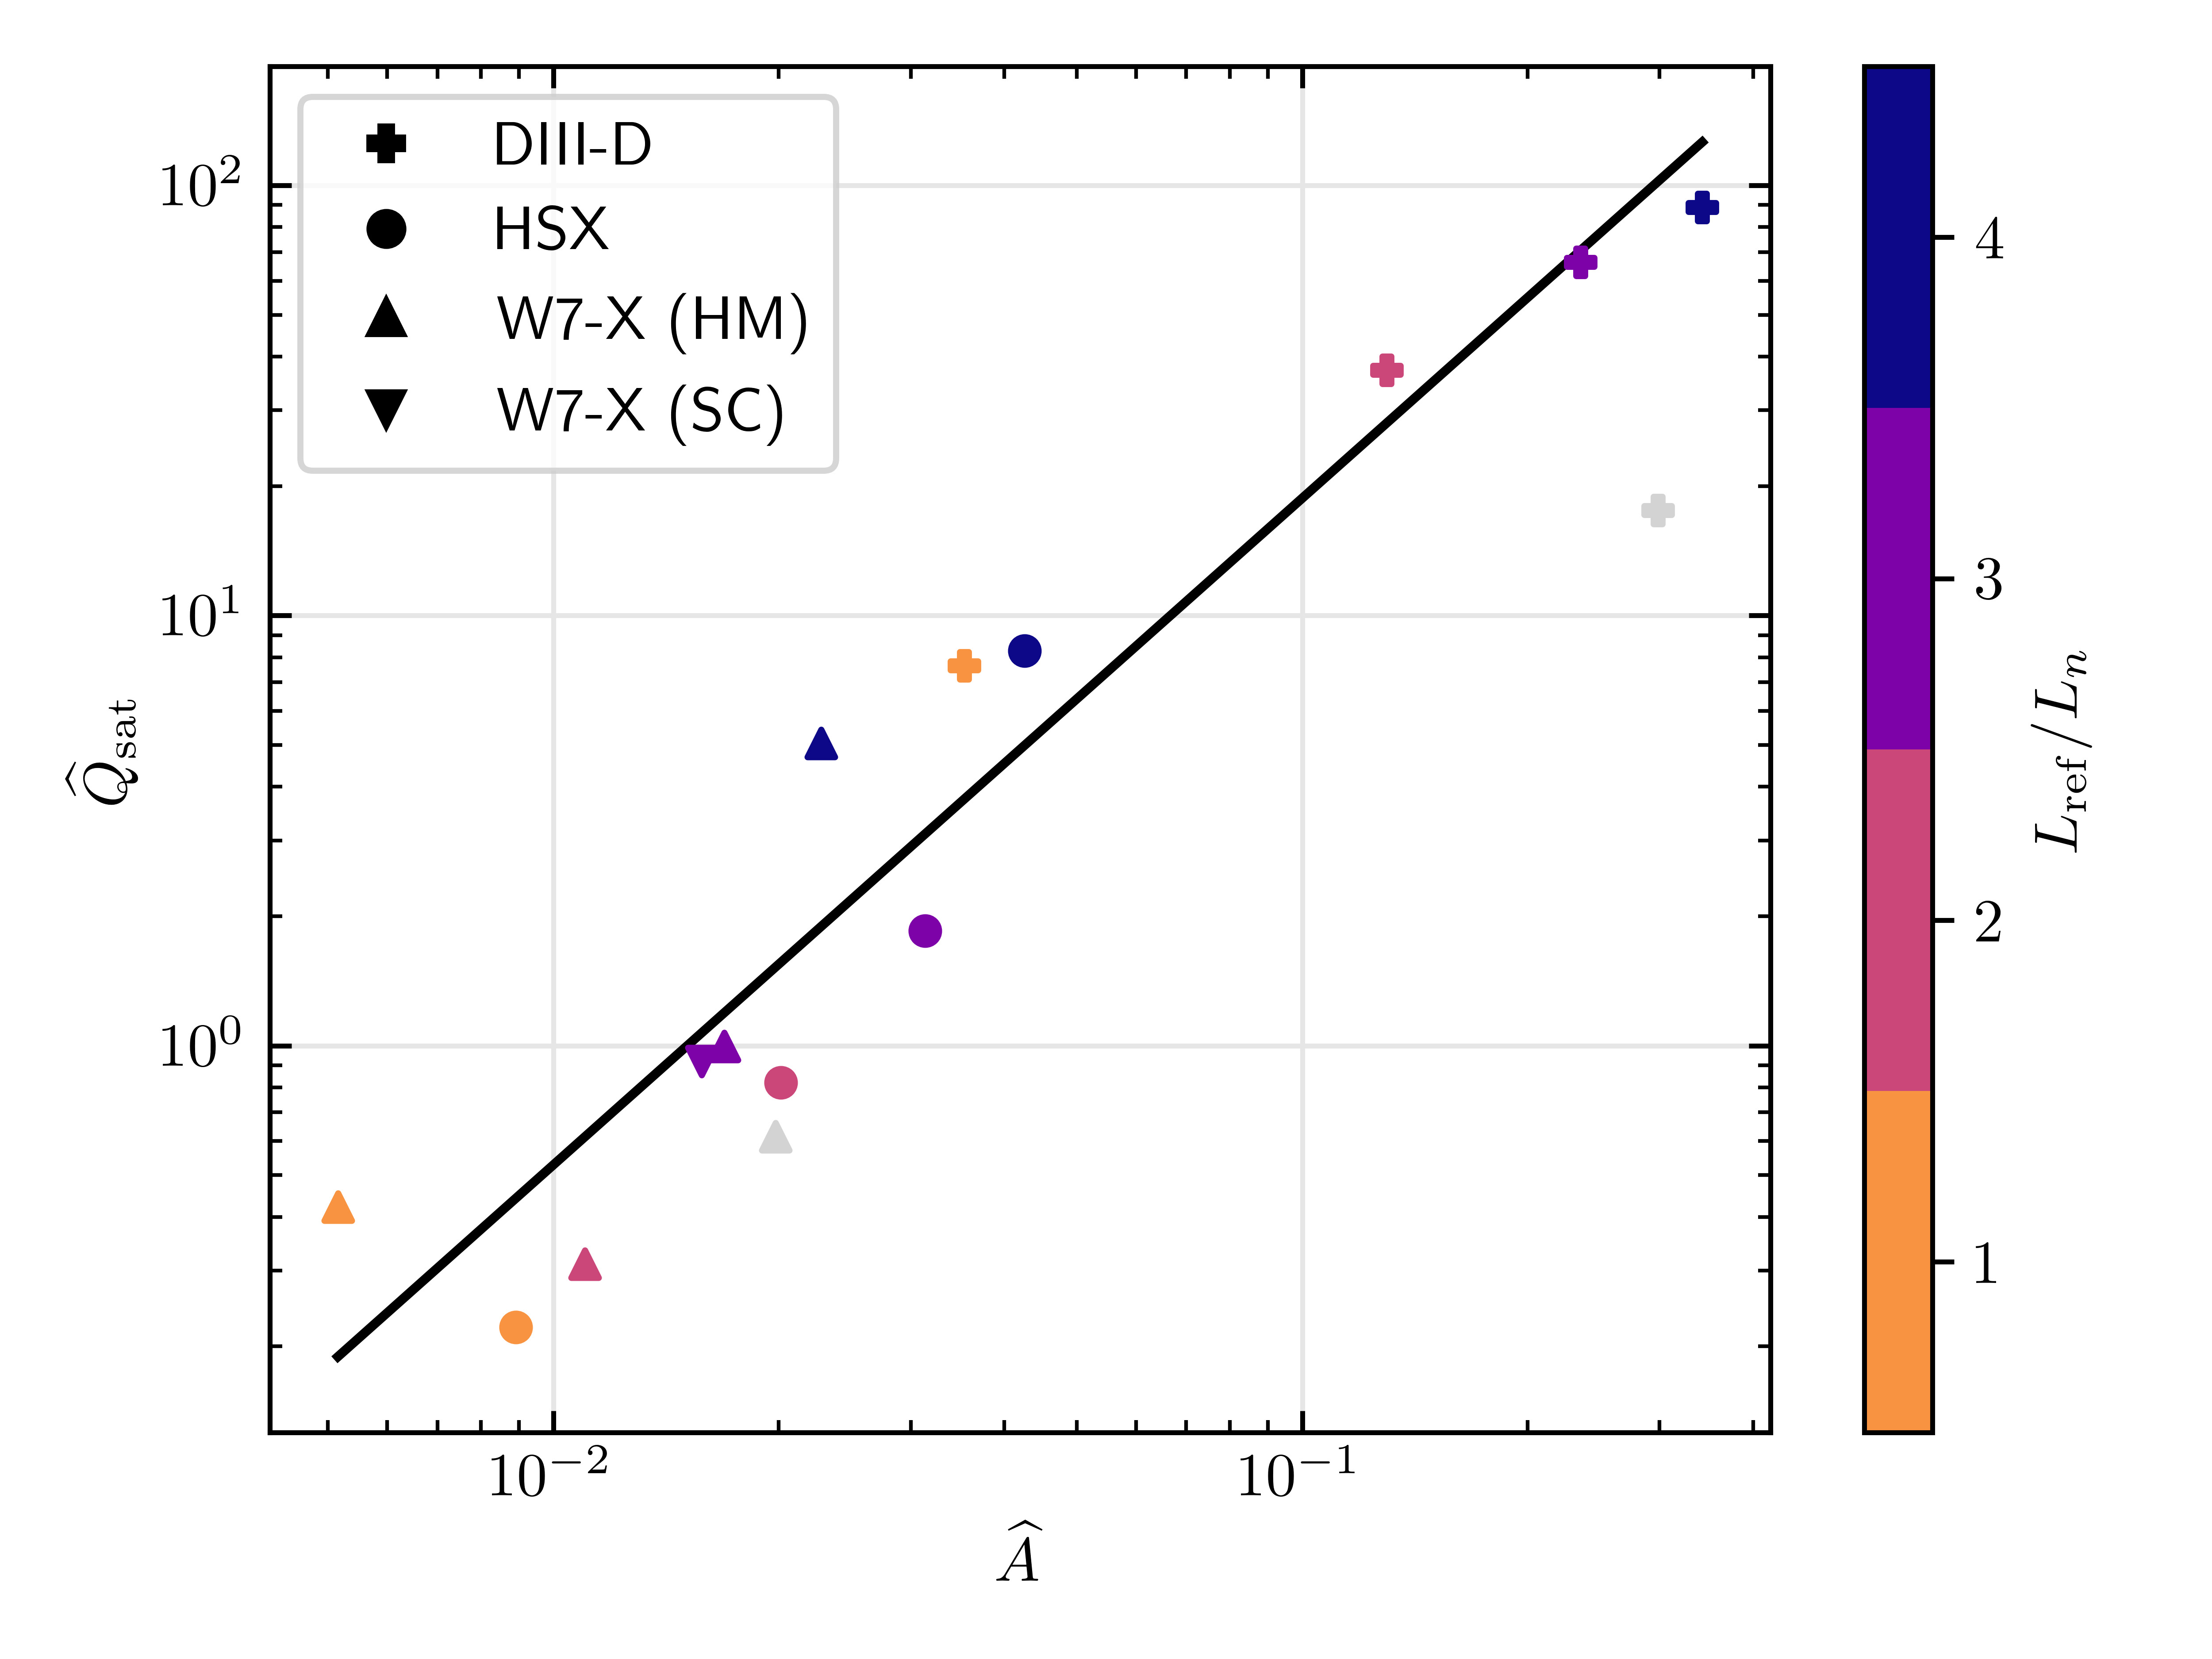
\includegraphics{3_chapters/1_papers/AE-TE/figures/plot_AE_Q_corr.png}
    \caption{A scatter plot showing the normalized \AE{} for a range of stellarator and tokamak plasmas and the average nonlinear saturated turbulent radial energy flux from gyrokinetic simulations of these plasmas. The different points refer to different density gradients, as indicated by the colour, and to different devices. The devices that are used in this analysis are the tokamak DIII-D, the Helically Symmetric eXperiment (HSX), and the W7-X stellarator in both high mirror configuration (HM) and standard configuration (SC). The straight black line shows the least-squares fit, which results in the power law $\ln Q_\text{sat} \propto (1.5 \pm 0.1) \ln A. $}
    \label{fig:scatter_plot_AE}
\end{figure}
A power law is found by fitting a straight line to the log-log plot given in Fig. \ref{fig:scatter_plot_AE}, where we have excluded the grey points from the fitting procedure. The fit results in
\begin{equation}
    Q_\text{sat} \propto A^{1.5 \pm 0.1}.
\end{equation}
This relation is of interest, as it can be motivated in the following manner. The electron energy flux density in the direction of $\nabla x$ is defined as
\begin{equation}
    \begin{aligned}
        {Q}_e &= \frac{1}{V_\text{sim}} \int \epsilon f_{e1} (\boldsymbol{v}_D \cdot 
        \rho\nabla x) \mathrm{d} \boldsymbol{x}.
    \end{aligned}
\end{equation}
Here, $\boldsymbol{v}_D$ is the gyro-averaged drift velocity, and $f_{e1}$ is the fluctuating part of the electron distribution function \citep{Gorler2010MultiscaleMicroturbulence}. We go on to crudely estimate this flux as
\begin{equation*}
    Q_e \sim \sqrt{\langle \mathbf{v}_D^2 \rangle} \int \epsilon f_{e1} \, \mathrm{d} \boldsymbol{x},
\end{equation*}
where the angular brackets denotes an average over the simulated volume.
The integral in this expression is bounded by the \AE{}, and hence we set $\int \epsilon f_{e1} \mathrm{d} \boldsymbol{x} \sim A$. The average of the squared drift velocity,
\begin{equation*}
    \langle \mathbf{v}_D^2 \rangle = \left\langle \left( \mathbf{E} \times \mathbf{B} / B^2 \right)^2 \right\rangle,
\end{equation*}
is proportional to the gyrokinetic energy of the electric field. Since the sum total of the thermal and this field energy should be conserved \cite{Helander2017AvailablePlasmas}, this field energy is also bounded by the \AE{}. We thus estimate that $\langle \mathbf{v}_E^2 \rangle \sim A$, which gives
\begin{equation}
    Q_e \propto A^{3/2},
\end{equation}
in agreement with the observed power-law. We have furthermore tried different conditions for particles which cross the computational boundary \citep{mackenbach2023bounceaveraged}, and we find that the results are resilient against these such variations. \par 
The two grey points lie significantly below the black line in Fig.~\ref{fig:scatter_plot_AE}. A possible reason may be that all the other points refer to plasmas with a density gradient, in which there is, in principle, \AE{} in both the electron and ion populations (although we have only considered the electons). In contrast, for the grey points correspond to plasmas with an electron gradient alone, implying that the \AE{} from the ions vanishes identically. There is thus less energy to drive turbulence in this case. 

\subsection{The distribution of \AE{}}
We now go on to investigate how different trapped particle orbits contribute to the \AE{}. In order to do so, we define an \AE{} per trapping well, namely
\begin{equation}
    \begin{aligned}
        \widehat{A}_\lambda(\lambda) = \int_0^\infty & e^{-z} z^{5/2}  \left[ \hat{\omega}_{\alpha}^2 \left( \frac{ \hat{\omega}_{*}^T }{\hat{\omega}_{\alpha}} - 1 +  \hat{F} \right) + \hat{\omega}_{\psi}^2 \left( -1 + \hat{F} \right)  \right] \hat{G}^{1/2} \mathrm{d}z,
    \end{aligned}
    \label{eq:ae-per-lam}
\end{equation}
so that $\int \sum_{\mathrm{wells}} \widehat{A}_\lambda \mathrm{d} \lambda = \widehat{A}$.
For any given value of $\lambda$, this quantity can be calculated separately for each trapping well. The  bounce points associated with each $\lambda$, which we denote by $\theta_b$ (with $\theta$ being the poloidal angle, our field-line following coordinate), satisfy 
\begin{equation}
    1 - \lambda \hat{B}(\theta_b) = 0.
    \label{eq:relation-lambda-bounce-points}
\end{equation}
One can then draw a straight line between the two bounce-points of a bounce-well, and one can color that line according to its associated $A_\lambda$. One can furthermore investigate $\hat{\omega}_\alpha$ and $\hat{\omega}_\psi$ as a function of their bounce points. This can be done by realising that both $\hat{\omega}_\alpha$ and $\hat{\omega}_\psi$ can be mapped onto their bounce points using equation \eqref{eq:relation-lambda-bounce-points}, and one can thus investigate how their values depend on the bounce-points.
\par 
A plot displaying the properties of equation \eqref{eq:ae-per-lam} in this way is shown in Fig. \ref{fig:AE_per_bw_D3D} for the case of the DIII-D tokamak with a normalised density gradient $L_\mathrm{ref}/L_n = 3$. Additionally, the binormal and radial drifts are shown as dashed green and dash-dotted blue lines, respectively. For convenience, a black dotted line is also displayed which indicates where $\hat{\omega}_\psi = \hat{\omega}_\alpha = 0$. It can be seen that energy is available over most of the magnetic well. Only the most shallowly trapped particles do not contribute to the \AE{}, as $\hat{\omega}_\alpha$ changes sign for these particles. This is in line with expectations, as the more deeply trapped particles experience ``bad curvature'' only, which in turn drives the TEM unstable \citep{Proll2012ResilienceInstabilities,Helander2017AvailablePlasmas}. The contribution to the \AE{} from the trapped particle orbits is enhanced by the positive magnetic shear in DIII-D \citep{connor1983effect}. The most shallowly trapped particles experience good curvature along most of their trajectories and exert, in contrast to the deeply trapped particles, a stabilising influence. Note that this figure refers to a tokamak, which besides being exactly omnigenous only has a single trapping well. Stellarators generally have many different bounce wells, and non-omnigenous effects arise due to net radial drifts.
\begin{figure}
    \centering
    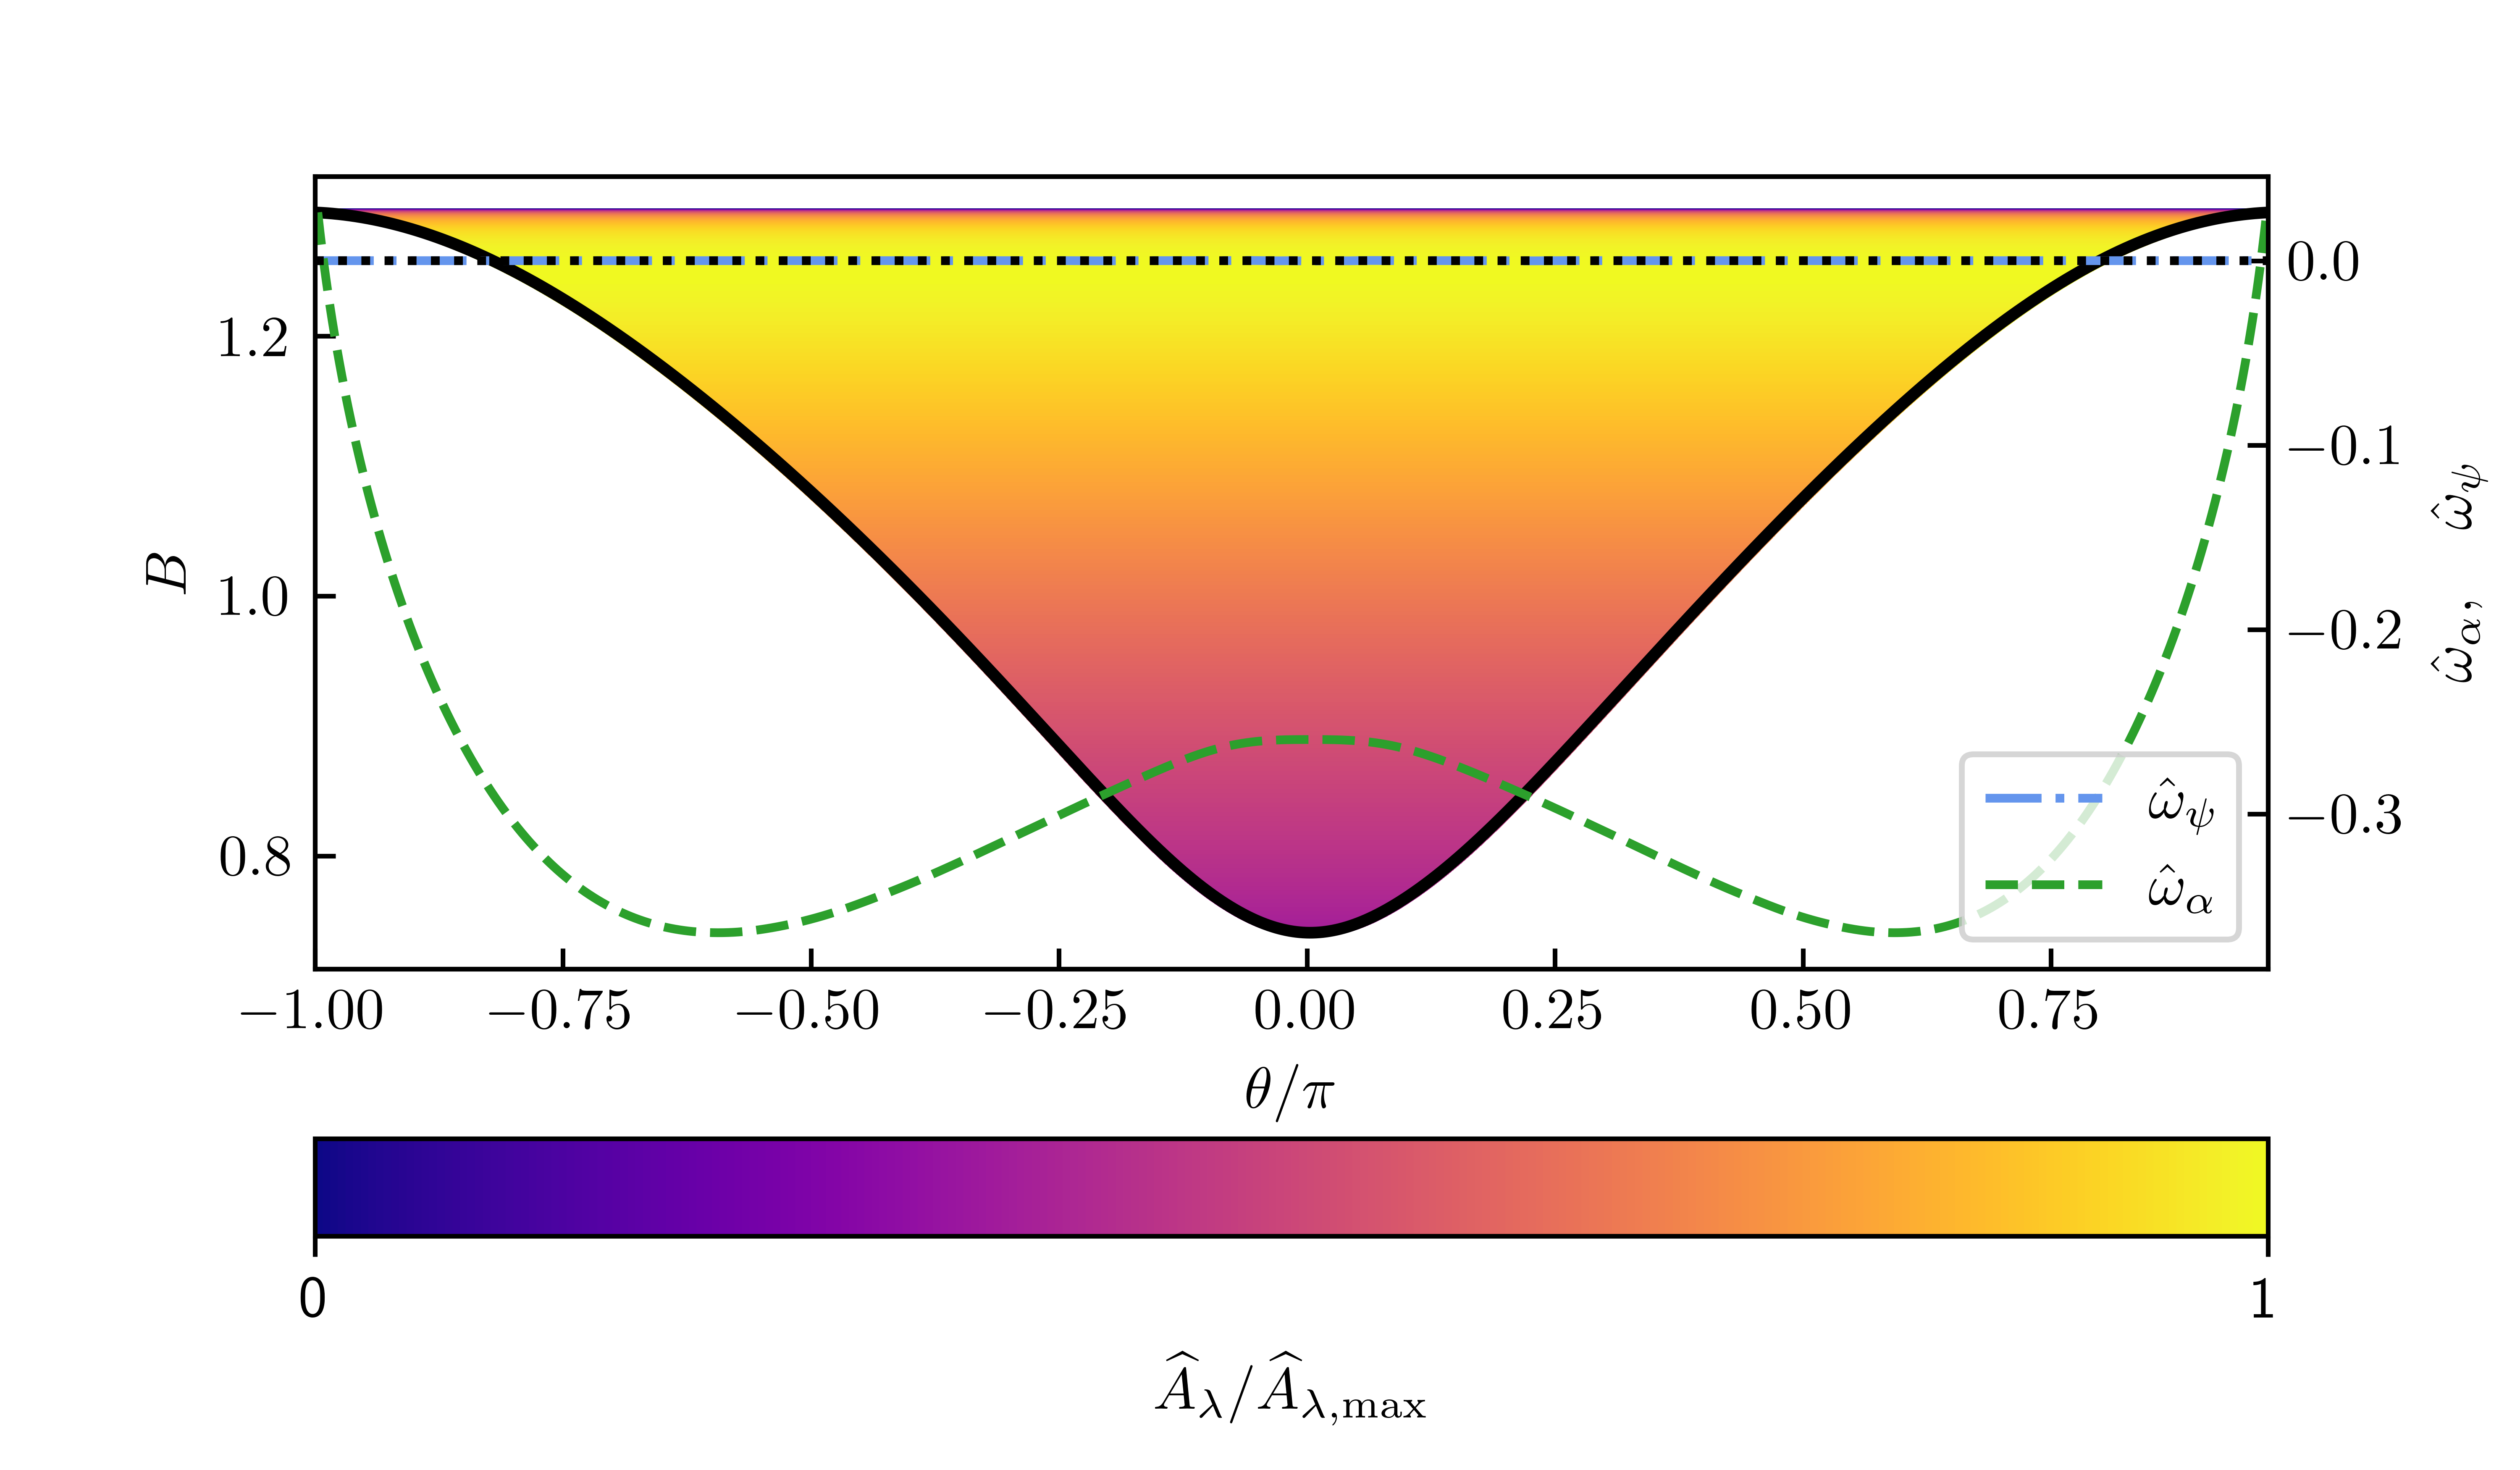
\includegraphics[width=\textwidth]{3_chapters/1_papers/AE-TE/figures/AE_per_lam_D3D.png}
    \caption{The \AE{} per $\lambda$ for DIII-D. The flux tube is located a normalized radial flux of $\psi/\psi_\mathrm{edge}=0.5$.}
    \label{fig:AE_per_bw_D3D}
\end{figure}
\par 
To investigate how these circumstances change the distribution of \AE{} across different bounce wells, we show a plot of W7-X in its standard magnetic configuration in Fig. \ref{fig:AE_per_bw_W7X}, with a density gradient of $L_\mathrm{ref}/L_n = 3$. Several interesting features can be seen. The most pronounced difference to the previous figure is that the \AE{} is much more localized than in DIII-D, so that most of the contribution comes from a narrow range of bounce wells. Most of the \AE{} comes from bright bands in the central well, particularly those where the bounce well approaches the local maximum in $B$ around $\theta = 0$. One can understand this observation in the following manner. Near the local maximum in field strength, the drift is maximally bad (as $\hat{\omega}_\alpha$ is most negative), and the trapped particles in this region contribute significantly to the \AE{}. Furthermore, the \AE{} is weighted by $\hat{G}^{1/2}$, which is proportional to the bounce time, which becomes large near such a local maximum. These two effects combine in the central region, giving rise to the large \AE{} there. One can also see two bright bands at $B \approx 1.10$, which at first seems puzzling as the particles experience average good curvature in this band as indicated by the positive sign of $\hat{\omega}_\alpha$. However, these particles experience a net radial drift ($\hat{\omega}_\psi \neq 0$) and this non-omnigenity causes the \AE{} to be non-zero. Furthermore, it is exacerbated by the large bounce time, resulting in the bright bands seen in the figure. Finally, one can see that, as in a tokamak, shallowly trapped particles barely contribute to the \AE{}, though the fraction of trapped particles which do not contribute is significantly larger than in DIII-D. \par
\begin{figure}
    \centering
    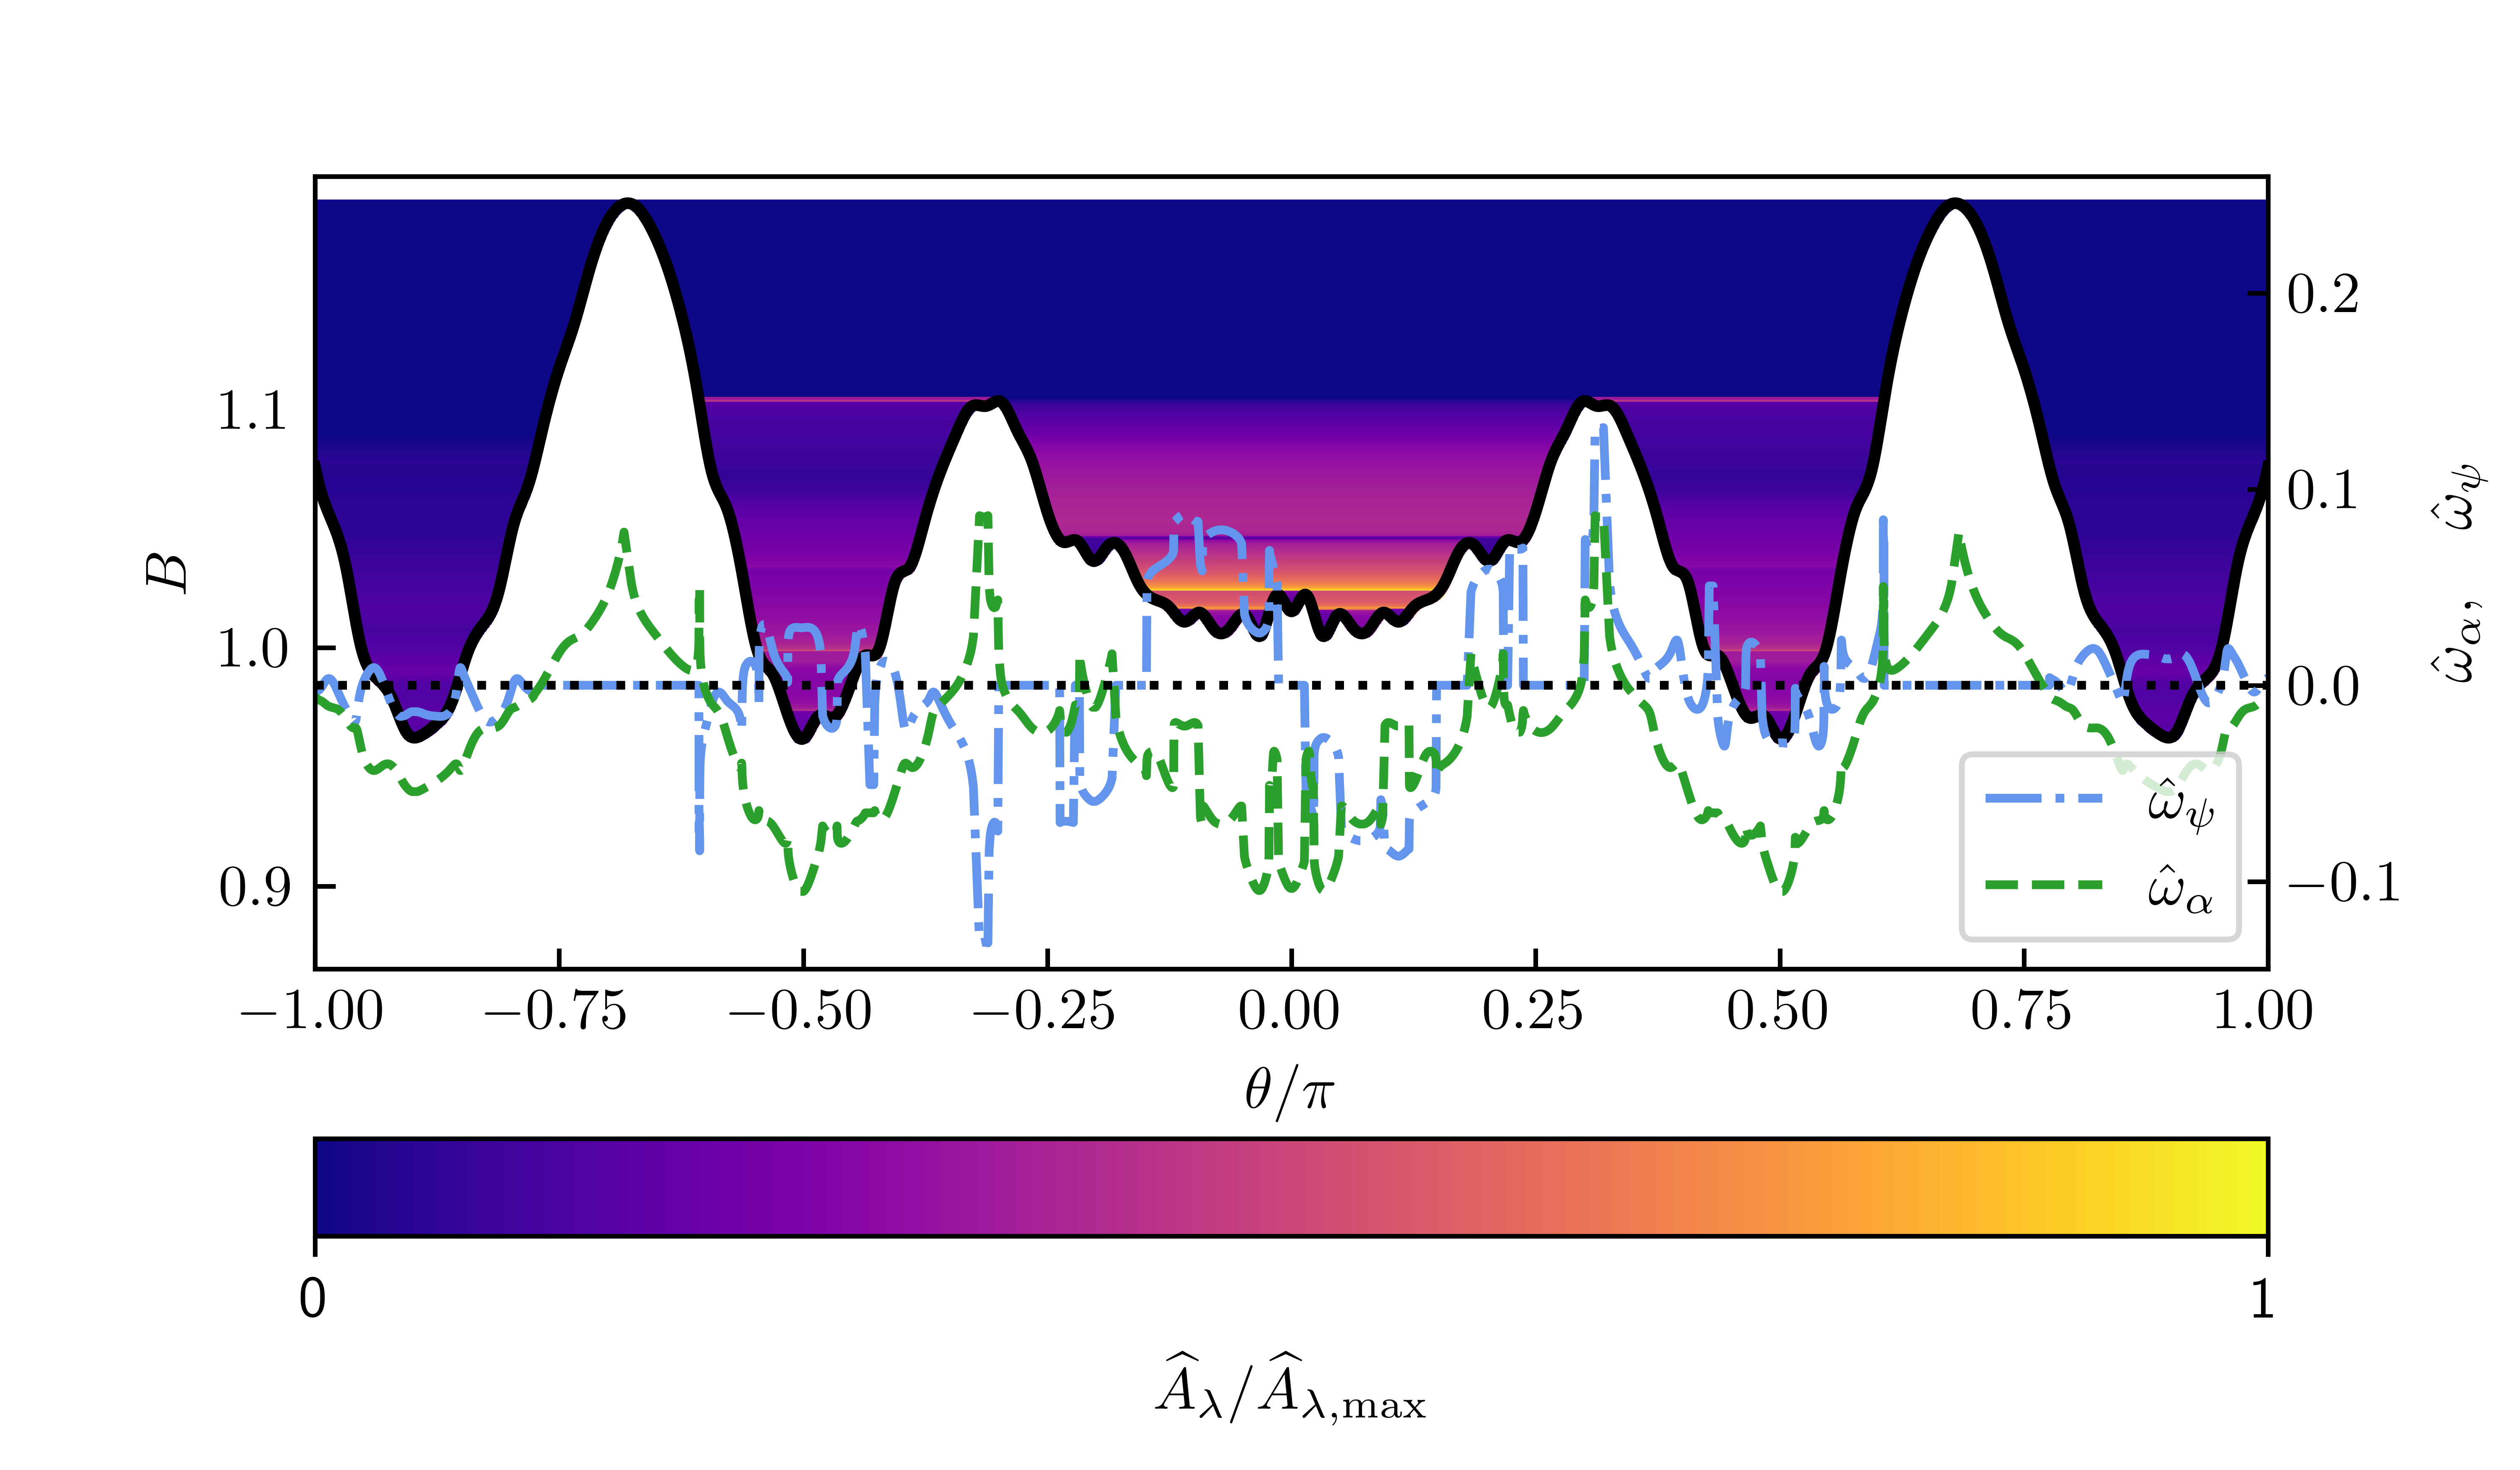
\includegraphics[width=\textwidth]{3_chapters/1_papers/AE-TE/figures/AE_per_lam_W7XSC.png}
    \caption{The \AE{} per $\lambda$ for W7-X (SC). The flux tube is located a normalized radial flux of $\psi/\psi_\mathrm{edge}=0.5$.}
    \label{fig:AE_per_bw_W7X}
\end{figure}
In summary, the distribution of \AE{} across various bounce wells indicates that it is the deeply trapped particles in regions of bad curvature which tend to be most destabilizing. Furthermore, the bounce-time plays an important role in determining which particles contribute most to the \AE{}. Finally, we note that non-omnigenous effects can destabilize otherwise stable regions.
\subsection{Dependence on gradient strength}
We finally investigate how the \AE{} depends on the strength of the gradient $\hat{\omega}_*^T$, when all other variables are kept constant. In the limit of large gradients, it is easy to see that equation \eqref{eq:normalized-AE-final} implies a linear scaling with the gradient strength. We go one step further and expand the integrand around large $\omega_*^T$, which gives
\begin{equation}
    \widehat{A} \propto  \hat{\omega}_*^T \left (\hat{\omega}_\alpha + \mathrm{sgn}(\hat{\omega}_*^T) \sqrt{\hat{\omega}_\alpha^2 + \hat{\omega}_\psi^2} \right) \hat{G}^{1/2},
\end{equation}
where $\mathrm{sgn}(x)=x/|x|$ is the sign function. In the opposite limit of small gradients, we find an important distinction between omnigenous and non-omnigenous devices. In a non-omnigenous device, one can expand equation \eqref{eq:AE-per-total-energy} around small $\hat{\omega}_*^T$, and one finds that in a weakly driven regime the integrand becomes
\begin{equation}
    \widehat{A} \propto (\hat{\omega}_*^T)^2 \frac{\hat{\omega}_\psi^2}{\hat{\omega}_\alpha^2+\hat{\omega}_\psi^2} \hat{G}^{1/2}
\end{equation}
For an exactly omnigenous device, however, this result vanishes due to the factor $\hat{\omega}_\psi^2$. To find the correct scaling for such devices, we return to the expression for the \AE{} of an omnigenous device first found in \cite{Helander2020AvailablePlasmas}. Here it was found that the \AE{} is proportional to
\begin{equation}
    \widehat{A} \propto \iint e^{-z} z^{5/2} \hat{\omega}_\alpha^2 R \left[ \frac{\hat{\omega}_*^T}{\hat{\omega}_\alpha} - 1 \right] \hat{G}^{1/2}  \mathrm{d} \lambda \mathrm{d} z,
\end{equation}
where $R[x] = (x + |x|)/2$ is the ramp function. Note that when $\hat{\omega}_*^T$ is small, the ramp function is non-zero in the region where $\omega_\alpha \rightarrow 0$. If we assume there exists a point where $\omega_\alpha=0$ we can expand around the point $\hat{\omega}_\alpha(\lambda_0) = 0$, and set
\begin{equation}
    \hat{\omega}_\alpha \approx \hat{\omega}_\lambda (\lambda - \lambda_0).
\end{equation}
Next we find the region where the argument of the ramp function is positive by finding where the argument vanishes,
\begin{equation}
    \frac{\hat{\omega}_*^T}{\hat{\omega}_\alpha} - 1 = 0 \implies \lambda \approx \lambda_0 +  \frac{\hat{\omega}_*^T}{\hat{\omega}_\lambda}.
\end{equation}
We can now perform the integral over the range $\lambda \in [\lambda_0,\lambda_0+ \hat{\omega}_*^T/\hat{\omega}_\lambda]$, and we find that the \AE{} to leading order is proportional to
\begin{equation}
    \widehat{A} \propto \int e^{-z} z^{5/2} \hat{\omega}_\lambda \hat{\omega}_*^T \left( \frac{\hat{\omega}_*^T}{\hat{\omega}_\lambda} \right)^2  \hat{G}^{1/2}(\lambda_0) \mathrm{d}z.
\end{equation}
Thus we conclude that, for weakly driven omnigenous devices, the \AE{} integrand scales as
\begin{equation}
    \widehat{A} \propto |\hat{\omega}_{*}^{T}|^3 \frac{\hat{G}^{1/2}(\lambda_0)}{|\hat{\omega}_\lambda|}.
\end{equation}
Hence in summary we have
\begin{equation}
\widehat{A} \propto
    \begin{cases}
        (\hat{\omega}_*^T) & \text{if } |\hat{\omega}_*^T| \gg 1 \\
        ( \hat{\omega}_*^T)^2 & \text{if } |\hat{\omega}_*^T| \ll 1 \text{ and } \hat{\omega}_\psi \neq 0 \\
        ( \hat{\omega}_*^T)^3 & \text{if } |\hat{\omega}_*^T| \ll 1 \text{ and } \hat{\omega}_\psi = 0
    \end{cases}
\end{equation}
\par 
\begin{figure}
    \centering
    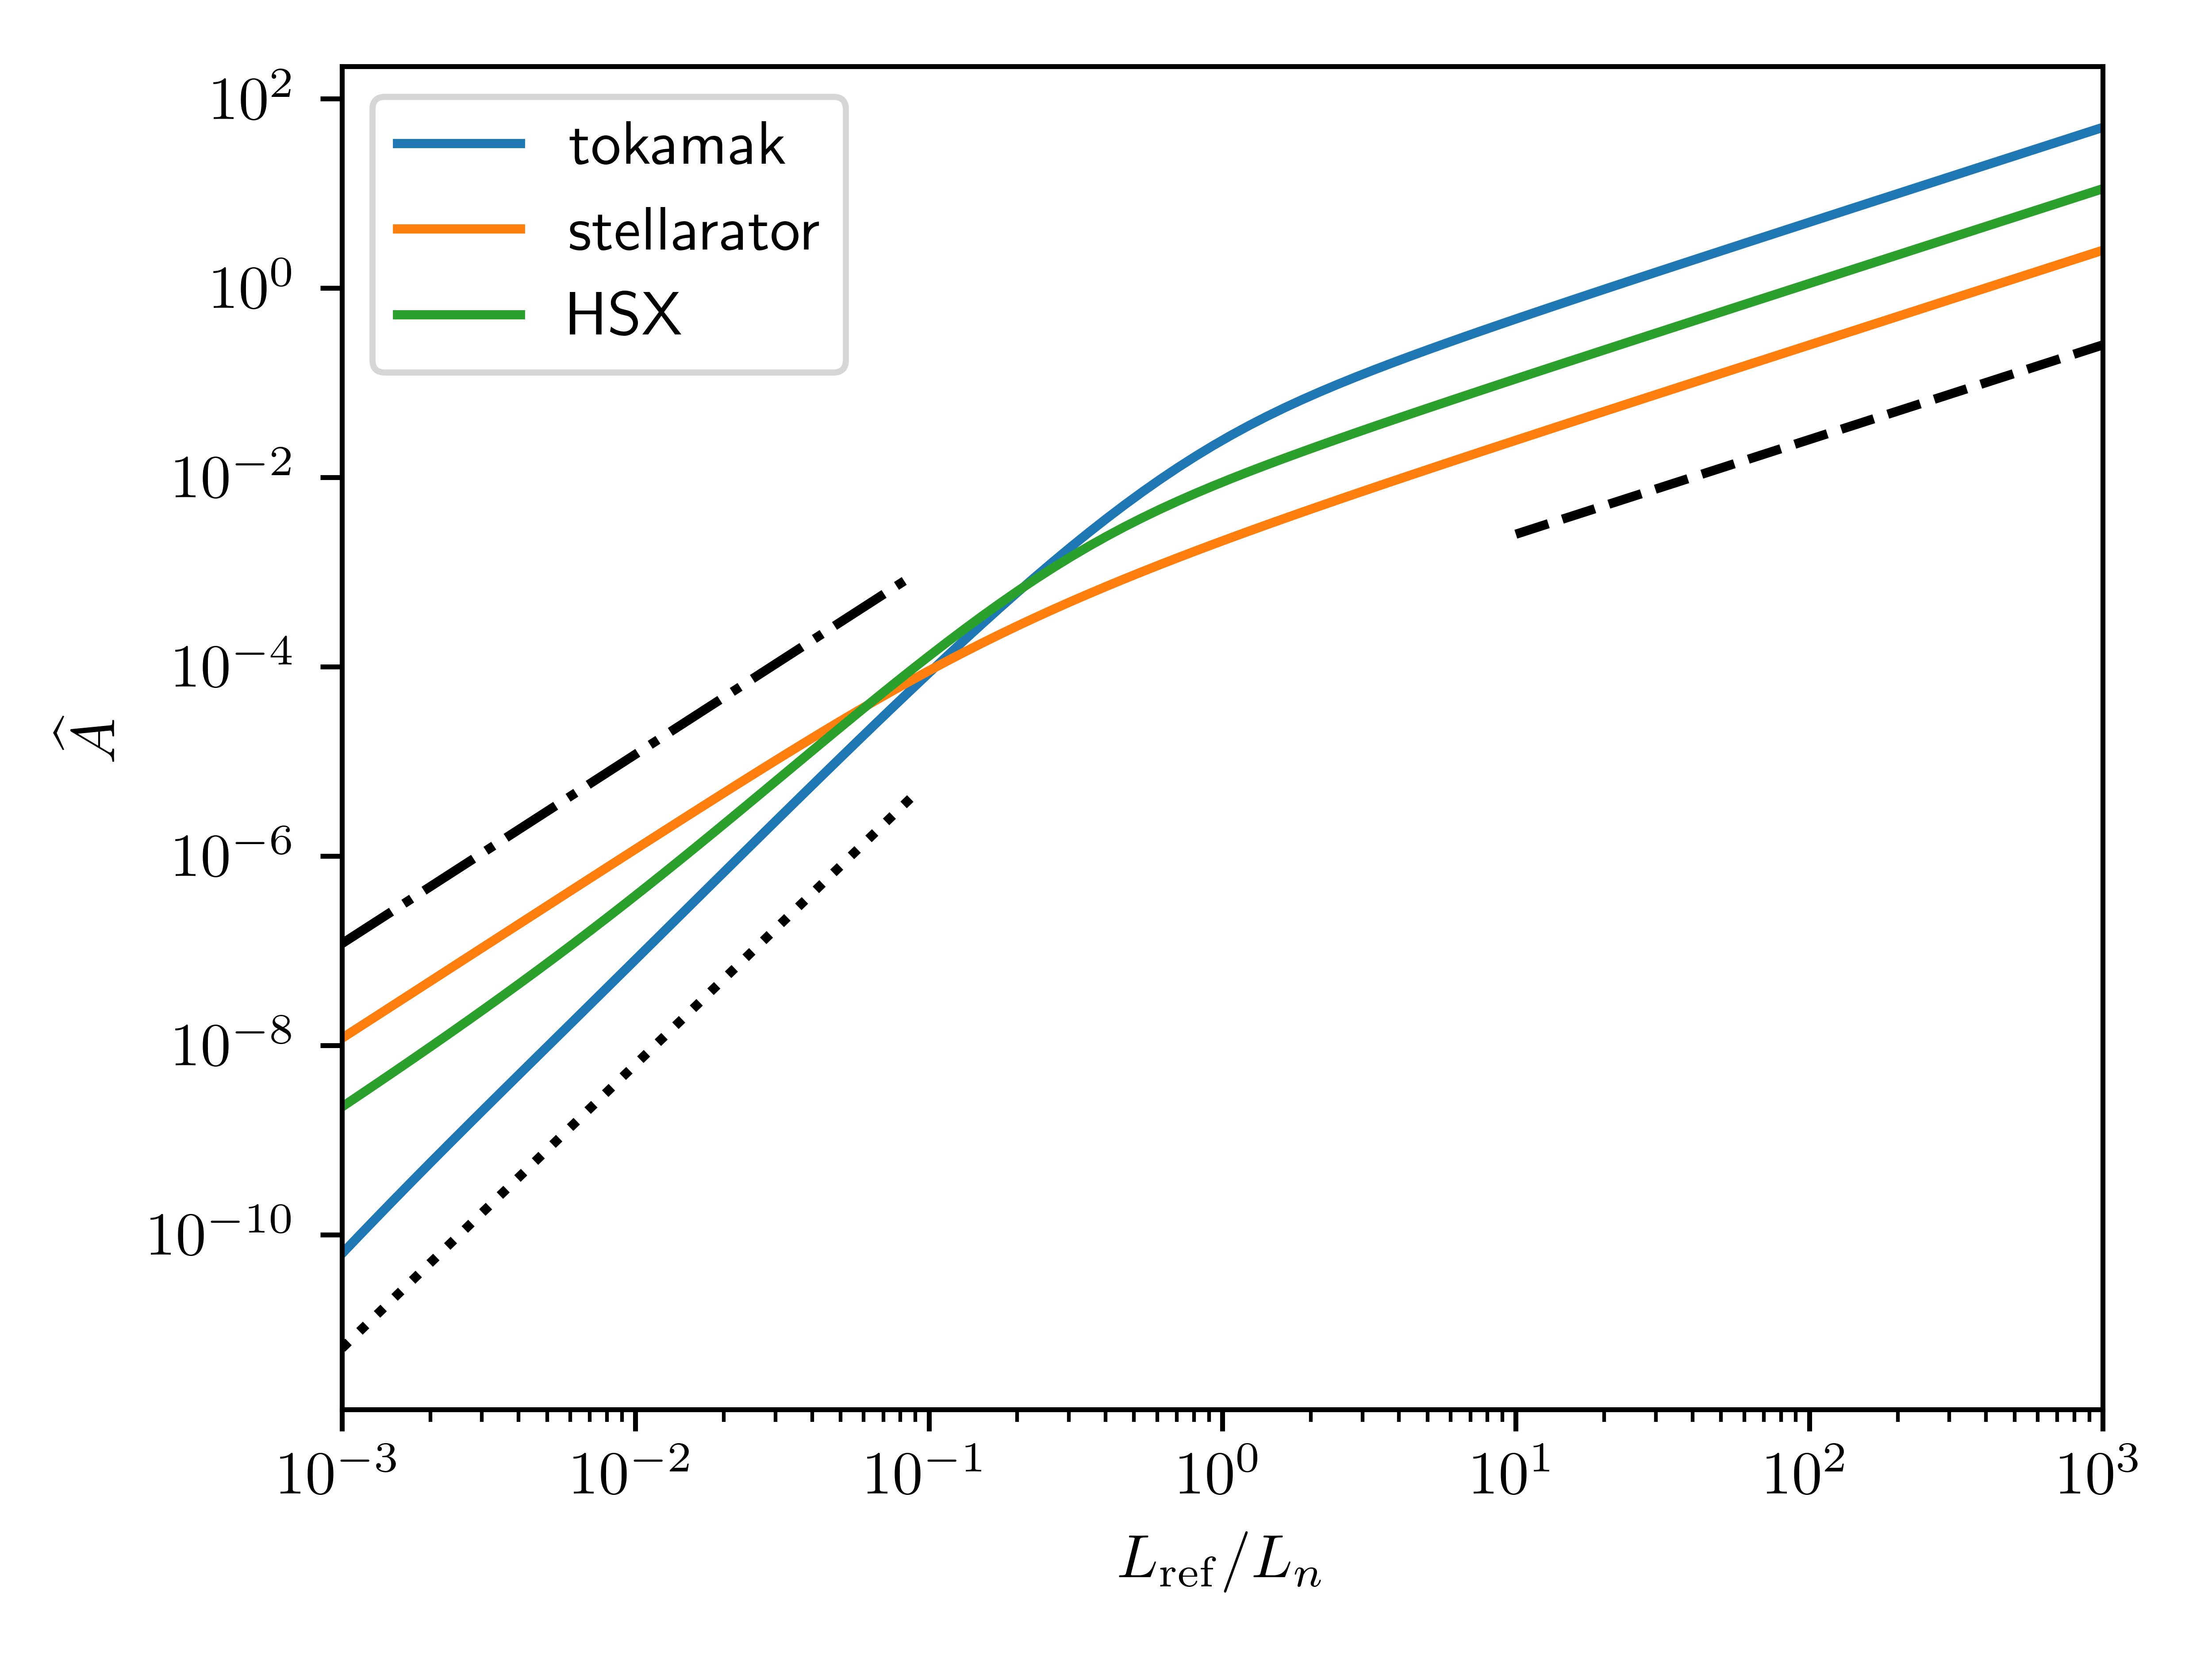
\includegraphics{3_chapters/1_papers/AE-TE/figures/gradient-scaling.png}
    \caption{An example of the dependence of \AE{} on the gradient strength for three different devices; a tokamak, a non-omnigenous stellarator, and HSX. In the case displayed above, the electron temperature gradient is set to zero. The dashed, dash-dotted, and dotted lines have a linear, square, and third power scaling with the density gradient, respectively}
\label{fig:scaling-laws}
\end{figure}
The different scaling laws are displayed in Fig. \ref{fig:scaling-laws}, where we see a tokamak (which is exactly omnigenous), a non-omnigenous stellarator, and the optimized, fairly omnigenous, HSX stellarator. The plots show a distinct ``knee'' at the transition from one scaling law to the next. This knee is especially pronounced for the tokamak, and less so for the stellarator. The difference in scaling for weakly and strongly driven regimes is interesting, as the behaviour is reminiscent of gradient-threshold (also called critical-gradient) type behaviour. Such a gradient-threshold is signified by small transport up to some threshold in the gradient followed by strong transport above this threshold \citep{Dimits2000ComparisonsSimulations}, a behaviour shared by the present plot. It is thought that this critical gradient plays an important role in profile stiffness, where profiles tend to retain their shape without much sensitivity to the details of the particle/energy sources \citep{garbet2004profile}. It is also interesting to note that, from the different scaling laws for omnigenous and non-omnigenous devices, one would expect the critical-gradient-like behaviour of the \AE{} to be ``softer'' in an non-omnigenous stellarator, as the transition from a quadratic to a linear scaling law is more gradual than that from a cubic one. If this gradient-threshold behaviour of the \AE{} indeed corresponds to the true critical gradient, this would result in profiles being less stiff, which has indeed observed in various stellarators \citep{milligen2008quantifying,sanchez2015self}. Investigating HSX more closely, we see that for very low gradients it follows a quadratic scaling, for moderate gradient it approaches a third-power scaling, and for strong gradient it is linear. This third-power region is a result of HSX being close to quasi-symmetry, so that $\hat{\omega}_\psi$ is small. However, at small enough gradients, the $\hat{\omega}_\psi$ term starts to become important causing the scaling to be quadratic. 
\par 
Finally, we note the non-trivial dependence on $\hat{\omega}_\alpha$ in the various regimes. When the gradients are large, the \AE{} is linearly proportional to $\hat{\omega}_\alpha$, which quantifies ``bad curvature'', but for small gradients it is {\em inversely} proportional to $\hat{\omega}_\alpha$. This implies that one can \emph{reduce} the total \AE{} by increasing the amount of bad curvature. This would lead to reduced \AE{} in the weakly driven regime, and the ``knee''-point would be shifted to higher $\hat{\omega}_*^T$, which would lead to a higher critical gradient (as estimated from \AE{}). This is in line with recent results of \cite{roberg2022coarse,roberg2023critical}, who found that the critical gradient can be increased by introducing more bad curvature into the magnetic geometry, which thus leads to  lower turbulent heat-fluxes, though it should be noted that those results concern ion-temperature gradient driven transport. An important corollary of this property is that, in a device with particularly low \AE{} in the weakly-driven regime (much bad curvature), the \AE{} becomes very large in the strongly-driven regime, being linearly proportional to $\hat{\omega}_\alpha$ when $\hat{\omega}_*^T \gg 1$. One can thus either have a device with a high gradient-threshold and low \AE{} for small gradients (which may be attained by increasing the amount of bad curvature), or a device with low \AE{} in the strongly driven regime thanks to relatively little bad curvature in regions with many trapped particles.

\section{Summary and conclusions} 
\label{sec:conclusions}
In this paper we have derived the \AE{} of trapped electrons in a slender flux-tube of magnetically confined plasma, and we have compared it with nonlinear saturated radial electron energy fluxes as calculated by nonlinear gyrokinetic simulations. In deriving the \AE{}, several key insights were required to make progress. Firstly, it was found that the calculation is particularly simple in flux tubes with elliptical cross section. An explicit expression of the ground state can then be found, which was used to calculate the \AE{} to leading order. The result is positive definite, as it must be, and reduces to a previously found expression in the case that the magnetic field is omnigenous. Since the \AE{} depends on the cross section of the flux tube, its major and minor radii need to be chosen a priori. The correct choice depends on the correlation length of the turbulence, which we take to be proportional to the gyroradius in both directions.
\par
We compared the resulting \AE{} for different magnetic geometries with the energy flux computed in a set of simulations of density-gradient driven turbulence. The numerical \AE{} calculations are many orders of magnitude faster than the gyrokinetic simulations. The analysis is done for 4 different magnetic configurations, DIII-D, HSX, and W7-X in its standard and high mirror configurations. The saturated electron energy flux $Q_\text{sat}$ is approximately related to the \AE{} via a simple power law $Q_\text{sat} \propto A^{1.5 \pm 0.1}$. A straightforward phenomenological model to explain the observed power law is proposed, which results in $Q_\text{sat} \propto A^{3/2}$. We go on to investigate which regions are driving the available energy. The results can be understood in terms of simple geometrical concepts: bad curvature (resulting in the drift being in resonance with the drift wave) and non-ommigenity drive \AE{}. We finally investigate the dependence of \AE{} on gradient and find that there are three distinct scaling laws; for strong gradients the \AE{} scales linearly with the gradient strength, whereas for weak gradients the \AE{} scales as the gradient-strength squared or cubed for non-omnigenous or exactly onigenous fields, respectively. 
\par 
These results are interesting for future research. The strong correlation between \AE{} and energy flux across various devices indicates that it may serve as a good proxy-function for stellarator optimisation codes\citep{Spong2001PhysicsStellarators,landreman2021simsopt} used to design stellarators with reduced turbulence. Direct gyrokinetic simulations can be too time-consuming to be carried out inside the optimisation loop in such codes, so there is a need for more efficiently estimating turbulent transport in given magnetic field. It is thus of interest to understand how \AE{} is related to specific details in the field-line geometry. As we have seen, regions of bad curvature are associated with large \AE{}, thus providing a connection between previously known results from linear gyrokinetic stability theory and \AE{}, but the latter also seems to possess predictive qualities for nonlinear transport. Furthermore, one could also use the \AE{} derived here as a profile optimisation tool for TEM-dominated devices. One could then search for plasma profiles and adjustable coil currents which minimize the \AE{}, under some set of constraints. Finally, it may also be valuable to extract expressions for \AE{} in more generic scenarios where turbulence is driven by an ion temperature gradients
\section*{Acknowledgements} \label{sec:acknowledgements}
The authors are grateful for the valuable discussions with, J.M. Duff, J. Ball, T. G\"orler, M.J. Pueschel, P. Mulholland, P. Costello, M.J. Gerard, and E. Rodriguez. This work was partly supported by a grant from the Simons Foundation (560651, PH), and this publication is part of the project ``Shaping turbulence – building a framework for turbulence optimisation of fusion reactors'', with Project No. \texttt{OCENW.KLEIN.013} of the research program ``NWO Open Competition Domain Science'' which is financed by the Dutch Research Council (NWO). This work has been carried out within the framework of the EUROfusion Consortium, funded by the European Union via the Euratom Research and Training Program (Grant Agreement No. 101052200 — EUROfusion). Views and opinions expressed are however those of the author(s) only and do not necessarily reflect those of the European Union or the European Commission. Neither the European Union nor the European Commission can be held responsible for them. 

\renewcommand\thesection{\Alph{section}}
\setcounter{section}{0}

\section{Details of the derivation of the domain shape} \label{app:diff-for-domain}
Here we provide mathematical details for the argument given in Section \ref{sec:theory} concerning the domain shape. 
We do so by means of a geometric argument, sketched in Fig. \ref{fig:proof-of-domain-sketch}. Here $\mathrm{A}$ and $\mathrm{A}'$ denote two points on the boundary with parallel tangents, $T_{\mathrm{A}}$ and $T_{\mathrm{{A}'}}$, respectively. The distance between these tangents is $2D$ and the radius of curvature of the boundary at $\mathrm{A}$ is $R$. If $\mathrm{C}$ is the point on $T_{\mathrm{A}'}$ that is closest to $\mathrm{A}$ we thus have $|\mathrm{AC}|=2D$. Next, we let $\mathrm{B}$ and $\mathrm{B}'$ denote boundary points in the vicinity $\mathrm{A}$ and $\mathrm{A}'$, respectively, such that the tangents through $\mathrm{B}$ and $\mathrm{B}'$ are parallel, and we denote by $\mathrm{E}$ the point on the tangent through $\mathrm{B}'$ that is closest to $\mathrm{B}$. Let us write the distance $|\mathrm{BE}|=2(D+\mathrm{d}D)$ and define $|\mathrm{A}'\mathrm{C}|=2L$. To leading order in smallness of $\mathrm{d} \vartheta$ we have $|\mathrm{DC}|=2D \mathrm{d} \vartheta$. Furthermore, to leading order $|\mathrm{B}'\mathrm{E}|=2L$, implying that $|\mathrm{FE}|=2L\mathrm{d}\vartheta$, where $\mathrm{F}$ denotes the intersection of $\mathrm{BE}$ and $\mathrm{A}'\mathrm{C}$. All in all we find the leading-order relations,
\begin{equation*}
\begin{aligned}
    |\mathrm{BE}|&=|\mathrm{AD}|+|\mathrm{FE}| \\
    2(D+ \mathrm{d}D) &= 2D + 2L \mathrm{d} \vartheta \\
    \frac{\mathrm{d}D}{\mathrm{d}\vartheta} &= L.
\end{aligned}
\end{equation*}
Next we investigate how $L$ changes under some small change $\mathrm{d}\vartheta$. Let us define $|\mathrm{B}'\mathrm{E}|=2L' = 2(L+ \mathrm{d}L)$. Since $|\mathrm{AB}|=|\mathrm{A}'\mathrm{B}'|=R\mathrm{d}\vartheta$ and $|\mathrm{CD}|=2D\mathrm{d}\vartheta$, we have
\begin{equation*}
\begin{aligned}
    2L'&= 2L + 2 R \mathrm{d} \vartheta - 2D\mathrm{d}\vartheta \\
    \frac{\mathrm{d}L}{\mathrm{d}\vartheta} &= R - D.
\end{aligned}
\end{equation*}
Combining these relations, one finds
\begin{equation}
    \frac{\mathrm{d}^2 D}{\mathrm{d} \vartheta^2} = R - D,
\end{equation}
\begin{figure}
    \centering
    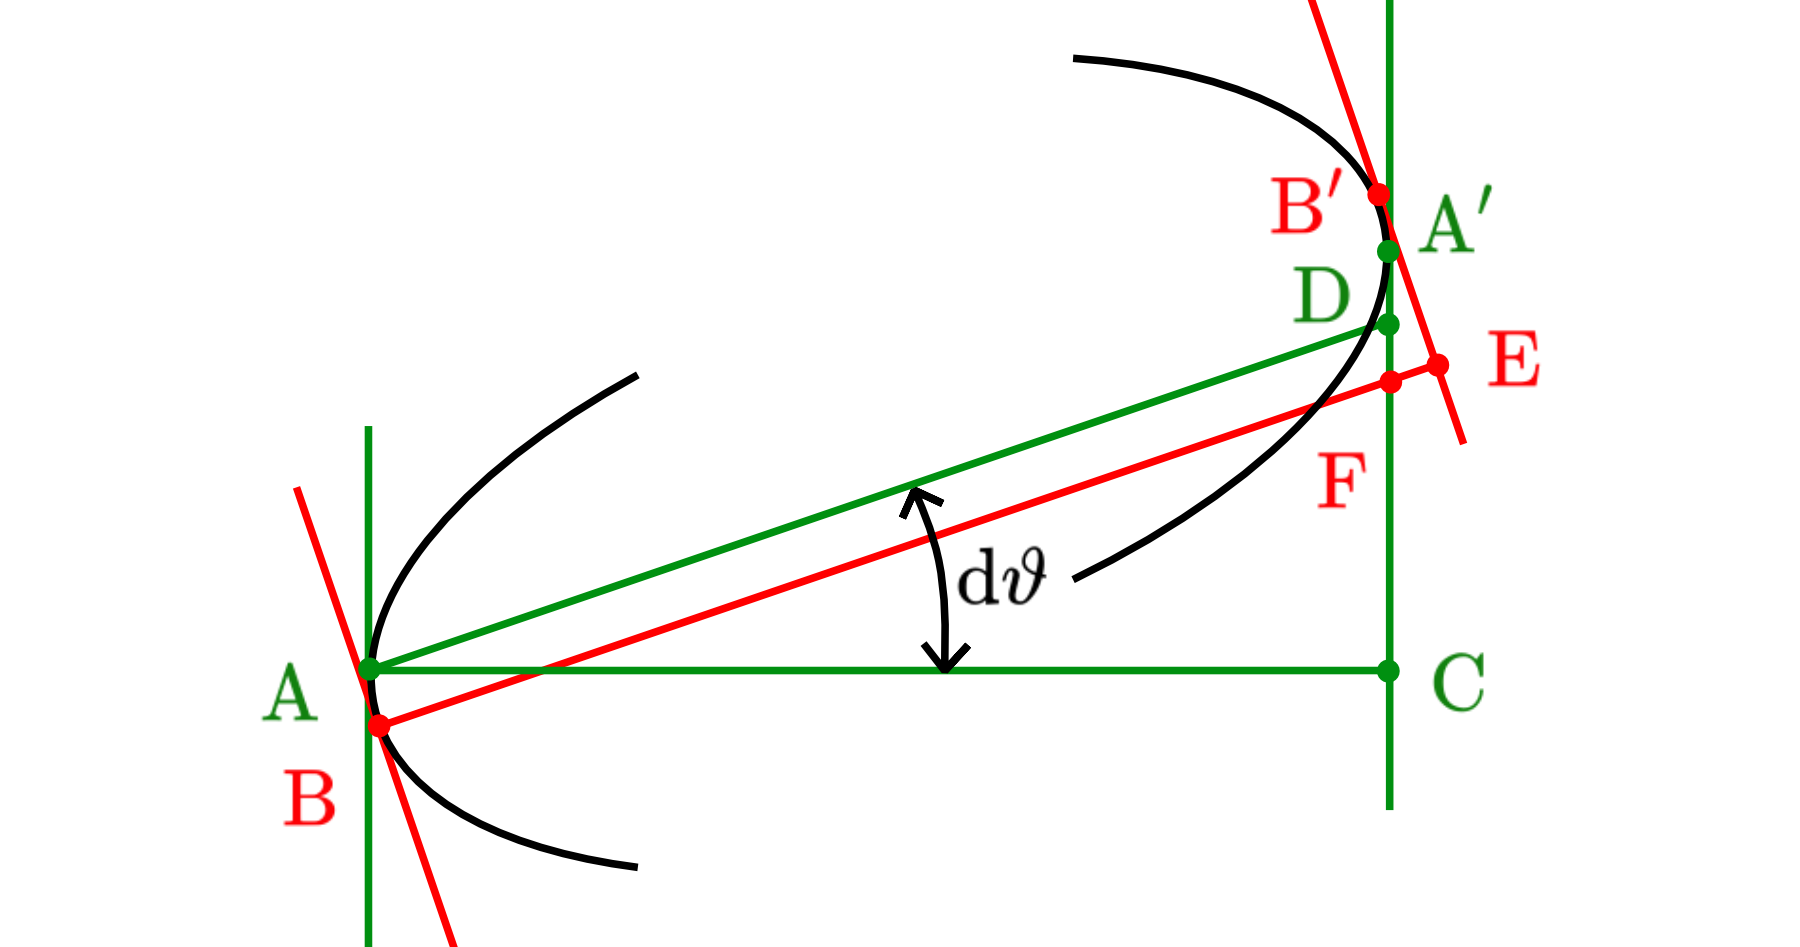
\includegraphics[width=0.8\textwidth]{3_chapters/1_papers/AE-TE/figures/boundary-proof-ellipse.png}
    \caption{A geometric sketch showing the relation between $D$ and $R$. The green vertical lines passing through $A$ and $A'$ are tangent to the boundary, as are the red ones passing through $B$ and $B'$.}
    \label{fig:proof-of-domain-sketch}
\end{figure}
and since $R = C_\mathcal{A}/D^3$ the equation for the domain can be written as
\begin{equation}
    \frac{\mathrm{d} D}{\mathrm{d} \vartheta} = \pm \sqrt{2C - D^2 - \frac{C_\mathcal{A}}{D^2}}.
\end{equation}
It is straightforward to solve for the inverse function, $\vartheta(D)$, which becomes
\begin{equation}
    \vartheta = \int \frac{\mathrm{d}D}{\sqrt{2C-D^2-\frac{C_\mathcal{A}}{D^2}}}
     = \frac{1}{2}\arcsin \left( \frac{D^2 - C}{\sqrt{C^2 - C_\mathcal{A}}} \right) + \mathrm{const.},
\end{equation}
where the integration constant constitutes an unimportant phase, which we can chosen conveniently, e.g., 
\begin{equation}
    D^2 = \sqrt{C^2-C_\mathcal{A}} (C  +\cos 2\vartheta)
\end{equation}
The radius of curvature thus becomes
\begin{equation}
    R(\vartheta) = \frac{C_\mathcal{A}}{(C^2-C_\mathcal{A})^{3/4}(C + \cos 2 \vartheta)^{3/2}}.
    \label{eq:radius-of-curv}
\end{equation}
Our final step is to verify that an ellipse has similar curvature. We first realise that
\begin{equation}
    \tan \vartheta = \frac{\mathrm{d} y}{\mathrm{d}x},
\end{equation}
which for an ellipse, $x^2/a^2 + y^2/b^2 = 1$ implies that 
\begin{equation}
    \tan \vartheta = - \frac{x}{y} \frac{b^2}{a^2}.
\end{equation}
Now, the radius of curvature for an ellipse may be written as
\begin{equation}
\begin{aligned}
    R &= (ab)^2 \left( \frac{\frac{x^2}{a^4} + \frac{y^2}{b^4}}{\frac{x^2}{a^2} + \frac{y^2}{b^2}} \right)^{3/2} \\
    &= \frac{b^2}{a} \left( \frac{1 + \frac{1}{\tan^2 \vartheta}}{1 + \frac{b^2}{a^2\tan^2 \vartheta}} \right)^{3/2} \\
    &=\frac{b^2}{a} \left( \frac{1}{1 + \frac{b^2/a^2-1}{2} (1 + \cos 2 \vartheta )} \right)^{3/2}.
\end{aligned}
\end{equation}
This is of the same form as Eq. \eqref{eq:radius-of-curv}, showing us that the ellipse is indeed the only sufficiently smooth solution to the problem.

\section{Relating derivatives to bounce-averaged frequencies}
\label{sec:appendix-bounce-freq}
Here we show how the derivatives of the energy and distribution function can be related to bounce averaged frequencies. By investigating the bounce-averaged Lagrangian of charged particles in electromagnetic fields, one can derive the following relations \citep{Helander2005CollisionalPlasmas,Helander2014TheoryFields},
\begin{equation}
    \frac{\partial \mathcal{J}}{\partial \alpha} = + q ( \delta \psi ), \qquad \frac{\partial \mathcal{J}}{\partial \psi} = - q ( \delta \alpha), \qquad \frac{\partial \mathcal{J}}{\partial \epsilon} = \tau_b.
\end{equation}
Here $\delta \psi$ is the total excursion in the $\psi$ direction after a full bounce motion, $\delta \alpha$ is the total excursion in the $\alpha$ direction after a full bounce motion, and $\tau_b$ is the bounce time. In general, we know that the second adiabatic invariant can be written as
\begin{equation}
    \mathcal{J} = \mathcal{J}(\epsilon,\psi,\alpha,\mu).
\end{equation}
Taking the total differential of $\mathcal{J}$ we thus find
\begin{equation}
    \begin{aligned}
        \mathrm{d}\mathcal{J}  = \tau_b \mathrm{d}\epsilon - q ( \delta \alpha ) \mathrm{d}\psi + q ( \delta \psi ) \mathrm{d}\alpha + \frac{\partial \mathcal{J}}{\partial \mu} \mathrm{d}\mu.
    \end{aligned}
\end{equation}
This allows us to readily find the derivatives of the energy function. We conclude that
\begin{subeqnarray}
    \left( \frac{\partial \epsilon}{\partial \psi} \right)_{\mu,\mathcal{J},\alpha} &&= + q \frac{\delta \alpha}{\tau_b} \equiv +  q\omega_\alpha, \\
    \left( \frac{\partial \epsilon}{\partial \alpha} \right)_{\mu,\mathcal{J},\psi} &&= - q \frac{\delta \psi}{\tau_b} \equiv - q \omega_\psi.
\end{subeqnarray}
With these findings the derivatives of the Maxwellian can readily be evaluated,
\begin{subeqnarray}
    \left(\frac{\partial f_{M}}{\partial \psi}\right)_{\mu,\mathcal{J},\alpha} &&= + q \frac{f_{M,0}}{T_0} \left( \omega_*^T - \omega_\alpha \right), \\
    \left(\frac{\partial f_{M}}{\partial \alpha}\right)_{\mu,\mathcal{J},\psi} &&= + q \frac{f_{M,0}}{T_0} \omega_\psi.
\end{subeqnarray}
Here, we have defined the electron diamagnetic drift frequency as $\omega_*^T$ as
\begin{equation}
    \omega_*^T \equiv \frac{T_0}{q} \frac{\mathrm{d} \ln n}{\mathrm{d} \psi} \left( 1 + \eta \left[ \frac{\epsilon_0}{T_0} - \frac{3}{2} \right] \right),
\end{equation}
and we have denoted the ratio between the gradients as $\eta = (\mathrm{d} \ln{T} / \mathrm{d} \psi ) / (\mathrm{d} \ln{n} / \mathrm{d} \psi )$.




% \section{The Jacobian of the phase-space reparameterisation}
%  \label{sec:appendix-phasespace-jac}
% Here we derive the Jacobian as we change phase-space variables,
% \begin{equation}
%     \mathrm{d}\boldsymbol{x} = \sqrt{g} \mathrm{d}\psi \mathrm{d}\alpha \mathrm{d}\mu \mathrm{d}\mathcal{J}.
% \end{equation}
% To make matters more convenient, we first calculate the Jacobian for the following transform,
% \begin{equation}
%     \mathrm{d}\boldsymbol{v} = \sqrt{g} \mathrm{d} \mu \mathrm{d}\epsilon.
% \end{equation}
% Firstly note that one can rewrite $\mathrm{d}\boldsymbol{v}$ in the following manner,
% \begin{equation}
%     \mathrm{d}\boldsymbol{v} = \frac{1}{2} \mathrm{d}(v_\perp^2)\mathrm{d}v_\parallel \mathrm{d}\zeta.
% \end{equation}
% Here, $v_\perp$ is the velocity perpendicular to the magnetic field line, $v_\parallel$ is the velocity parallel to the magnetic field line, and $\zeta$ is the gyration angle. We assume our system is independent of the gyration angle (i.e. we can integrate this angle out). We now realize that we can relate the remaining velocity coordinates to our new coordinates in the following manner,
% \refstepcounter{equation}
% \[
%     \mu = \frac{m v_\perp^2}{2 B}, \quad \epsilon = \mu B + \frac{1}{2}mv_\parallel^2. \eqno{(\theequation{\mathit{a},\mathit{b}})}
% \]
% Thus we find that the velocity-space volume element becomes
% \begin{equation}
%     \mathrm{d}\boldsymbol{v} = \frac{B}{\sqrt{\upi}} \left(\frac{2 \upi}{m}\right)^{3/2} \frac{\mathrm{d}\epsilon \mathrm{d}\mu}{ \sqrt{\epsilon - \mu B}}.
% \end{equation}
% We now focus on the real-space part of the transform, $\mathrm{d} \boldsymbol{r}$. We wish to express this real-space part in terms of Clebsch coordinates. We realize that the volume element changes as
% \begin{equation}
%     \mathrm{d} \boldsymbol{r} = \left[(\nabla \psi \times \nabla \alpha) \cdot \nabla \ell \right]^{-1} \mathrm{d} \psi \mathrm{d} \alpha \mathrm{d} \ell.
% \end{equation}
% Now, the magnetic field can be expressed in Clebsch coordinates in the following fashion \citep{Dhaeseleer2012FluxTheory},
% \begin{equation}
%     \boldsymbol{B} = \nabla \psi \times \nabla \alpha = B \frac{\partial \boldsymbol{r}}{\partial \ell}.
% \end{equation}
% Taking the inner product of the above equation with $\nabla \ell$, we thus find
% \begin{equation}
%     (\nabla \psi \times \nabla \alpha) \cdot \nabla \ell = B.
% \end{equation}
% Hence, the total phase-space volume element changes as
% \begin{equation}
%     \mathrm{d}\boldsymbol{x} = \frac{4 \upi}{m^2} \frac{\mathrm{d}\ell}{|v_\parallel|} \mathrm{d}\mu \mathrm{d}\epsilon \mathrm{d}\psi \mathrm{d}\alpha.
% \end{equation}
% We integrate over a bounce motion, giving
% \begin{equation}
%     \mathrm{d}\boldsymbol{x} = \frac{4 \upi}{m^2} \tau_b \mathrm{d}\mu \mathrm{d}\epsilon \mathrm{d}\psi \mathrm{d}\alpha.
% \end{equation}
% Finally, we replace the $\epsilon$ coordinate in favor of $\mathcal{J}$. This gives our final expression for the Jacobian,
% \begin{equation}
%     \mathrm{d}\boldsymbol{x} = \frac{4 \upi}{m^2} \mathrm{d}\mu \mathrm{d}\mathcal{J}  \mathrm{d}\psi \mathrm{d}\alpha.
% \end{equation}


\section*{Competing interests}
The authors declare no competing interests.
%!TEX root = ../../thesis.tex
\chapter[Available energy in tokamaks]{Available energy in tokamaks}
\label{chap: AE-TE}
As we have seen, the \AE{} of trapped electrons showed correlation with gyrokinetic turbulence and as such serves as a useful measure of turbulence transport. There are many possible paths that one could explore now (e.g. optimisation, further generalisation, experimental validation), and several are currently being pursued. An especially fruitful investigation that had been conducted after the found utility of \AE{}, concerns tokamaks. We are interested in finding dependencies of \AE{} on various parameters of interest, e.g., the pressure gradient, magnetic shear, or shape of the flux surface. In tokamaks, these parameters can be varied independently by employing the Mercier-Luc formalism, where the Grad-Shafranov equation is solved locally to a flux surface \cite{MercierLuc1974}, allowing one to assess the impact of the parameters on \AE{}.\footnote{One can employ a similar method to the Mercier-Luc formalism in stellarators, see e.g. \citet{hegna2000local}.} We employ this method in the following paper, which will allow us to make contact with the large body of literature on tokamak research, and one can make both qualitative and quantitative statements concerning the potential benefits of various equilibrium parameters. This is what we do in the following publication.
\vfill \newpage
\includepdf[pages=-,pagecommand={},width=1.1\textwidth]{3_chapters/1_papers/AE-Miller/AE-miller.pdf}


% *************************************************************
%%%% second part
\cleardoublepage
\part{Some observations, conclusions, and outlook}\label{part: closing}
\chapter{Some observations concerning passing electrons}
\vspace*{3mm}
Many generalisations of the \AE{} calculation are possible, and all depend {\it critically} on the chosen invariants, and different choices of invariants have been considered before. The following chapter considers a new, especially natural, generalisation of the results in the current thesis, by investigating passing electrons, and I am grateful for both P. Helander and E. Rodr\'iguez for providing crucial insights here. The generalisation is included, as the calculation of \AE{} is entirely equivalent with only minor interpretative differences.

\section{Invariants on other species}
We have seen in past publications that the \AE{} of trapped electrons serves as a useful measure of gyrokinetic turbulence. Although the research is fruitful, it is lacking in some parts: ions are not accounted for, nor are passing electrons. Thus, it is natural to wonder if \AE{} can be extended to account for these species. One such investigation is presented in \citet{helander2020available}, where the following assumptions are made regarding the various species:
\begin{itemize}
    \item All species obey Liouville's theorem.
    \item Trapped electrons have invariance of $\mu$ and $\mathcal{J}$.
    \item The ions have invariance of $\mu$ alone.
    \item Passing electrons have invariance of $\mu$ and $\psi$.
    \item The electron and ion densities are quasineutral, i.e. the ion charge density exactly balances the electron charge density.
\end{itemize}
The invariance of $\psi$ of passing electrons is motivated by the fast flow of the electrons, which ensures that the radial drift vanishes to the leading order on irrational surfaces \cite{helander2014theory}. However, this constraint is especially restrictive as invariance of $\psi$ makes it impossible to extract energy by flattening the gradient and \AE{} vanishes exactly. However, we know that there may be situations where passing electrons can contribute to various instabilities \cite{jenko2000electron,landreman2015universal,helander2015universal,hardman2022extended,costello2022universal}. Let us somewhat weaken the assumptions imposed on these passing electrons, and there is an especially natural choice one can make, which naturally extends the research presented in this thesis. 

\subsection*{An equivalent $\mathcal{J}$ for passing particles}
Let us return to Eq. \eqref{eq: euler-lagrange for psi}, the Euler-Lagrange equation for the radial coordinate. Restating the result for convenience, we had found the following relationship
\begin{equation}
    \frac{\mathrm{d}}{\mathrm{d}t}\left( \psi + \frac{m v_\parallel}{q} \boldsymbol{b} \cdot \partial_\alpha \boldsymbol{R} \right) = - \frac{\mu}{q} \partial_\alpha B.
\end{equation}
Integrating between two bounce points (where $v_\parallel$ vanishes), we were able to relate the total radial excursion that a trapped particle makes to derivatives of $\mathcal{J}$. Let us now instead consider a passing particle, in a periodic domain (as may be found in a tokamak, or on a rational surface of a stellarator), and we integrate across this domain. Due to this periodicity, we see that
\begin{equation}
    \int_{\rm period} \frac{\mathrm{d}}{\mathrm{d}t} \left( \frac{m \dot{\ell}}{q} \boldsymbol{b} \cdot \partial_\alpha \boldsymbol{R} \right) \mathrm{d} t = 0,
\end{equation}
and, using $E = \mu B + m v_\parallel^2/2$, the Euler-Lagrange equation becomes
\begin{equation}
    q\Delta \psi = \partial_\alpha \int_{\rm period} m v_\parallel \mathrm{d} \ell \equiv \partial_\alpha \mathcal{J}_{p}.
\end{equation}
Therefore, we have found that a passing equivalent of $\mathcal{J}$ behaves entirely analogously to the trapped one. For the binormal coordinate, one finds
\begin{equation}
    q\Delta \alpha = - \partial_\psi \mathcal{J}_p,
\end{equation}
and one again finds that the differential $\mathrm{d}\mathcal{J}_p = 0$, showcasing its invariance. \par 
It is thus a natural choice to impose that $\mu$ and $\mathcal{J}_p$ are conserved for these passing particles, and the calculation of \AE{} is completely equivalent to the one presented for trapped particles. The only interpretative difference is that $\omega_\alpha$ and $\omega_\psi$ now refer to the radial and binormal drift \textit{passing} particles experience in one transit of the periodic domain, where the transit time is given by $\partial_E \mathcal{J}_p$. This equivalence similarly implies that the stabilising properties of maximum-$\mathcal{J}_p$ transfer to the passing population, too. Since $\partial_\alpha \mathcal{J}_p \propto \omega_\psi$ is often much reduced (if not zero) for these passing particles, let us focus on the behaviour of $\partial_\psi \mathcal{J}_p$ of these passing particles.

\section{The maximum-$\mathcal{J}_p$ property}
The analysis of the binormal drift of passing particles is made simpler due to the fact that the singular behaviour bounce-averaging integrals exhibit is not present for passing particles. As such, we may simply investigate the expression for the passing adiabatic invariant and take derivatives without further complications. The passing invariant may be written as
\begin{equation}
    \mathcal{J}_p = \sqrt{2 m E }  \int_{\rm period} \sqrt{1 - \lambda \hat{B}} \: \mathrm{d} \ell,
\end{equation}
with $\lambda = \mu B_0/ E$, $B_0$ is some reference magnetic field, and $\hat{B} = B/B_0$. Taking the derivative with respect to $\psi$, one finds
\begin{equation}
    \partial_\psi \mathcal{J}_p = - \sqrt{\frac{m E}{2}} \int_{\rm period} \frac{\lambda \partial_\psi \hat{B}}{\sqrt{1 - \lambda \hat{B}}} \mathrm{d} \ell.
\end{equation}
The derivative with respect to $E$ may similarly be found as
\begin{equation}
    \left( \partial_E \mathcal{J}_p \right)_{\psi,\alpha,\mu} = \sqrt{\frac{m}{2E}} \int_{\rm period} \frac{\mathrm{d} \ell}{\sqrt{1 - \lambda \hat{B}}},
\end{equation}
and the binormal drift hence reduces to
\begin{equation}
    \omega_\alpha = \frac{E}{q} \frac{\int_{\rm period} (1 - \lambda \hat{B})^{-1/2} \lambda \partial_\psi \hat{B} \: \mathrm{d} \ell }{\int_{\rm period} (1 - \lambda \hat{B})^{-1/2} \: \mathrm{d} \ell}.
\end{equation}
We are now in a position to evaluate the drift. Realise that passing particles have $\lambda \in [0,\hat{B}_{\rm  max}^{-1})$, and it is natural to consider the two limiting cases. For well-passing particles (i.e. $\lambda \rightarrow 0$), we find the leading-order expression
\begin{equation}
    \omega_\alpha (\lambda \rightarrow 0) \approx \frac{\lambda E}{q} \frac{\int_{\rm period} \hat{B} \partial_\psi \hat{B} \: \frac{\mathrm{d} \ell}{\hat{B}} }{\int_{\rm period} \hat{B} \: \frac{\mathrm{d} \ell}{\hat{B}}} \approx \frac{\lambda E}{2q} \frac{\langle \partial_\psi \hat{B}^2 \rangle_{\rm fs}}{\langle\hat{B} \rangle_{\rm fs}},
\end{equation}
where we have introduced the flux-surface averaging operator as $\langle \dots \rangle_{\rm fs}$. This expression is similar to the \textit{magnetic well} term, useful for determining magnetohydrodynamic stability \cite{greene1997brief,landreman2020magnetic,rodriguez2023magnetohydrodynamic}. For favorable magnetodhydrodynamic stability properties, one requires that $D_{\rm well} \propto \langle \partial_\psi \ln \hat{B} \rangle_{\rm fs} > 0$ \cite{helander2014theory}. The maximum-$\mathcal{J}_p$ property requires that $q \omega_\alpha >0 \implies \langle \partial_\psi \hat{B}^2 \rangle_{\rm fs} > 0$, and we thus see a correspondence between the magnetic well and the maximum-$\mathcal{J}$ property. More precisely, if one expands $\hat{B}$ around the smallness in its variation, the criteria to leading order are equivalent, and thus there is a synergy between this magnetohydrodynamic stability criterion and the maximum-$\mathcal{J}_p$ property for passing particles. \par 
Let us next investigate a second limiting case, namely the barely passing particles that have $\lambda \rightarrow \hat{B}_{\rm  max}^{-1}$. Such passing particles spend nearly all their orbit time near the global maximum of $B$ on the flux surface, and as such sample $\partial_\psi B$ only at this location. Denoting $\hat{B}(\ell_{\rm max}) = \hat{B}_{\rm max}$, we then have
\begin{equation}
    q \omega_\alpha (\lambda \rightarrow \hat{B}_{\rm  max}^{-1}) = \frac{E}{\hat{B}_{\rm max}} \partial_\psi \hat{B}(\ell_{\rm max}).
\end{equation}
To investigate the sign of $\partial_\psi B(\ell_{\rm max})$, let us consider the following. 
\begin{enumerate}
    \item Assume that $\partial_\psi B(\ell_{\rm max}) < 0 $ for all $\psi$. This implies that there is a point-maximum in $B$, somewhere on the magnetic axis. However, such a point maximum is impossible as a consequence of Earnshaw's theorem \cite{earnshaw1848nature}, and near the magnetic axis one {\it must} have $\partial_\psi B(\ell_{\rm max}) > 0$.
    \item Let us next assume that $B_{\rm max}$ is unique on the flux surface (this excludes, for example, exactly omnigeneous equilibria). If we then assume that $\partial_\psi B(\ell_{\rm max})$ changes sign for some $\psi > 0$, we have again introduced a local point maximum at the point $\partial_\psi B = 0$. This is once again impossible due to Earnshaw's theorem, and as such we find that $\partial_\psi B > 0 $. If we instead assume that $B_{\rm max}$ is not unique but there is a line of constant $B_{\rm max}$, one simply has one ignorable coordinate and Earnshaw's theorem still holds. So, in this case too, barely passing particles are maximum-$\mathcal{J}_p$.\footnote{I wish to stress that this crucial insight was provided to me by Helander and Rodriguez for which I am thankful, and this finding proved crucial in their investigation of the maximum-$\mathcal{J}$ property in quasi-isodynamic systems which will be published soon.}
\end{enumerate}
We have thus found that the barely passing particles are in all scenarios maximum-$\mathcal{J}_p$. \par 
All in all we have investigated two limiting cases. Well-passing particles are maximum-$\mathcal{J}_p$ if the flux-surface average of $\partial_\psi B^2$ is greater than zero (similar to the magnetic well), and barely passing particles are maximum-$\mathcal{J}_p$ due to the impossibility of point-maxima in $B$. Let us then postulate that, if both limiting cases are maximum-$\mathcal{J}_p$, they are connected monotonically in $\lambda$, and thus all particles are maximum-$\mathcal{J}_p$.

\subsection*{An example case: the limit of the large-aspect ratio tokamak}
Let us, as an example case that showcases our findings from the previous section, calculate the drift in a large-aspect ratio tokamak with circular flux surfaces. In such a limit, we know that the arc length relates the geometric poloidal angle $\theta$ via $\mathrm{d}\ell \approx R_0 \mathrm{d} \theta / \iota$, and the magnetic field is $\hat{B} \approx 1 - \frac{r}{R_0} \cos \theta$ \cite{helander2005collisional}. The passing invariant thus becomes
\begin{equation}
    \mathcal{J}_p \approx \frac{R_0}{\iota} \sqrt{2mE} \int_{-\pi}^{\pi} \sqrt{1 - \lambda (1 - \epsilon\cos \theta)} \: \mathrm{d} \theta,
\end{equation}
where we have introduced $\epsilon = r/R_0$. We may readily take derivatives with respect to $\epsilon$ and $H$ to find the drift, and the result to leading order in the smallness of $\epsilon$ is
\begin{equation}
    q \omega_\alpha = \frac{H}{B_0 R_0 r} \left(\frac{2}{k^2} \left[1 - \frac{E(k)}{K(k)} \right] - 1 \right) \equiv \frac{H}{B_0 R_0 r} \mathcal{F}(k).
\end{equation}
Here we have defined the ``passing'' parameter as $k^2 = 2 \lambda \epsilon / ( 1 + \lambda [ \epsilon - 1 ] )$, which is zero for well-passing particles and one for barely trapped particles. Furthermore, complete elliptic integrals of the first and second kind are defined as $K(k) = \int_{-\pi}^{\pi} (1 - k^2 \sin^2 \theta)^{-1/2} \mathrm{d} \theta$ and $E(k) = \int_{-\pi}^{\pi} (1 - k^2 \sin^2 \theta)^{1/2} \mathrm{d} \theta$. \par 
In terms of the previous section, we find that for around $k^2$ the drift is $\mathcal{F}(k \rightarrow 0) \approx k^2 / 8$. For barely passing particles, one finds $\mathcal{F}(1) = 1$, and intermediate values are included in the plot of $\mathcal{F}(k)$ given in Fig. \ref{fig: F(k)}. For the case given here, it can be seen that all particles are indeed maximum-$\mathcal{J}_p$.
\begin{figure}
    \centering
    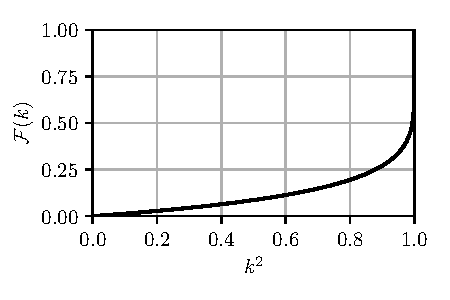
\includegraphics[width=0.6\textwidth]{3_chapters/2_conclusion_outlook/Fk.pdf}
    \caption{The passing particle drift as a function of the parameter $k$.}
    \label{fig: F(k)}
\end{figure}

\section{When is conservation of $\mathcal{J}_p$ relevant?}
Finally, let us consider under what conditions invariance of $\mathcal{J}_p$ is relevant for turbulent transport. The particles should reside in the domain long enough so that turbulence may substantially reorder particles, and one may reach a state akin to a ground state. To be somewhat more precise, the typical residence time of a passing particle in a domain where turbulence resides should be comparable to or greater than typical drift-wave turbulence time scales. Evidently, irrational surfaces break such criteria, as particles sample different field lines with different turbulent structures on them after each transit. Hence a minimal condition one should meet is that the flux surface should be a, preferably low-order, rational surface. In order to ensure that neighbouring surfaces also meet such properties, so that the turbulence may flatten gradients across surfaces, the magnetic shear should similarly not be too large. From the discussion and example given in the preceding sections we have postulated that most equilibria satisfy the maximum-$\mathcal{J}_p$ condition, implying stabilising properties of such low-shear rational surfaces. Such surfaces are often found to be regions where internal transport barriers appear, which are regions with much reduced transport and increased gradients \cite{fujita1997internal,turri2008role,ida2018internal}, although it should be noted that $\boldsymbol{E} \times \boldsymbol{B}$-shearing is thought to play an important role here which the current theory does not account for. \par 
All in all, the above gives a straightforward method of generalising the results in the rest of the thesis to account for passing electrons, with some observations of possible use-cases, using the same tools employed in the rest of the thesis. There are, of course, conditions when the presented method falters. Firstly, one should not expect to accurately model electron-temperature-gradient mode driven turbulence with this method, as both the transit time of the passing electrons and the bounce time of trapped electrons become comparable with the typical turbulence timescales. Hence, only in, e.g. trapped electron mode or ion temperature gradient mode-driven scenarios should one expect this measure to be reliable.

\chapter{Summary, conclusions, \& outlook}
\vspace*{3mm}
In this chapter, we reflect on all that we have learnt from the preceding investigations, what more could be gained from it and where we should proceed with caution. 
\section{Summary}
Taking an eagle-eye's view, we have a desire to better understand and model turbulent transport in plasmas, which is hindered by the complex nonlinear nature of the phenomena involved. A method we employ to tackle this problem is, both philosophically and methodologically speaking, a thermodynamic approach. That is, we make no attempt to describe the precise temporal evolution of the plasma and its constituents, and instead focus on a perspective of energetics and constraints on the system as a whole. This allows one to derive various quantities of interest, such as bounds on nonlinear growth rates of energy \cite{helander2022energetic,plunk2022energetic,plunk2023energetic} or bounds on how much thermal energy can be extracted from the plasma distribution function \cite{gardner1963bound,helander2017available,kolmes2020recovering,helander2020available}, and this thesis focusses on the latter. \par 
This upper bound, called the available energy (\AE{}), depends critically on the constraints imposed on the system. Different constraints result in different answers, and as such, an applicable choice of the constraints is crucial. One especially promising choice of constraints is to impose that the distribution function obeys Liouville's theorem, invariance of the electron magnetic moment, and invariance of $\mathcal{J}$ (often called the second invariant or the parallel invariant). Previous investigations revealed that imposing such constraints aligned with results from the gyrokinetic results of the trapped electron mode, a mode of importance in experiments in both tokamaks and stellarators \cite{rewoldt2005comparison,guttenfelder2008effect,fable2009role}. This makes it a natural candidate to connect the fields of available energy and plasma turbulence, and here we find the inception of the work of this thesis. \par 
In order to accurately calculate the \AE{}, our first course of action was to find precise methods of calculating the various quantities on which \AE{} depends, for which we have constructed a code. These are so-called bounce averages of various functions, for which we construct a numerical framework and create a number of benchmarks by deriving analytical expressions and comparing them against numerical calculations. The framework and benchmarks allow us to assess the performance of various numerical routines, both in terms of accuracy and speed. We found that a straightforward generalisation of the trapezoidal method to calculate the integrals required for such bounce-averages can outperform (in terms of speed) more conventional methods such as quadrature. The code that calculates bounce averages is the basis for the calculations of \AE{}. \par 
We then turned our attention to the problem at hand: finding connections between \AE{} and gyrokinetic turbulence. To ensure that \AE{} models the situation adequately, we first generalised previous results to account for trapped particles that drift radially, so that \AE{} may be calculated in any equilibrium, and found that such radial drifts can significantly affect \AE{} especially if the gradients are small. The generalised \AE{} allowed us to calculate and compare the \AE{} of several stellarator and tokamak equilibria (the DIII-D tokamak, the Helically Symmetric eXperiment, and W7-X) for which nonlinear gyrokinetic turbulence simulations had been performed. There was one important caveat as one had to set a length scale over which energy was available. We argued that this is similar to the length scale over which gradients are flattened; the correlation length. This correlation length is on the order of the gyroradius for micro turbulence, and we thus chose this length scale to be proportional to the gyroradius. Using a simple model for the proportionality factor, namely a constant, we go on to compare the \AE{} with the nonlinear heat flux and found a correlation between the two for trapped-electron-mode dominated electrostatic turbulence simulations, culminating in a power law. This power law could, through a crude argument, be motivated, providing insight into this connection between \AE{} and turbulence. We then turned our attention to the spatial structure of \AE{}, for which we investigated the dependence of \AE{} on the considered bounce well. This allowed us to pin-point which regions of the bounce-well contributed most to the instability of the TEM, and we found that it was typically the deeply trapped particles and regions with trapped particles which drift radially. Therefore, an optimal stellarator (in terms of \AE{}) should have radially stationary trapped particles and be maximum-$\mathcal{J}$ for as many trapped particles as possible. Finally, we investigate the asymptotic behaviour of \AE{} in terms of gradient strength. Here, we identified two distinct regions with different scalings. For weak gradients, we found a sharp decrease in \AE{} with decreasing gradient strength, whereas in a strongly driven regime \AE{} responds linearly to the gradient strength, somewhat reminiscent of gradient threshold-type behaviour. \par
Since the \AE{} showed a connection to turbulent transport, we considered simplified scenarios in which the dependence of \AE{} on various parameters of interest can be investigated. To this end, we specialised the theory in tokamak equilibria, which simplified some of the steps required in the calculation of \AE{}. Furthermore, we specialised the tokamak geometry in a family of equilibria considered by \citet{miller1998noncircular}, which depend on magnetic shear, pressure gradient, and triangularity. The dependence of \AE{} on this set of parameters could then be deduced. We found that negative shear and a high pressure gradient help reduce \AE{}. The dependence on triangularity was found to be more involved, reducing \AE{} only when shear was sufficiently high or when the gradient was sufficiently low. We then estimated a gradient threshold-like quantity from \AE{} and found that this threshold increased with increasing magnetic shear and decreasing triangularity. Next, we optimised the tokamak geometry (i.e. elongation and triangularity) to minimise \AE{} and found that such an optimal geometry is strongly dependent on equilibrium parameters such as magnetic shear and pressure gradient. Going on to consider more experimentally relevant dependencies, we investigated the dependencies of \AE{} on the density gradient, the pressure gradient, and the magnetic shear simultaneously, which are generally coupled via, e.g., bootstrap currents. This allowed us to identify paths in the three-dimensional parameter space of shear, pressure gradient, and density gradient, in which one could increase the density gradient while {\it lowering} the \AE{}. These paths generally required that, as the density gradient increases, the pressure gradient should increase, and the shear should decrease, and we argued that such dependencies are found in experiments. The qualitative difference of the path was strongly dependent on the geometry considered, with the negative triangularity geometry not showing a sharp decrease in \AE{} with increasing density gradient. We finally made an additional comparison with the nonlinear heat flux by means of the \textsc{tglf}-code. This showed a correspondence between the \AE{} and the estimated heat flux, with regions in parameter space where the correspondence is less pronounced. These deviations can be corrected for by improving the model for the proportionality factor in the available energy length scale.  \par 

\section{Conclusions}
With all the results of the publications reiterated, let us return to the central question put forth in the thesis, {\it can \AE{} predict gyrokinetic turbulent transport and can it be used to infer its dependencies?} With the important caveat that we can only make statements on this premise when it concerns trapped electrons, we may now attempt to formulate an answer. \par 
For these trapped electrons, we have found that there is a connection between \AE{} and turbulence, as made clear by the correlation between the heat flux and \AE{}. The correlation found shows that \AE{} is useful as a turbulence measure. By specialising the research to tokamaks, we were able to investigate dependencies on parameters like magnetic shear, pressure gradient, and elongation, which allowed us to compare with the existing literature. This showed a correspondence, for example, with negative shear or large pressure gradients having a decreased \AE{} compared to those with little shear or pressure gradient. We should, however, proceed with caution and stress under what conditions one could expect deviations from the found power law. 
\begin{enumerate}
    \item Returning to the definition of \AE{}, we recall that it represents the maximal amount of thermal energy that may be liberated, and thus provides an upper bound for the turbulent energy. However, the true turbulent state is a dynamic one, and as such {\it cannot} be the stationary ground state. The question then is how dissimilar the dynamic state is from the ground state. The similarities highlighted of turbulence and \AE{} in various publications show that there is similarity, but it is not inconceivable that there are situations in which the dynamic state is very distinct from the ground state. 
    \item Similarly to the previous point, we remind ourselves that there are several stabilising mechanisms present in plasma turbulence, the prototypical example being the zonal flow \cite{diamond2005zonal,itoh2006physics,fujisawa2008review}. Zonal flows are large radial variations in the electrostatic potential, which via $\boldsymbol{E}\times \boldsymbol{B}$ flows stabilise the turbulence. Note that this zonal flow is formed by part of the \AE{} (i.e. it has some energy associated with it), yet it acts {\it stabilising}. More mechanisms have been identified, e.g. perpendicular particle diffusion as shown by \citet{merz2008nonlinear}, and others can be found in Refs. \cite{terry2015overview,pueschel2016stellarator,hegna2018theory,faber2018stellarator}. In a zonal-flow-dominated scenario a na\"ive heat-flux estimate from \AE{} may falter as much of the energy resides in the electric field generating the zonal flow. More broadly speaking, \AE{} is a theory that estimates how much energy is liberated, but it does not account for how the energy is {\it distributed}. 
    \item \AE{} has one free parameter that one cannot set a priori, namely the length scale over which energy is available. We have argued that this should be similar to the perpendicular correlation length, and in general this length scale can depend on equilibrium parameters and may vary. The problem is even more fundamental, as we have only argued that it is similar to the correlation length, but not that it is necessarily the same. As such, finding the correct length scale is an ill-defined question, which, depending on its definition, may have different answers. One attractive option is to define the correlation length to be the length scale that minimises the error between the heat flux and the \AE{} estimate. The length-scale would then play a similar role as the quasilinear weights in codes which estimates heat- and particle fluxes using linear estimates (e.g. QuaLiKiz or {\sc tglf}) \cite{staebler2007theory,casati2009validating,citrin2012quasilinear,staebler2021verification}.
\end{enumerate}
To return to the central question of the thesis, we state that the \AE{} of trapped electrons can predict gyrokinetic turbulence and its dependencies, with some important caveats (stressed above) that one should keep in mind. This is shown by several observations; there is a correlation between \AE{} and heat flux, and \AE{} reproduces known trends in tokamaks. It furthermore exhibits more behaviours similar to turbulence, such as gradient-threshold-like behaviours and unfavorable scalings (i.e. increasing \AE{}) with a lesser degree of omnigeneity.

\section{Outlook}
The research question is now answered, and we look forward to what research can be pursued next. We present this as a list, with the most low-hanging fruit listed first and more exotic research projects presented later.
\begin{enumerate}
    \item {\it Stellarator optimisation:} the most straightforward application of the found results is stellarator optimisation, where one attempts to find the best performing (low turbulent energy losses, good fast particle confinement) stellarator. Previously, evaluating turbulence was impossible due to the high computational cost of such simulations, but with \AE{} it is now practicable. This is attractive for several reasons; the \AE{} penalises lack of radially stationary trapped particles which is a common goal of stellarator optimisation, and the optimisation will try to find maximum-$\mathcal{J}$ configurations (at least for density gradient driven trapped-electron-modes) which has also become a more common goal in optimisation. The attractive property of \AE{} is that it penalises both in a consistent fashion, and it also accounts for different trapped particles (as parameterised by $\lambda$). \AE{} however does not, in its current form, also consistently weigh different flux surfaces, and as such one needs to account for this in some manner (one possible method of doing so may be found in \citet{goodman2022constructing}). We have, of course, seen an attempt at optimisation in a simplified scenario in the investigation into tokamaks, where several important conclusions were drawn; the optimisation depends critically on the various profiles of temperature, density, pressure, and rotational transform. Ultimately, all of these should be calculated self-consistently (such as in the \textsc{trinity}-code \cite{barnes2009trinity,barnes2010direct,highcock2014trinity,highcock2018optimisation}) so that the profiles themselves become part of the optimisation routine.
    \item {\it Further validation:} In the presented investigation we have made various predictions which can be scrutinised to a greater degree. For example, we have seen that at high shear, negative triangularity becomes favourable and should benefit from a reduction in transport, in line with some research. This claim may be tested by means of a gyrokinetic code to investigate if this claim is indeed true in general or, if it falters, to find under what conditions the claim fails. This is also true for claims relating to gradient threshold behaviour: various predictions have been made in terms of how the \AE{}-estimate of this threshold moves, and we have made a connection to past research. The gold standard is a comparison against gyrokinetic codes, an endeavour which should be undertaken.
    \item {\it Generalisation to multispecies plasmas:} Seeing the successful description of the \AE{} of trapped electrons, it is natural to wonder about extensions of the research to account for ions and perhaps even impurities. As stressed multiple times in the thesis, such a generalisation depends critically on the chosen invariants, and these choices non-trivially alter the \AE{}. Appropriate choices are not obvious a priori. If a set of invariants is successfully found, the domain of application of \AE{} can be expanded to account for ion species and passing electron species, too. 
    \item {\it Applications outside of plasma physics:} Although the entire thesis has focused on plasma physics, none of the methodologies presented restricts it to this domain: the first application of \AE{} in physics was meteorology after all \cite{lorenz1955available}. In essence, the only requirement for the methods presented is Liouville's theorem, which many systems obey. A list of such systems is given in the references of \cite{kolmes2020available,mackenbach2022available}, but let us highlight a few of these systems here. One famous example is the Vlasov-Poisson system underlying the dynamics of collisionless self-gravitating matter, in which the potential of the Vlasov-Poisson system is the gravitational potential. In quantum physics, there is a correspondence between Bose-Einstein condensates and Vlasov-Poisson systems, as shown by \citet{mocz2018schrodinger}, and the \AE{} can thus be applied to such systems, too. The framework can hence be extended to these systems, and the problem becomes more interesting by imposing additional invariants.
\end{enumerate}
These possibilities allude to many more fruitful applications of the research presented, but, as always, the proof of the pudding is in the eating. \par 
Let us finally take a step back and place the research in a bigger picture. This research falls into the broader scope of plasma thermodynamics, and this field is blossoming, with many promising results found in the last couple of years \cite{helander2017available,helander2020available,kolmes2020recovering,helander2022energetic,plunk2022energetic,kolmes2022minimum,ewart2022collisionless,plunk2023energetic,ewart2023non}. This is in contrast to more traditional methods, where one investigates the dynamics of plasma systems by researching the (linearised) equations and extracting quantities such as growth rates. This traditional approach approach is, of course, valuable, especially with new advances in machine learning that speed up calculations \cite{hui2021machine,mathews2021turbulent,kube2021machine,ho2021neural,anirudh20222022}. Plasma thermodynamics may then be considered a less-explored complementary approach, where one neglects detailed descriptions of dynamics in favour of bounds. It is here that we may find general insights about fundamental processes in plasmas, and I look forward to seeing the field mature.


%%%% BACK MATTER ***************************************************************
\isstarredchaptertrue           % This state variable is used for creating the thumb index by indicating that the following chapter is not numbered (i.e. \chapter*{})
\bookmarksetup{startatroot}
\addtocontents{toc}{\bigskip}%
%!TEX root = ../thesis.tex
%\footnotesize
{\fontsize{9pt}{10pt}\selectfont

\bibliographystyle{unsrtnat}
%\bibliographystyle{apalike}
\cleardoublepage
\phantomsection
\addcontentsline{toc}{chapter}{\bibname}
\bibliography{5_bibliography/MyBib}
%
}

\normalsize


% \newpage
% %!TEX root = ../thesis.tex
%*********************************************************************************%
\chapter*{List of publications}
\addcontentsline{toc}{chapter}{List of publications}
\markboth{List of publications}{List of publications}
\newcommand{\ipj}{(\textit{in preparation for journal submission})}
\newcommand{\cur}{(\textit{under review})}
\newcommand{\sbm}{(\textit{submitted})}
\newcommand{\acp}{(\textit{accepted})}
\newcommand{\inp}{(\textit{in press})}
% \section*{Preliminary titles}
% \begin{enumerate}[leftmargin=2.5mm]
% \item A Control-oriented Perspective on Design and Modeling of Soft Robotic Systems;
% \item Towards a Unified Framework for Design and Model-based Control of Soft Robots;
% \item Addressing the Open Challenges in Soft Robotics: from Design to Model-based Control
% \item Design and Control Strategies for Soft Robotic Systems;
% \item Design, Modeling, Simulation and Control of Soft Robots.
% \item Design, Modeling and Control Strategies for Soft Robotics Systems;
% \item (Soft Manipulators/Soft Robotic Manipulators?)
% \end{enumerate}
%
% \section*{Preliminary committee members}
% \begin{itemize}[leftmargin=4mm]
% \item prof. J. den Toonder (TU/e, Microsystems, ICMS) \vspace{-2mm}
% \item dr. R. Luttge (TU/e, Microsystems) - Backup for Jaap \\ ............................................................................................... \vspace{-2mm}
% \item prof. G. Krijnen (Twente University) Technologies) \vspace{-2mm}
% \item prof. C.C.L. Wang (Delft University) \vspace{-2mm} \href{https://ieeexplore.ieee.org/document/9426391}{[1]}, \href{https://www.researchgate.net/publication/347965436_Jacobian-based_learning_for_inverse_kinematics_of_soft_robots}{[2]}
% \item prof R. Carloni (Rijksuniversiteit
% Groningen) - backup for Gijs \\ ............................................................................................... \vspace{-2mm}
% \item dr. E. Franco (Enrico, Imperial College London) \vspace{-2mm} \href{https://link.springer.com/article/10.1007/s11071-021-06817-1}{[1]}, \href{https://ieeexplore.ieee.org/document/9638969}{[2]}
% \item prof. H. Mochiyama (University of Tsukuba) \href{https://www.sciencedirect.com/science/article/pii/S2405896320328226?via%3Dihub}{[1]}, \href{https://ieeexplore.ieee.org/document/1242160}{[2]} \vspace{-2mm}
% \item dr. C. Duriez (INRIA Lille) \href{https://hal.inria.fr/hal-01370347/document}{[1]},\href{https://hal.archives-ouvertes.fr/hal-03192168/document}{[2]}\vspace{-2mm}
% \item prof. R. Katzschmann (ETH Zurich) \href{https://www.liebertpub.com/doi/pdfplus/10.1089/soro.2014.0022}{[1]},\href{https://arpi.unipi.it/retrieve/handle/11568/996018/683882/Final%20manuscript%20IEEE.pdf}{[2]}\vspace{-2mm}
% \item dr. S. Grazioso (University of Naples) \href{https://pubmed.ncbi.nlm.nih.gov/30481112/}{[1]} \vspace{-2mm}
% \item dr. M. Bächer (ETH Zurich) \href{https://pubmed.ncbi.nlm.nih.gov/31891526/}{[1]},\href{https://ieeexplore.ieee.org/document/9312179}{[2]}
% \item Antonio Bicchi - Italian
% \item Annibal Olero - Spain
% \item Bas Overvelde??
% \end{itemize}

% %*********************************************************************************%
% \section*{Peer-reviewed journal articles}
% \begin{itemize}[leftmargin=4mm]
%   \item B. Caasenbrood, A. Pogromsky and H. Nijmeijer, “\textit{Generative Design of Soft Robotic Actuators -- a Gradient-based Approach}”, Frontiers in Robotics and AI, 2022. \ipj;
% \item B. Caasenbrood, A. Pogromsky and H. Nijmeijer, “\textit{Reduced-order Cosserat Models for Soft Robotic
%  Systems using FEM-driven Shape Reconstruction}”, Robotics and Automation Letters, 2022. \ipj;
% %\item B. Caasenbrood, A. Amoozandeh Nobaveh, M. Janssen, A. Pogromsky, J. Herder, and H. Nijmeijer “\textit{An Energy-efficient Gravity-balancing Wrist Exoskeleton by exploring Compliant Beams and Soft Robotic Actuation},” Wearable Technologies. \ipj;
% \item A. Amiri, B. Caasenbrood, D. Liu, N. van de Wouw, and I. Lopez Arteaga, "\textit{An Electric Circuit Model for the Nonlinear Dynamics of Electro-active Liquid Crystal Coatings}", Applied Physics Letters, 2022. \sbm;
% \item  B. Caasenbrood, A. Pogromsky and H. Nijmeijer, “\textit{Energy-shaping Controllers for Soft Robot Manipulators through Port-Hamiltonian Cosserat Models}”, SN Computer Science Springer, 2022. \acp;
% \item B. Caasenbrood, A. Pogromsky and H. Nijmeijer, "\textit{Control-oriented Models for Hyper-elastic Soft Robots through Differential Geometry of Curves}”, Soft Robotics, 2022. \inp
% \end{itemize}

% %*********************************************************************************%
% \section*{Peer-reviewed articles in conference proceedings}
% \begin{itemize}[leftmargin=4mm]
% \item B. Caasenbrood, F.E. van Beek, H. Khanh Chu, and I.A. Kuling, “\textit{A Desktop-sized Platform for Real-time Control Applications of Pneumatic Soft Robots},” IEEE International Conference on Soft Robotics, RoboSoft 2022, pp 217-223.
% \item A. Amoozandeh Nobaveh, and B. Caasenbrood, "\textit{Design Feasibility of an Energy-efficient Wrist Exoskeleton
% using Compliant Beams and Soft Actuators}", Proceedings of the 18th International  Consortium for Rehabilitation Robotics, 2022 (accepted).
% \item B. Caasenbrood, A. Pogromsky and H. Nijmeijer, "\textit{Energy-based control for Soft Robots using Cosserat-beam models}”, Proceedings of the 18th International Conference on Informatics in Control, Automation and Robotics, 2021, pp. 311–319.
% \item B. Caasenbrood, A. Pogromsky and H. Nijmeijer, "\textit{A Computational Design Framework for Pressure-driven Soft Robots through Nonlinear Topology Optimization}," 2020 3rd IEEE International Conference on Soft Robotics, 2020, pp. 633-638.
% \item B. Caasenbrood, A. Pogromsky and H. Nijmeijer, “\textit{Dynamic modeling of hyper-elastic soft robots using spatial curves},” IFAC World Congress, IFAC-PapersOnLine, 2020, pp. 9238-9243.
% \end{itemize}

% \section*{Invited Talks and Non Peer-reviewed Abstracts}
% \begin{itemize}[leftmargin=4mm]
% \item B. Caasenbrood, “\texttt{SOROTOKI}\textit{: an Open-source Toolkit for Soft Robotics written in MATLAB},”  IEEE International Conference on Soft Robotics, RoboSoft 2022 (abstract). \texttt{Best Poster Award}
% \item B. Caasenbrood, C. Della Santina, and A. Pogromsky, “\textit{Workshop on Model-based Control of Soft Robots},” European Control Conference (ECC), 2021. (main organizer).
% \item B. Caasenbrood, talk on  “\textit{Towards Desing and Control of Soft Robotics},” 4TU Symposium on Soft Robotics, 2020. (invited speaker).
% \item B. Caasenbrood, talk on  “\textit{3D-printed Soft Robotics},” Symposium on Robotic Technologies, 2019. (invited speaker).
% \item B. Caasenbrood, A. Pogromsky and H. Nijmeijer, talk on  “\textit{Forward Dynamics of Hyper-elastic Soft Robotics},” 39th Benelux Meeting on Systems and Control, 2019. (abstract).
% \item B. Caasenbrood, A. Pogromsky and H. Nijmeijer, talk on  “\textit{Dynamical modeling and control of continuum soft robots},” 37th Benelux Meeting on Systems and Control, 2018. (abstract).
% \end{itemize}


% % 1.  B. Caasenbrood, A. Pogromsky and H. Nijmeijer, “Reduced-order Cosserat Models for Soft Robotic
% % Systems using FEM-driven Shape Reconstruction”, Robotics and Automation Letters (in preparation).
% % 2.  A. Amoozandeh Nobaveh, B. Caasenbrood, “An Energy-efficient Gravity-balancing Wrist Exoskeleton by exploring Compliant Beams and Soft Robotic Actuation,” Wearable Technologies, 2022. (in preparation)
% % 3.  B. Caasenbrood, A. Pogromsky and H. Nijmeijer, “Energy-shaping Controllers for Soft Robot Manipulators through Port-Hamiltonian Cosserat Models”, SN Computer Science Springer, 2022 (under review).
% % 4.  B. Caasenbrood, F.E. van Beek, H. Khanh Chu, I.A. Kuling, “A Desktop-sized Platform for Real-time Control Applications of Pneumatic Soft Robots,” IEEE International Conference on Soft Robotics, RoboSoft 2022. (accepted)
% % 5.  B. Caasenbrood, A. Pogromsky and H. Nijmeijer, "Energy-based control for Soft Robots using Cosserat-beam models”, Proceedings of the 18th International Conference on Informatics in Control, Automation and Robotics, 2021, pp. 311–319.
% % 6.  B. Caasenbrood, A. Pogromsky and H. Nijmeijer, "Control-oriented Models for Hyper-elastic Soft Robots through Differential Geometry of Curves”, Soft Robotics, 2021. (under review).
% % 7.  B. Caasenbrood, A. Pogromsky and H. Nijmeijer, "A Computational Design Framework for Pressure-driven Soft Robots through Nonlinear Topology Optimization," 2020 3rd IEEE International Conference on Soft Robotics, 2020, pp. 633-638.
% % 8.  B. Caasenbrood, A. Pogromsky and H. Nijmeijer, “Dynamic modeling of hyper-elastic soft robots using spatial curves,” IFAC World Congress 2020.

% \include{8_cv/cv}

%%%% BACK **********************************************************************
%\newpage {~}
\thispagestyle{empty}

% Adds your thesis' back cover if the option 'print' is NOT used. 
% Printing companies require the thesis cover to be supplied separately and in a different format
% and require an even number of pages (because of double sided printing).
\ifprint{\cleardoublepage}
\else
% \newpage {~}
% \thispagestyle{empty}
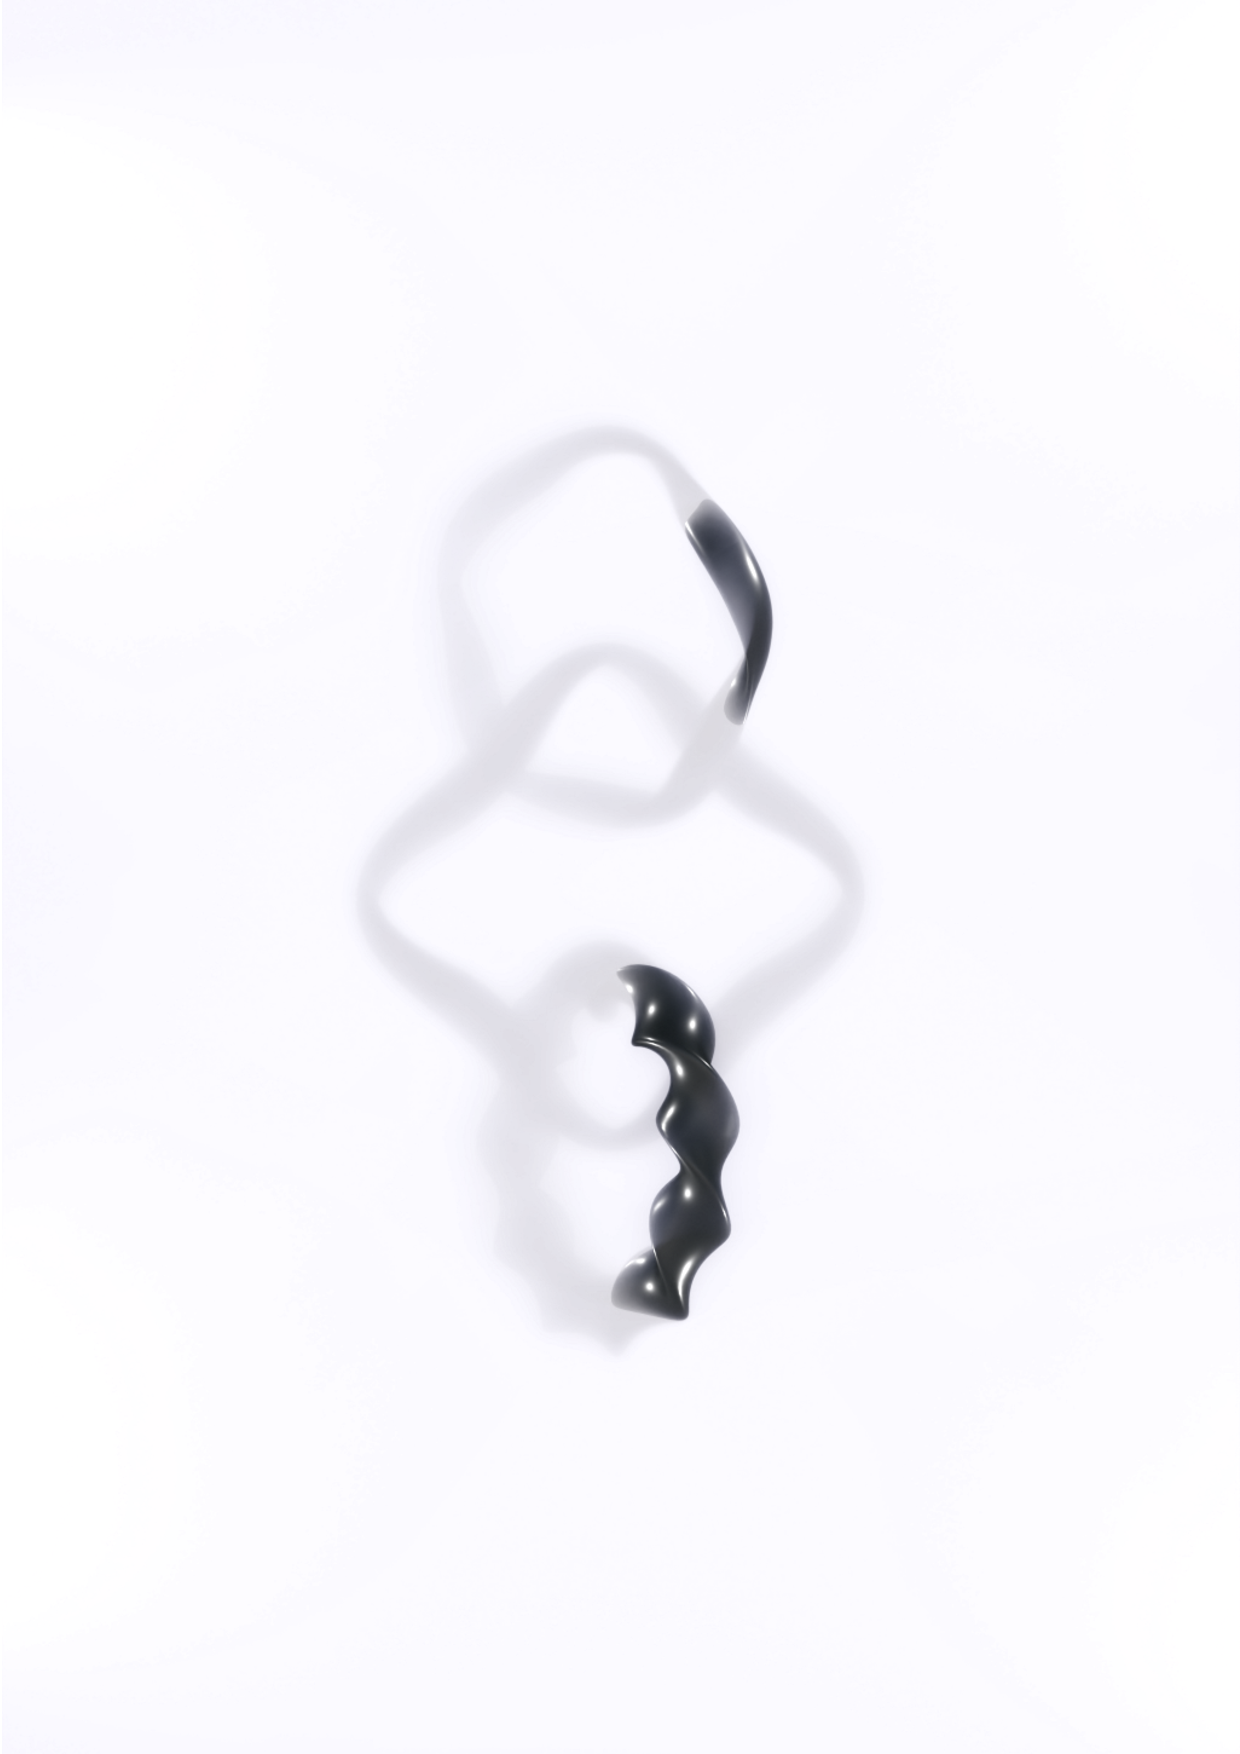
\includepdf[pages=-]{img/thesis_back.pdf}
\fi



\end{document}
%%%% THAT's ALL FOLKS **********************************************************
